\iftrue
  \documentclass[mathserif, aspectratio=1610]{intbeamer}
\else
  \documentclass[aspectratio=1610]{beamer}
  \definecolor{urllinkcol}{RGB}{31,119,180}
  \hypersetup{colorlinks,linkcolor=,urlcolor=urllinkcol}
  \usetheme{Madrid}
  \usecolortheme{dove}  % dove, whale
  \usefonttheme{professionalfonts}
  \setbeamertemplate{page number in head/foot}[appendixframenumber] % appendix pagenumbering restart
\fi

\usepackage{fourier}
\usepackage[utf8]{inputenc}
\usepackage[english]{babel}
\usepackage{subcaption}
\captionsetup[subfigure]{skip=2pt} % global setting for subfigure
\usepackage{amsmath,amssymb,amsfonts}
\usepackage{bm}
\usepackage{nicefrac}
\usepackage{trfsigns}
%\usepackage{gensymb}
%\usepackage{macros}
\usepackage{xcolor}
%\usepackage{enumerate}
\setbeamercovered{invisible}
\usepackage{tikz}
\usetikzlibrary{calc}
\usetikzlibrary {arrows.meta}
\usetikzlibrary {matrix,fit}
\usepackage{comment}
\usepackage{drawmatrix}

%\includecomment{plottikz}
%\excludecomment{plottikz}
%\definecolor{pyplotC0}{RGB}{31,119,180}
\definecolor{C0}{HTML}{1f77b4}  % column space
\definecolor{C1}{HTML}{ff7f0e}  % left null space
\definecolor{C2}{HTML}{2ca02c}  % row space
\definecolor{C3}{HTML}{d62728}
\definecolor{C4}{HTML}{9467bd}  % null space
\definecolor{C5}{HTML}{8c564b}
\definecolor{C6}{HTML}{e377c2}
\definecolor{C7}{HTML}{7f7f7f}
\definecolor{C8}{HTML}{bcbd22}
\definecolor{C9}{HTML}{17becf}

\usepackage{pgfplots}
\pgfplotsset{compat=newest}

%\newcommand{\tw}{0.73}

% ===== titlepage info =====
\title[DDASP \#24512 - Tutorial]%
{Selected Topics in Audio Signal Processing\\(Data-Driven Methods in Signal Processing) \#24512}

\author[Schultz, Spors]{%
    \underline{\href{https://orcid.org/0000-0002-3010-0294}{Frank Schultz}}, \href{https://orcid.org/0000-0001-7225-9992}{Sascha Spors}}

\date[Winter Term 2023/24]{%\raisebox{0mm}{\includegraphics[width=4.6cm]{logo.png}}\\
  Exercise -- Winter Term 2023/24}

\institute[]{Research Group Signal Processing and Virtual Acoustics\\
Institute of Communications Engineering\\
Faculty of Computer Science and Electrical Engineering\\
University of Rostock, Rostock, Germany}

\begin{document}
\maketitle
%
%
%
\input{orga}
%
%
%

\begin{frame}{Topics Proposal for Tutorial}
\begin{itemize}
\item singular value decomposition (SVD)
  \begin{itemize}
  \item 4 subspaces of a matrix
  \item left inverse, (right inverse)
  \item projection matrices
  \item dimensionality reduction of a feature space via PCA
  \end{itemize}
\item loss functions, empirical risk functions and numerical minimization, quality measures
\begin{itemize}
\item mean squared error for prediction
\item for binary, multinomial classification
\item gradient descent to find (a suitable) minimum
\item F-score, Rsquared, Goodness-Of-Fit Test
\end{itemize}
\item prediction models based on regression
    \begin{itemize}
    \item ordinary least squares (OLS)
    \item ridge regression
    \item SVD regression
    \end{itemize}
\item classifying models based on neural networks (NN)
  \begin{itemize}
  \item using fully connected layers (DNN)
  \item using convolutional layers (CNN)
  \end{itemize}
\end{itemize}
\end{frame}
% sketch of fields that contribute to data processing / data science
%
%
%
\begin{frame}{Literature}
  check textbooks in our main library
  \begin{itemize}
    \item \href{https://find.ub.uni-rostock.de/sk830}{SK830...SK840 statistics, (generalized) linear models, regression}
    \item ST 285...ST 306 machine learning, artifical intelligence, neural networks
    \item QH 212...QH 236 statistics mainly for economy, (generalized) linear models, regression
  \end{itemize}
  textbooks that I like very much
  \begin{itemize}
    \item Kevin P. Murphy (2022): "Probabilistic Machine Learning: An Introduction", MIT Press, 1st. ed.
    \href{https://probml.github.io/pml-book/book1.html}{current draft as free pdf}
    \item \href{https://math.mit.edu/~gs/}{Gilbert Strang} (2019): "Linear Algebra and Learning from Data", Wellesley, 1st ed.
  \end{itemize}
\end{frame}

\begin{frame}{Literature}
  theory textbooks that inspire me a lot
  \begin{itemize}
    \item S. Theodoridis, Machine Learning, 2nd ed. Academic Press, 2020.
    \href{https://www.sciencedirect.com/book/9780128188033/machine-learning}{free ebook}
    \item T. Hastie, R. Tibshirani, and J. Friedman, The Elements of Statistical Learning, 2nd ed. Springer, 2009.
    \href{https://hastie.su.domains/ElemStatLearn/}{free ebook}
    \item G. James, D. Witten, T. Hastie, and R. Tibshirani, An Introduction to Statistical Learning with Applications in R, 2nd ed. Springer, 2021. \href{https://www.statlearning.com/}{free ebook}
    \item I. Goodfellow, Y. Bengio, and A. Courville, Deep Learning. MIT Press, 2016.
    \item C.C. Aggarwal, Neural Networks and Deep Learning. Springer, 2018.
    \item C.C. Aggarwal, Linear Algebra and Optimization for Machine Learning. Springer, 2020. \href{https://link.springer.com/book/10.1007/978-3-030-40344-7}{free ebook}
    \item Marc P. Deisenroth, A. Aldo Faisal, Cheng S. Ong, Mathematics for Machine Learning, Cambridge, 2020. \href{https://mml-book.github.io/book/mml-book.pdf}{free ebook}
    \item Steven L. Brunton, J. Nathan Kutz, Data Driven Science \& Engineering, Cambridge, 2019. \href{http://www.databookuw.com/databook.pdf}{free ebook draft}
  \end{itemize}
\end{frame}

\begin{frame}{Resources}
  highly recommended web resources
  \begin{itemize}
    \item MIT course 18065 \href{https://ocw.mit.edu/courses/18-065-matrix-methods-in-data-analysis-signal-processing-and-machine-learning-spring-2018/}{Matrix Methods in Data Analysis, Signal Processing, and Machine Learning} by Gilbert Strang
    \item Steven L. Brunton, J. Nathan Kutz, Data Driven Science \& Engineering, Cambridge, 2019.
    \href{http://www.databookuw.com/databook.pdf}{free ebook draft},
    \href{http://www.databookuw.com/}{video lectures},
    \href{https://github.com/dylewsky/Data_Driven_Science_Python_Demos}{Python tutorials}
    \item A. G\'{e}ron, Hands-On Machine Learning with SciKit \& TensorFlow, 1st/2nd ed. O'Reilly, 2017/2019.
    \href{https://github.com/ageron/handson-ml2}{Python tutorials}
    \item \href{https://playground.tensorflow.org}{A Neural Network Playground---TensorFlow}
    \item courses by Andrew Ng at \url{https://www.deeplearning.ai/} and/or \url{https://www.coursera.org/}
  \end{itemize}
\end{frame}

\begin{frame}{Textbooks on Statistics}
    ML deals with stuff that is actually known for decades (at least the linear modeling part), so if we are really
    serious about to learn it deeply, we should think over concepts on
    statistical signal processing, maximum-likelihood, Bayesian vs. frequentist
    statistics, generalized linear models, hierarchical models ... ...

    textbooks that I like very much
  \begin{itemize}
  \item L. Fahrmeir, A. Hamerle, and G. Tutz, Multivariate statistische Verfahren, 2nd ed. de Gruyter, 1996.
  \href{https://www.degruyter.com/document/doi/10.1515/9783110816020/html}{free ebook}
  \item L. Fahrmeir, T. Kneib, S. Lang, and B. D. Marx, Regression, 2nd ed. Springer, 2021.
  \item A. J. Dobson and A. G. Barnett, An Introduction to Generalized Linear Models, 4th ed. CRC Press, 2018.
  \item H. Madsen, P. Thyregod, Introduction to General and Generalized Linear Models, CRC Press, 2011.
  \item A. Agresti, Foundations of Linear and Generalized Models, Wiley, 2015.
  \end{itemize}
\end{frame}




\begin{comment}
\section{Ex01: Introduction}
\begin{frame}{Ex01: Introduction}
Objectives
\begin{itemize}
\item related fields for data science / learning from data
\item model concept, un- \& supervised learning, prediction
\item idea of model parameters and hyper parameters
\item structured workflow for proper data learning
\item audio toy example that is used for linear regression and SVD demo
\end{itemize}
\end{frame}

\begin{frame}{Structured Development of Data-Driven Methods}
\textbf{Established Procedure}
\begin{enumerate}
\item Definition of the problem and of performance measures
\item Data preparation and feature extraction
\item Spot check potential model architectures
\item Model selection
\item Evaluation and reporting
\item Application
\end{enumerate}
\textbf{Technical Aspects}
\begin{itemize}
\item identify independent / dependent variables, prepare them
\item check for potential error measures and quality measures
\item choose model type(s), identify potential model parameters and hyper parameters
\item proper data handling with train/validate/test data sets
\item train/fit model(s) including optimized hyper parameters
\item choose best model(s), final train, final test, report quality
\end{itemize}
% sketch and explain x->model->y on blackboard
\end{frame}


\begin{frame}{We Can Do Machine Learning with a Linear Model}
linear algebra\footnote{we should do ourselves a favour and read at least one of the linear algebra textbooks by Gilbert Strang}
is THE tool to handle linear models
\begin{center}
$
\def\Mic{3}
\def\LS{1}
\drawmatrix[fill=none, height=\Mic, width=0]y_\mathtt{M \times 1} =
\drawmatrix[fill=none, height=\Mic, width=\LS]X_\mathtt{M \times N}
\drawmatrix[fill=none, height=\LS, width=0]\theta_\mathtt{M \times 1} +
\drawmatrix[fill=none, height=\Mic, width=0]n_\mathtt{M \times 1}
$
\end{center}
\vspace{5mm}
\begin{equation*}
\bm{y} = \bm{X} \,\,\, \bm{\theta} + \bm{n}
\end{equation*}

$\bm{y}$ output data

$\bm{X}$ features as columns in a feature matrix

$\bm{\theta}$ model parameters (which we want to learn)

$\bm{n}$ noise (included in the measured output data)

\end{frame}


\begin{frame}{Audio Toy Example for Linear Regression and SVD}
Consider the following linear combinations
$$\bm{X} \bm{\theta} + \bm{n} = \bm{y}$$
where $\bm{\theta}=[\theta_0, \theta_1, \theta_2, ..., \theta_{N-1}]^\mathrm{T}$ are typical variables for the model parameter vector.
%
\begin{itemize}
\item $\bm{X}_{M \times N}$ matrix with $M$ audio samples for each column, $n$-th column represents the $n$-th audiotrack
\item $\bm{\theta}_{N \times 1}$ column vector of scalar values that represent a dedicated gain for each audiotrack
\item $\bm{n}_{M \times 1}$ column vector that represents an $M$-sample long noise signal added to the mixdown $\bm{X} \bm{\theta}$
\item $\bm{y}_{M \times 1}$ audio signal with $M$ samples as a result of the linear combination plus noise
\end{itemize}
%
Let us assume that i) we know $\bm{X}$ (i.e. the individual audio tracks) and $\bm{y}$ (i.e. the noise-corrupted final mixdown), ii) that we do not know the noise $\bm{n}$ and iii) that we want to estimate the 'real world' mixing gains $\bm{\theta}$
% sketch Xb=y
\end{frame}


\section{Section I: SVD / 4 Subspaces / Pseudo-Inverse}

\begin{frame}{Ex02 / Ex03: SVD and 4 Subspaces of a Matrix}
Objectives
\begin{itemize}
\item recap important matrix factorizations
\item recap eigenvalues/eigenvectors
\item spectral theorem
\item SVD and 4 subspaces within orthonormal bases $\bm{V}$, $\bm{U}$
\item rank-1 matrix superposition
\end{itemize}
\end{frame}



\begin{frame}{Matrix Factorization from Eigenwert Problem for Square Matrix}

for square matrix $\bm{A}_{M \times M}$ we can have a factorization (known as diagonalization)

$$\bm{A} = \bm{X} \bm{\Lambda} \bm{X}^{-1}$$

(but only) when $M$ independent eigenvectors as columns in $\bm{X}$ (only then $\bm{X}^{-1}$ is possible)

with the corresponding eigenvalues $\lambda$ in the diagonal matrix $\Lambda$

\begin{center}
$
\def\M{1}
\def\N{1}
\def\rank{0.9999}
\drawmatrix[fill=none, height=\M, width=\N]A_\mathtt{M \times M} =
\drawmatrix[bbox style={fill=C4}, bbox height=\M, bbox width=\M, fill=C0, height=\M, width=\rank\N]X_\mathtt{M \times M}
\drawmatrix[diag]\Lambda_\mathtt{M \times M}
\drawmatrix[bbox style={fill=C4}, bbox height=\N, bbox width=\N, fill=C0, height=\N, width=\rank\N]{X}_\mathtt{M \times M}^{-1}
$
\end{center}

the matrix is acting onto $m$-th eigenvector as

$$\bm{A} \bm{x}_m = \lambda_m \bm{x}_m$$

$\Lambda$ might be complex-valued

$\bm{X}$ might be complex-valued

if $\lambda_m=0$ we get $\bm{A} \bm{x}_m = 0 \cdot \bm{x}_m = \bm{0}$, i.e. $\bm{A}$ is a singular matrix, i.e. $\bm{A}$ is a non-full rank matrix

rank of matrix $\bm{A}$ is $R$ == number of non-zero eigenvalues

\end{frame}




\begin{frame}{Matrix Factorization from Eigenwert Problem for Symmetric Matrix}

for \underline{symmetric} matrix $\bm{A}_{M \times M} = \bm{A}_{M \times M}^H$ we can have a special case of diagonalization

$$\bm{A} = \bm{Q} \bm{\Lambda} \bm{Q}^{-1} = \bm{Q} \bm{\Lambda} \bm{Q}^{H}$$

(only) when $M$ independent, \underline{orthogonal} eigenvectors as columns in $\bm{Q}$ \quad($\bm{Q} \bm{Q}^H = \bm{I}$, $\bm{Q}^H \bm{Q} = \bm{I}$)

with the corresponding eigenvalues $\lambda\in\mathbb{R}$ in the diagonal matrix $\Lambda$

\begin{center}
$
\def\M{1}
\def\N{1}
\def\rank{0.9999}
\drawmatrix[fill=none, height=\M, width=\N]A_\mathtt{M \times M} =
\drawmatrix[bbox style={fill=C4}, bbox height=\M, bbox width=\M, fill=C1, height=\M, width=\rank\N]{Q}_\mathtt{M \times M}
\drawmatrix[diag]\Lambda_\mathtt{M \times M}
\drawmatrix[bbox style={fill=C4}, bbox height=\N, bbox width=\N, fill=C1, height=\N, width=\rank\N]{Q}_\mathtt{M \times M}^{H}
$
\end{center}

the matrix is acting onto the $m$-th eigenvector as

$$\bm{A} \bm{q}_m = \lambda_m \bm{q}_m$$

$\bm{\Lambda}\in\mathbb{R}$

$\bm{Q}\in\mathbb{R}$ if $\bm{A}\in\mathbb{R}$, $\bm{Q}\in\mathbb{C}$ if $\bm{A}\in\mathbb{C}$

if $\lambda_m=0$ we get $\bm{A} \bm{q}_m = 0 \cdot \bm{q}_m = \bm{0}$, i.e. $\bm{A}$ is a singular matrix, i.e. $\bm{A}$ is a non-full rank matrix

rank of matrix $\bm{A}$ is $R$ == number of non-zero eigenvalues
\end{frame}





\begin{frame}[t]{Matrix Factorization from Eigenwert Problem for Symmetric Matrix}

for a normal matrix $\bm{A}$ (such as symmetric, i.e. $\bm{A}^H \bm{A} = \bm{A} \bm{A}^H$ )

there is the fundamental spectral theorem
$$\bm{A} = \bm{Q} \bm{\Lambda} \bm{Q}^{H}$$

i.e. diagonalization in terms of eigenvectors in full rank matrix $\bm{Q}$ and eigenvalues in $\bm{\Lambda}\in\mathbb{R}$

What does $\bm{A}$ with an eigenvector $\bm{q}$?

\begin{flushleft}
$
\def\M{1}
\def\N{1}
\def\rank{0.9999}
\drawmatrix[fill=none, height=\M, width=\N]A_\mathtt{M \times M}
\drawmatrix[fill=none, height=\M, width=0]q_\mathtt{M \times 1}
=
\drawmatrix[bbox style={fill=C4}, bbox height=\M, bbox width=\M, fill=C1, height=\M, width=\rank\N]{Q}_\mathtt{M \times M}
\drawmatrix[diag]\Lambda_\mathtt{M \times M}
\drawmatrix[bbox style={fill=C4}, bbox height=\N, bbox width=\N, fill=C1, height=\N, width=\rank\N]{Q}_\mathtt{M \times M}^{H}
\drawmatrix[fill=none, height=\M, width=0]q_\mathtt{M \times 1} = ?
$

%$$\bm{A} \bm{q} = \bm{Q} \bm{\Lambda} \bm{Q}^{H} \bm{q} = ?$$
\end{flushleft}

\end{frame}







\begin{frame}{Generalized Factorization?!}
Over-Determined (tall/thin matrix $\bm{A}$)
\begin{center}
$
\def\M{3}
\def\N{1}
\def\rank{0.8}
\drawmatrix[fill=none, height=\M, width=\N]A_\mathtt{M \times N} =
\drawmatrix[bbox style={fill=C4}, bbox height=\M, bbox width=\M, fill=C0, height=\M, width=\rank\N]U_\mathtt{M \times M}
\drawmatrix[bbox style={fill=gray!50}, bbox height=\M, bbox width=\N, fill=white, height=\rank\N, width=\rank\N]\Sigma_\mathtt{M \times N}
\drawmatrix[bbox style={fill=C1}, bbox height=\N, bbox width=\N, fill=C2, height=\N, width=\rank\N]{V}_\mathtt{N \times N}^H
$
\end{center}
Under-Determined (flat/fat aka short/wide matrix $\bm{A}$)
\begin{center}
$
\def\M{1}
\def\N{3}
\def\rank{0.2}
\drawmatrix[fill=none, height=\M, width=\N]A_\mathtt{M \times N} =
\drawmatrix[bbox style={fill=C4}, bbox height=\M, bbox width=\M, fill=C0, height=\M, width=\rank\M]U_\mathtt{M \times M}
\drawmatrix[bbox style={fill=gray!50}, bbox height=\M, bbox width=\N, fill=white, height=\rank\M, width=\rank\M]\Sigma_\mathtt{M \times N}
\drawmatrix[bbox style={fill=C1}, bbox height=\N, bbox width=\N, fill=C2, height=\N, width=\rank\M]{V}_\mathtt{N \times N}^H
$
\end{center}
\end{frame}



\begin{frame}{Generalized Factorization: Singular Value Decomposition (SVD)}
most general matrix factorization for a matrix $\bm{A}$ with rank $R$

fundamentally important for understanding the heart beat of linear algebra

\begin{center}
$
\def\M{2}
\def\N{1}
\def\rank{0.999999}
\drawmatrix[fill=none, height=\M, width=\N]A_\mathtt{M \times N} =
\drawmatrix[bbox style={fill=C4}, bbox height=\M, bbox width=\M, fill=C0, height=\M, width=\rank\N]U_\mathtt{M \times M}
\drawmatrix[bbox style={fill=gray!50}, bbox height=\M, bbox width=\N, fill=white, height=\rank\N, width=\rank\N]\Sigma_\mathtt{M \times N}
\drawmatrix[bbox style={fill=C1}, bbox height=\N, bbox width=\N, fill=C2, height=\N, width=\rank\N]{V}_\mathtt{N \times N}^H
$
\end{center}

\begin{center}
$
\def\M{1}
\def\N{2}
\def\rank{0.999999}
\drawmatrix[fill=none, height=\M, width=\N]A_\mathtt{M \times N} =
\drawmatrix[bbox style={fill=C4}, bbox height=\M, bbox width=\M, fill=C0, height=\M, width=\rank\M]U_\mathtt{M \times M}
\drawmatrix[bbox style={fill=gray!50}, bbox height=\M, bbox width=\N, fill=white, height=\rank\M, width=\rank\M]\Sigma_\mathtt{M \times N}
\drawmatrix[bbox style={fill=C1}, bbox height=\N, bbox width=\N, fill=C2, height=\N, width=\rank\M]{V}_\mathtt{N \times N}^H
$
\end{center}

$$\bm{A} = \bm{U} \bm{\Sigma} \bm{V}^\mathrm{H}\qquad \qquad \bm{U}\bm{U}^H = \bm{U}^H\bm{U} = \bm{I}_{M \times M} \qquad \qquad \bm{V}\bm{V}^H = \bm{V}^H\bm{V} = \bm{I}_{N \times N}$$


left singular vectors\quad$\bm{U} = \mathrm{eigvec}(\bm{A}\bm{A}^\mathrm{H})$
\begin{footnotesize}, order must match to the corresponding singular values\end{footnotesize}

right singular vectors $\bm{V} = \mathrm{eigvec}(\bm{A}^\mathrm{H}\bm{A})$
\begin{footnotesize}, order must match to the corresponding singular values\end{footnotesize}

singular value matrix $\bm{\Sigma}$
\begin{footnotesize}, $\text{min}(M,N)$ singular values on \underline{diagonal} descending order, $R$ of them non-zero
\end{footnotesize}


\end{frame}





\begin{frame}[label=SVD1]{Singular Value Decomposition (SVD)}

\begin{flushleft}
$
\def\M{1.4}
\def\N{1}
\def\rank{0.4}
\drawmatrix[fill=none, height=\M, width=\N]A_\mathtt{M \times N} =
\drawmatrix[bbox style={fill=C4}, bbox height=\M, bbox width=\M, fill=C0, height=\M, width=\rank\N]U_\mathtt{M \times M}
\drawmatrix[bbox style={fill=gray!50}, bbox height=\M, bbox width=\N, fill=white, height=\rank\N, width=\rank\N]\Sigma_\mathtt{M \times N}
\drawmatrix[bbox style={fill=C1}, bbox height=\N, bbox width=\N, fill=C2, height=\N, width=\rank\N]{V}_\mathtt{N \times N}^H
$
\end{flushleft}

\begin{flushleft}
$
\def\M{1}
\def\N{1.4}
\def\rank{0.7}
\drawmatrix[fill=none, height=\M, width=\N]A_\mathtt{M \times N} =
\drawmatrix[bbox style={fill=C4}, bbox height=\M, bbox width=\M, fill=C0, height=\M, width=\rank\M]U_\mathtt{M \times M}
\drawmatrix[bbox style={fill=gray!50}, bbox height=\M, bbox width=\N, fill=white, height=\rank\M, width=\rank\M]\Sigma_\mathtt{M \times N}
\drawmatrix[bbox style={fill=C1}, bbox height=\N, bbox width=\N, fill=C2, height=\N, width=\rank\M]{V}_\mathtt{N \times N}^H
$
\end{flushleft}

%$$\bm{A} = \bm{U} \bm{\Sigma} \bm{V}^\mathrm{H}$$

\vspace{3.25cm}

left singular vectors\quad$\bm{U} = \mathrm{eigvec}(\bm{A}\bm{A}^\mathrm{H})$
\begin{footnotesize}, order must match to the corresponding singular values\end{footnotesize}

right singular vectors $\bm{V} = \mathrm{eigvec}(\bm{A}^\mathrm{H}\bm{A})$
\begin{footnotesize}, order must match to the corresponding singular values\end{footnotesize}

singular value matrix $\bm{\Sigma}$
\begin{footnotesize}, $\text{min}(M,N)$ singular values on \underline{diagonal} descending order, $R$ of them non-zero
\end{footnotesize}

\end{frame}














\begin{frame}{Singular Value Decomposition (SVD)}

\begin{flushleft}
$
\def\M{1.4}
\def\N{1}
\def\rank{0.4}
\drawmatrix[fill=none, height=\M, width=\N]A_\mathtt{M \times N} =
\drawmatrix[bbox style={fill=C4}, bbox height=\M, bbox width=\M, fill=C0, height=\M, width=\rank\N]U_\mathtt{M \times M}
\drawmatrix[bbox style={fill=gray!50}, bbox height=\M, bbox width=\N, fill=white, height=\rank\N, width=\rank\N]\Sigma_\mathtt{M \times N}
\drawmatrix[bbox style={fill=C1}, bbox height=\N, bbox width=\N, fill=C2, height=\N, width=\rank\N]{V}_\mathtt{N \times N}^H
$
\end{flushleft}

\begin{flushleft}
$
\def\M{1}
\def\N{1.4}
\def\rank{0.7}
\drawmatrix[fill=none, height=\M, width=\N]A_\mathtt{M \times N} =
\drawmatrix[bbox style={fill=C4}, bbox height=\M, bbox width=\M, fill=C0, height=\M, width=\rank\M]U_\mathtt{M \times M}
\drawmatrix[bbox style={fill=gray!50}, bbox height=\M, bbox width=\N, fill=white, height=\rank\M, width=\rank\M]\Sigma_\mathtt{M \times N}
\drawmatrix[bbox style={fill=C1}, bbox height=\N, bbox width=\N, fill=C2, height=\N, width=\rank\M]{V}_\mathtt{N \times N}^H
$
\end{flushleft}

$$\bm{A}
\begin{bmatrix}
\bm{v}_1 & \bm{v}_2 & \bm{v}_R & \bm{v}_N
\end{bmatrix}
= $$

$$\bm{A}
\begin{bmatrix}
\bm{v}_1 & \bm{v}_2 & \bm{v}_R & \bm{v}_N
\end{bmatrix}
= $$

\vspace{1.5cm}

left singular vectors\quad$\bm{U} = \mathrm{eigvec}(\bm{A}\bm{A}^\mathrm{H})$
\begin{footnotesize}, order must match to the corresponding singular values\end{footnotesize}

right singular vectors $\bm{V} = \mathrm{eigvec}(\bm{A}^\mathrm{H}\bm{A})$
\begin{footnotesize}, order must match to the corresponding singular values\end{footnotesize}

singular value matrix $\bm{\Sigma}$
\begin{footnotesize}, $\text{min}(M,N)$ singular values on \underline{diagonal} descending order, $R$ of them non-zero
\end{footnotesize}
\end{frame}





\begin{frame}{Singular Value Decomposition (SVD)}

\begin{flushleft}
$
\def\M{1.4}
\def\N{1}
\def\rank{0.4}
\drawmatrix[fill=none, height=\M, width=\N]A_\mathtt{M \times N} =
\drawmatrix[bbox style={fill=C4}, bbox height=\M, bbox width=\M, fill=C0, height=\M, width=\rank\N]U_\mathtt{M \times M}
\drawmatrix[bbox style={fill=gray!50}, bbox height=\M, bbox width=\N, fill=white, height=\rank\N, width=\rank\N]\Sigma_\mathtt{M \times N}
\drawmatrix[bbox style={fill=C1}, bbox height=\N, bbox width=\N, fill=C2, height=\N, width=\rank\N]{V}_\mathtt{N \times N}^H
$
\end{flushleft}

\begin{flushleft}
$
\def\M{1}
\def\N{1.4}
\def\rank{0.7}
\drawmatrix[fill=none, height=\M, width=\N]A_\mathtt{M \times N} =
\drawmatrix[bbox style={fill=C4}, bbox height=\M, bbox width=\M, fill=C0, height=\M, width=\rank\M]U_\mathtt{M \times M}
\drawmatrix[bbox style={fill=gray!50}, bbox height=\M, bbox width=\N, fill=white, height=\rank\M, width=\rank\M]\Sigma_\mathtt{M \times N}
\drawmatrix[bbox style={fill=C1}, bbox height=\N, bbox width=\N, fill=C2, height=\N, width=\rank\M]{V}_\mathtt{N \times N}^H
$
\end{flushleft}

\vspace{0.75cm}

$$\bm{A}
\begin{bmatrix}
a \textcolor{C2}{\bm{v}_1} & b \textcolor{C2}{\bm{v}_2} & c \textcolor{C2}{\bm{v}_R} & \dots & y \textcolor{C1}{\bm{v}_{N-1}} & z \textcolor{C1}{\bm{v}_N}
\end{bmatrix}
=
\begin{bmatrix}
a \sigma_1 \textcolor{C0}{\bm{u}_1} & b \sigma_2 \textcolor{C0}{\bm{u}_2} & c \sigma_R \textcolor{C0}{\bm{u}_R} & \dots & \bm{0} & \bm{0}
\end{bmatrix}
\rightarrow
\bm{A} \bm{V} = \bm{\Sigma} \bm{U}
$$
$$\bm{A}
\begin{bmatrix}
a \textcolor{C2}{\bm{v}_1} + b \textcolor{C2}{\bm{v}_2} + c \textcolor{C2}{\bm{v}_R} + \dots + y \textcolor{C1}{\bm{v}_{N-1}} + z \textcolor{C1}{\bm{v}_N}
\end{bmatrix}
=
[a \sigma_1 \textcolor{C0}{\bm{u}_1} + b \sigma_2 \textcolor{C0}{\bm{u}_2} + c \sigma_R \textcolor{C0}{\bm{u}_R} + \dots + \bm{0} + \bm{0}]
$$

\vspace{0.75cm}

left singular vectors\quad$\bm{U} = \mathrm{eigvec}(\bm{A}\bm{A}^\mathrm{H})$
\begin{footnotesize}, order must match to the corresponding singular values\end{footnotesize}

right singular vectors $\bm{V} = \mathrm{eigvec}(\bm{A}^\mathrm{H}\bm{A})$
\begin{footnotesize}, order must match to the corresponding singular values\end{footnotesize}

singular value matrix $\bm{\Sigma}$
\begin{footnotesize}, $\text{min}(M,N)$ singular values on \underline{diagonal} descending order, $R$ of them non-zero
\end{footnotesize}
\end{frame}

%\againframe{SVD1}





\begin{frame}{The 4 Subspaces of a Matrix}

matrix $\bm{A}_{M \times N}$ spans four fundamental subspaces

\hspace{4.25cm}
\textcolor{C0}{column space} $\perp$ \textcolor{C4}{left null space}
\hspace{0.75cm}
\textcolor{C2}{row space} $\perp$ \textcolor{C1}{null space}

\textcolor{C0}{column space / range / image in U:} $$\text{Range}(\bm{A}) = \{\bm{b}\in\mathbb{C}^M | \bm{A} \bm{x} = \bm{b},\qquad\forall \bm{x}\in\mathbb{C}^N\}$$

\textcolor{C1}{null space / kernel in V:} $$\text{Null}(\bm{A}) = \{\bm{x}\in\mathbb{C}^N | \bm{A} \bm{x} = \bm{0}\}$$

the column/null-space concept for transposed matrix $\bm{A}^H$ yields the two other spaces:

\textcolor{C2}{row space in V:} $$\text{Range}(\bm{A}^H) = \{\bm{x}\in\mathbb{C}^N | \bm{A}^H \bm{b} = \bm{x},\qquad\forall \bm{b}\in\mathbb{C}^M\}$$

\textcolor{C4}{left null space / cokernel in U:} $$\text{Null}(\bm{A}^H) = \{\bm{b}\in\mathbb{C}^M | \bm{A}^H \bm{b} = \bm{0}\}$$

matrix rank of $\bm{A}$ is $R\leq \text{min}(M,N)$ == dimension of column space == dimension of row space == number of independent columns and rows
== number of pivots in rref($\bm{A}$)

\end{frame}



\begin{frame}[t]{SVD and the 4 Subspaces of a Matrix}
%
\begin{flushleft}
$
\def\M{2}
\def\N{1}
\def\rank{0.15}
\drawmatrix[fill=none, height=\M, width=\N]A_\mathtt{M \times N} =
\drawmatrix[bbox style={fill=C4}, bbox height=\M, bbox width=\M, fill=C0, height=\M, width=\rank\N]U_\mathtt{M \times M}
\drawmatrix[bbox style={fill=gray!50}, bbox height=\M, bbox width=\N, fill=white, height=\rank\N, width=\rank\N]\Sigma_\mathtt{M \times N}
\drawmatrix[bbox style={fill=C1}, bbox height=\N, bbox width=\N, fill=C2, height=\N, width=\rank\N]{V}_\mathtt{N \times N}^H
$
\end{flushleft}

What is the rank of $\bm{A}_1$?

What is
the \textcolor{C0}{column space},
the \textcolor{C4}{null space},
the \textcolor{C2}{row space} and
the \textcolor{C1}{left null space}
of $\bm{A}_1$?


\begin{center}
$
\def\M{2}
\def\N{1}
\def\rank{0.9999}
\drawmatrix[fill=none, height=\M, width=\N]{A_1}_\mathtt{M \times N}
=
\sigma_1 \cdot
\drawmatrix[fill=none, height=\M, width=0]{u_1}_\mathtt{M \times 1}
\drawmatrix[fill=none, height=0, width=\N]{v_1^H}_\mathtt{1 \times N} \approx
\drawmatrix[fill=none, height=\M, width=\N]{A}_\mathtt{M \times N}
$
\end{center}


\end{frame}








\begin{frame}[t]{Simple Numerical Example for the 4 Subspaces}

matrix factorization in terms of column space $\times$ row space
$$
\bm{C} =
\begin{bmatrix}
1 & 0 \\ 0 & 2 \\ 0 & 0
\end{bmatrix}
\qquad
\bm{R} =
\begin{bmatrix}
3 & 0 \\ 0 & 4
\end{bmatrix}
\qquad
\bm{A} =
\bm{C} \bm{R} =
\begin{bmatrix}
3 & 0 \\ 0 & 8 \\ 0 & 0
\end{bmatrix}
$$
matrix factorization in terms of SVD
$$
\bm{A} = \bm{U} \bm{\Sigma} \bm{V}^H
=
\begin{bmatrix}
0 & 1 & 0 \\
1 & 0 & 0 \\
0 & 0 & 1
\end{bmatrix}
%
\begin{bmatrix}
8 & 0\\
0 & 3\\
0 & 0
\end{bmatrix}
%
\left(
\begin{bmatrix}
0 & 1\\
1 & 0
\end{bmatrix}
\right)^H
$$

What is the rank of $\bm{A}$?

What are the four subspaces of $\bm{A}$? Give them as equations and as a sketch...

\end{frame}




\begin{frame}{SVD Fundamentals}
%
superposition of rank-1 matrices (outer products) because singular values in diagonal matrix $\bm{\Sigma}$
$$\bm{A}_{M \times N} = \sum_{r=1}^{\text{rank }R} \sigma_r \bm{u}_r \bm{v}_r^\mathrm{H} = \bm{U} \bm{S} \bm{V}^\mathrm{H}$$
%
input-related matrix $\bm{V}$ and output related matrix $\bm{U}$ are unitary, i.e.
$$\bm{V}\bm{V}^\mathrm{H}=\bm{I},\quad\bm{V}^\mathrm{H}\bm{V}=\bm{I},\quad\bm{U}\bm{U}^\mathrm{H}=\bm{I},\quad\bm{U}^\mathrm{H}\bm{U}=\bm{I}$$
%
due to $\bm{V}^\mathrm{H}\bm{V}=\bm{I}$ we can re-arrange
$$\bm{A} = \bm{U} \bm{\Sigma} \bm{V}^\mathrm{H} \rightarrow
\bm{A} \bm{V} = \bm{U} \bm{\Sigma}$$
rank $R$ matrix $\bm{A}$ acting on \textcolor{C2}{row space} $\bm{v}$ maps to corresponding \textcolor{C0}{column space / range / image} $\bm{u}$ weighted by corresponding singular value $\sigma$
$$\bm{A} \textcolor{C2}{\bm{v}_{1...R}} = \sigma_{1...R} \textcolor{C0}{\bm{u}_{1...R}}$$
rank $R$ matrix $\bm{A}$ matrix acting on \textcolor{C1}{null space / kernel} $\bm{v}$ maps to zero vector $\bm{0}_{M \times 1}$
$$\bm{A} \textcolor{C1}{\bm{v}_{R+1...N}} = \bm{0}$$


\end{frame}


\begin{frame}[t]{SVD Example Manual Calculus: Problem Definition and First Expectations}
We should calculate the SVD of the simple $M \times N$ matrix
$$\bm{X} =
\begin{bmatrix}
1\\2
\end{bmatrix}
\begin{bmatrix}
1 & 3
\end{bmatrix}
=
\begin{bmatrix}
1 & 3\\
2 & 6
\end{bmatrix}
\stackrel{?}{=}
\bm{U}\bm{S}\bm{V}^\mathrm{T}
$$
manually.

Before, we start, let us realize what we have here.

The single outer product tells us immediately that we deal with a rank $r=1$ matrix, expecting dependencies
in rows and columns.

We immediately see that i) rows are dependent because row2 = 2 row1, ii) columns are dependent because col2 = 3 col1.

Due to rank $R=1$, we expect only one non-zero singular value $\sigma_1$, therefore the dimension
of row space (which is always equal to the dimension of column space) is $R=1$, i.e. we have $R$
independent vectors that span the row space and $r$ independent vectors that span the column space, so these spaces are lines in both 2D spaces in our example.

The $\bm{U}$ space has vectors in $\mathbb{R}^{M=2}$, the $\bm{V}$ space has vectors in $\mathbb{R}^{N=2}$.

\end{frame}


\begin{frame}[t]{SVD Example Manual Calculus: Further Expectations I}
$$\bm{X} =
\begin{bmatrix}
1\\2
\end{bmatrix}
\begin{bmatrix}
1 & 3
\end{bmatrix}
=
\begin{bmatrix}
1 & 3\\
2 & 6
\end{bmatrix}
$$

This simple single outer product gives us direct access to the column space, as this is a $\bm{X}=\bm{C}\bm{R}$ factorization; it is the line along the column vector
$$
\begin{bmatrix}
1\\2
\end{bmatrix}
$$
Furthermore, we directly can deduce the row space, which is the line along the
column vector
$$
\begin{bmatrix}
1\\3
\end{bmatrix},
$$
i.e. the transposed row found in the outer product. So, all $\bm{X}^\mathrm{T} \bm{y}$,
except those solutions that produce $\bm{X}^\mathrm{T} \bm{y} = \bm{0}$ (these $\bm{y}$
belong to the left null space), are multiples of $[1, 3]^\mathrm{T}$.


\end{frame}



\begin{frame}[t]{SVD Example Manual Calculus: Further Expectations II}
$$\bm{X} =
\begin{bmatrix}
1\\2
\end{bmatrix}
\begin{bmatrix}
1 & 3
\end{bmatrix}
=
\begin{bmatrix}
1 & 3\\
2 & 6
\end{bmatrix}
\stackrel{?}{=}
\bm{U}\bm{S}\bm{V}^\mathrm{T}
$$

As we have $M-R$ vectors that span the left null space, thus here $M=2$ and $R=1$,
the left nullspace is a line orthogonal to the column space (which is also a line).

As we have $N-R$ vectors that span the null space, thus here $N=2$ and $R=1$,
the nullspace is a line orthogonal to the row space (which is also a line).

We deal with $\mathbb{R}^{M=2}$ and $\mathbb{R}^{N=2}$ dimensions, so each space
is 2D, so no more than two independent lines are possible in these spaces.

We should meet these expectations, when calculating the SVD manually.

\end{frame}




\begin{frame}[t]{SVD Example Manual Calculus: Eigenvalue And -Vector Problem}
$$\bm{X} =
\begin{bmatrix}
1 & 3\\
2 & 6
\end{bmatrix}
\stackrel{?}{=}
\bm{U}\bm{S}\bm{V}^\mathrm{T}
$$

Let us start with
$\bm{X}^\mathrm{T} \bm{X} = (\bm{U}\bm{S}\bm{V}^\mathrm{T})^\mathrm{T} (\bm{U}\bm{S}\bm{V}^\mathrm{T})
= \bm{V}\bm{S}^\mathrm{T}\bm{U}^\mathrm{T} \bm{U}\bm{S}\bm{V}^\mathrm{T}
= \bm{V}\bm{S}^\mathrm{T}\bm{S}\bm{V}^\mathrm{T}
$
using the property of SVD matrices $\bm{U}^\mathrm{T} \bm{U} = \bm{I}$

$$\bm{X}^\mathrm{T} \bm{X} =
\begin{bmatrix}
1 & 2\\
3 & 6
\end{bmatrix}
\begin{bmatrix}
1 & 3\\
2 & 6
\end{bmatrix}
$$
1st column of $\bm{X}^\mathrm{T} \bm{X}$
comes from the linear combination
$\begin{bmatrix}
1 & 2\\
3 & 6
\end{bmatrix}
\begin{bmatrix}
1 \\ 2
\end{bmatrix}
=
1
\begin{bmatrix}
1\\
3
\end{bmatrix}
+2
\begin{bmatrix}
2\\
6
\end{bmatrix}
=
\begin{bmatrix}
5\\
15
\end{bmatrix}
$

2nd column of $\bm{X}^\mathrm{T} \bm{X}$
comes from the linear combination
$\begin{bmatrix}
1 & 2\\
3 & 6
\end{bmatrix}
\begin{bmatrix}
3 \\ 6
\end{bmatrix}
=
3
\begin{bmatrix}
1\\
3
\end{bmatrix}
+6
\begin{bmatrix}
2\\
6
\end{bmatrix}
=
\begin{bmatrix}
15\\
45
\end{bmatrix}
$

$$\bm{X}^\mathrm{T} \bm{X} = \begin{bmatrix}
5 & 15\\
15 & 45
\end{bmatrix}$$
has dependent rows and columns, hence, rank 1

\end{frame}


\begin{frame}[t]{SVD Example Manual Calculus: Eigenvalue And -Vector Problem}
$$\bm{X}^\mathrm{T} \bm{X} =
\bm{V}\bm{S}^\mathrm{T}\bm{S}\bm{V}^\mathrm{T} =
\begin{bmatrix}
5 & 15\\
15 & 45
\end{bmatrix}$$
The matrix factorization in the middle stores eigenvectors in $\bm{V}$ and
corresponding eigenvalues in $\bm{S}^\mathrm{T}\bm{S}$ of the matrix
$\bm{X}^\mathrm{T} \bm{X}$.
We need to calculate them, so we take the usual steps
$$\mathrm{det}(\bm{X}^\mathrm{T} \bm{X} - \lambda \bm{I}) = 0$$

$$\bm{X}^\mathrm{T} \bm{X} - \lambda \bm{I} =
\begin{bmatrix}
5-\lambda & 15\\
15 & 45-\lambda
\end{bmatrix}$$

$$\mathrm{det}(\begin{bmatrix}
5-\lambda & 15\\
15 & 45-\lambda
\end{bmatrix}) =
(5-\lambda)(45-\lambda) - 15^2 = \lambda^2-50\lambda = 0$$

$$\lambda_1 = 50\quad \lambda_2 = 0$$

\end{frame}



\begin{frame}[t]{SVD Example Manual Calculus: Eigenvalue And -Vector Problem}
For
$$\lambda_1 = 50\quad \lambda_2 = 0$$
we shall find the corresponding eigenvectors
$$\bm{X}^\mathrm{T} \bm{X} \bm{v}_1 = \lambda_1 \bm{v}_1\quad
\bm{X}^\mathrm{T} \bm{X} \bm{v}_1 = \lambda_2 \bm{v}_1$$
Rearranging
$$
(\bm{X}^\mathrm{T} \bm{X} - \lambda_1 \bm{I} )\bm{v_1} = \bm{0}\quad
(\bm{X}^\mathrm{T} \bm{X} - \lambda_2 \bm{I} )\bm{v_2} = \bm{0}
$$
Inserting numbers (we should see that $\bm{v}_1$ and $\bm{v}_2$ are nullspace vectors for these two matrices)
$$
\begin{bmatrix}
5-50 & 15\\
15 & 45-50
\end{bmatrix}
\bm{v}_1
=
\begin{bmatrix}
0 \\0
\end{bmatrix}\quad
\begin{bmatrix}
5-0 & 15\\
15 & 45-0
\end{bmatrix}
\bm{v}_2
=
\begin{bmatrix}
0 \\0
\end{bmatrix}
$$
Solving the set of linear equations yields
$$
\begin{bmatrix}
-45 & 15\\
15 & -5
\end{bmatrix}
\begin{bmatrix}
1 \\3
\end{bmatrix}
=
\begin{bmatrix}
0 \\0
\end{bmatrix}\quad
\begin{bmatrix}
5 & 15\\
15 & 45
\end{bmatrix}
\begin{bmatrix}
3 \\-1
\end{bmatrix}
=
\begin{bmatrix}
0 \\0
\end{bmatrix}
$$
\end{frame}

\begin{frame}[t]{SVD Example Manual Calculus: Singular Value And Right Singular Vectors}

Let us normalize all eigenvectors to unit length vectors
$
\bm{v}_1 =
\frac{1}{\sqrt{10}}
\begin{bmatrix}
1 \\3
\end{bmatrix}$ and
$
\bm{v}_2 =
\frac{1}{\sqrt{10}}
\begin{bmatrix}
3 \\-1
\end{bmatrix}
$

We got only one non-zero eigenvalue $\lambda_{r=1} = 50$ and the corresponding
eigenvector
$$\bm{v}_{r=1} =
\frac{1}{\sqrt{10}}
\begin{bmatrix}
1 \\3
\end{bmatrix}$$

We sort the $r=1...R$ eigenvalues (and keep it linked to their
corresponding eigenvectors) in decreasing order, i.e. $\lambda_1 > \lambda_2 >... >\lambda_R \neq 0$.

The sorted! eigenvectors of $\bm{X}^\mathrm{T} \bm{X}$ are the sorted (unit length)
right singular vectors $\bm{v}_i$ of $\bm{X}$, these span the row space. In our example
the spanned row space is $\bm{v}_{1}$, i.e. a line in 2D.

The sorted! (non-zero) eigenvalues $\lambda_r$ become the sorted! singular values $\sigma_r = \sqrt{\lambda_r}$, these are used by the matrix to map row space stuff to column space and vice versa.

Now, we use the SVD property
$\bm{X} \bm{v}_{r=1...R} = \sigma_{r=1...R} \bm{u}_{r=1...R}$
to find the corresponding $r$-th unit vector $\bm{u}_r$ in the column space, simply by
$\bm{X} \bm{v}_{r} \frac{1}{\sigma_r} = \bm{u}_{r}$ (this is the textbook approach, real algorithms don't do this, numerical linear algebra is tough science!)

\end{frame}

\begin{frame}[t]{SVD Example Manual Calculus: Towards Left Singular Vectors}

So, with $\sigma_1 = \sqrt{\lambda_1} = \sqrt{50}$ and $\bm{v}_{r=1=R} =
\frac{1}{\sqrt{10}}
\begin{bmatrix}
1 \\3
\end{bmatrix}$
we can find $\bm{X} \bm{v}_{1} \frac{1}{\sigma_1} = \bm{u}_{1}$ as
$$\bm{u}_{1} = \begin{bmatrix}
1 & 3\\
2 & 6
\end{bmatrix}
\frac{1}{\sqrt{10}}
\begin{bmatrix}
1 \\3
\end{bmatrix}
\frac{1}{\sqrt{50}}
=
\frac{1}{\sqrt{500}}
(1
\begin{bmatrix}
1\\
2
\end{bmatrix}
+
3
\begin{bmatrix}
3\\
6
\end{bmatrix})
=
\frac{1}{\sqrt{500}}
\begin{bmatrix}
10\\
20
\end{bmatrix},
$$
which is already a unit length vector. As we only have one non-zero singular value, $\bm{u}_{1}$ completely spans the column space, which is a line in 2D space.

What we got so far? We might want to check that $\bm{X} \bm{v}_1 = \sigma_1 \bm{u}_1$ holds with the found solutions

$$
\sigma_1 = \sqrt{50}\qquad
\bm{v}_1=
\frac{1}{\sqrt{10}}
\begin{bmatrix}
1 \\3
\end{bmatrix}\qquad
\bm{u}_1 =
\frac{1}{\sqrt{5}}
\begin{bmatrix}
1\\
2
\end{bmatrix}
$$
As we have only one non-zero singular value, the full rank matrix approximation (just this one outer product from the general SVD equation $\bm{X} = \sum_{r=1}^{R} \sigma_r  \bm{u}_r \bm{v}^\mathrm{T}_r$)
$$\sigma_1  \bm{u}_1 \bm{v}^\mathrm{T}_1
= \sqrt{50} \frac{1}{\sqrt{5}}
\begin{bmatrix}
1\\
2
\end{bmatrix}
\frac{1}{\sqrt{10}}
\begin{bmatrix}
1 & 3
\end{bmatrix}
=
\begin{bmatrix}
1\\
2
\end{bmatrix}
\begin{bmatrix}
1 & 3
\end{bmatrix}
=
\begin{bmatrix}
1 & 3\\
2 & 6
\end{bmatrix}=\bm{X}
$$
already yields exactly $\bm{X}$ where we started from. We, however need to finish the SVD...
\end{frame}



\begin{frame}[t]{SVD Example Manual Calculus: Nullspace}
The null space is spanned by all these vectors from our above eigenwert problem,
which belong to a zero eigenvalue. By definition they are all orthogonal.
We calculated one unit length vector for the null space
$
\bm{v}_2 =
\frac{1}{\sqrt{10}}
\begin{bmatrix}
3 \\-1
\end{bmatrix},
$
hence, the null space is spanned by a line in 2D space.
We could re-check that the null space definition $\bm{X} \bm{v}_2 = \bm{0}$ holds:
$$
\begin{bmatrix}
1 & 3\\
2 & 6
\end{bmatrix}
\frac{1}{\sqrt{10}}
\begin{bmatrix}
3 \\-1
\end{bmatrix}
=\frac{1}{\sqrt{10}}
(3\begin{bmatrix}
1 \\
2
\end{bmatrix}
-1
\begin{bmatrix}
 3\\
 6
\end{bmatrix})=\bm{0}
$$

We know from the solved eigenwert problem, that $\bm{v_1} \perp \bm{v_2}$, it's easy to re-check this.

Here in this example, this confirms that row space spanned by $\bm{v_1}$ is orthogonal to null space spanned by $\bm{v_2}$ .

So, the full right singular value matrix and singular value matrix  are set up as

$$
\bm{V} =
\begin{bmatrix}
\bm{v_1} & \bm{v_2}
\end{bmatrix}
=\frac{1}{\sqrt{10}}
\begin{bmatrix}
1 & 3 \\
3 & -1
\end{bmatrix}
\qquad
\bm{S}=
\begin{bmatrix}
\lambda_1 \neq 0 & 0\\
0 & 0
\end{bmatrix}
=
\begin{bmatrix}
\sqrt{50} & 0\\
0 & 0
\end{bmatrix}
$$
\end{frame}

\begin{frame}[t]{SVD Example Manual Calculus: Left Nullspace}
We obviously cannot follow $\bm{X} \bm{v} = \sigma \bm{u}$ to find missing
$\bm{u}_2$, because there is no corresponding $\sigma$ that acts as meaningful mapping.

Instead, we could solve the dedicated eigenwert problem
$$\bm{X} \bm{X}^\mathrm{T} \bm{u}_1 = \lambda_1 \bm{u}_1\quad
\bm{X} \bm{X}^\mathrm{T} \bm{u}_2 = \lambda_2 \bm{u}_2$$
to find out that again $\lambda_1 = 50$, $\lambda_2=0$.

Furthermore, the already known $\bm{u}_1$ is spaning the column space, as this has the singular value $\sigma_1 = \sqrt{\lambda_1}$, which is linked to $\bm{v}_1$ spanning the row space.

$\bm{u}_2$ corresponds to $\lambda_2=0$, so certainly no column space stuff, it then must be left null space.

In this simple matrix example, we can derive $\bm{u}_2$ very easy with the left null space definition (as we have only to find this one vector)

$$\bm{X}^\mathrm{T} \bm{u_2} = \bm{0}$$

$$
\begin{bmatrix}
1 & 2\\
3 & 6
\end{bmatrix}
\bm{u_2}
=
\begin{bmatrix}0\\0\end{bmatrix}
\rightarrow
\begin{bmatrix}
1 & 2\\
3 & 6
\end{bmatrix}
\begin{bmatrix}2\\-1\end{bmatrix}
=
2
\begin{bmatrix}
1\\
3
\end{bmatrix}
-1
\begin{bmatrix}
2\\
6
\end{bmatrix}
=
\begin{bmatrix}0\\0\end{bmatrix}
\rightarrow
\bm{u}_2 = \begin{bmatrix}2\\-1\end{bmatrix}
$$


\end{frame}

\begin{frame}[t]{SVD Example Manual Calculus: Final Result}
We make this a unit length vector as required for the SVD
$$
\bm{u}_2 = \frac{1}{\sqrt{5}}\begin{bmatrix}2\\-1\end{bmatrix}
$$
We might re-check that $\bm{u}_1 \perp \bm{u}_2$, which again tells us
that column space spanned by $\bm{u}_1$ is orthogonal to left null space spanned by $\bm{u}_2$

So, the full left singular value matrix is set up as


$$
\bm{U} =
\begin{bmatrix}
\bm{u}_1 & \bm{u}_2
\end{bmatrix}=
\frac{1}{\sqrt{5}}
\begin{bmatrix}
1 & 2\\
2 & -1
\end{bmatrix}
$$

So, if there are no typos (statistics tells us there should be ;-))
we end up in
$$
\bm{X}
=
\begin{bmatrix}
1 & 3\\
2 & 6
\end{bmatrix}
= \bm{U} \bm{S} \bm{V}^\mathrm{T}=
\begin{bmatrix}
\frac{1}{\sqrt{5}} & \frac{2}{\sqrt{5}}\\
\frac{2}{\sqrt{5}} & \frac{-1}{\sqrt{5}}
\end{bmatrix}
\cdot
\begin{bmatrix}
\sqrt{50} & 0\\
0 & 0
\end{bmatrix}
\cdot
\left(
\begin{bmatrix}
\frac{1}{\sqrt{10}} & \frac{3}{\sqrt{10}} \\
\frac{3}{\sqrt{10}} & \frac{-1}{\sqrt{10}}
\end{bmatrix}
\right)^\mathrm{T}
$$
which in Python and Matlab produces unattractive numbers in the SVD data due to the square root involved.
So we should better know what we are doing and what to expect from the SVD.
\end{frame}














\begin{frame}{4 Subspaces of a Matrix}
%
every matrix $\bm{A}_{M \times N} = \bm{U} \bm{\Sigma} \bm{V}^H$ spans four fundamental subspaces

$\bm{U}$ and $\bm{V}$ span the 4 subspaces of matrix $\bm{A}$ in the (probably) most elegant way

\hspace{0.75cm}
in $\bm{V}$: \textcolor{C2}{row space} $\perp$ \textcolor{C1}{null space}
\hspace{2cm}
in $\bm{U}$: \textcolor{C0}{column space} $\perp$ \textcolor{C4}{left null space}

\centering
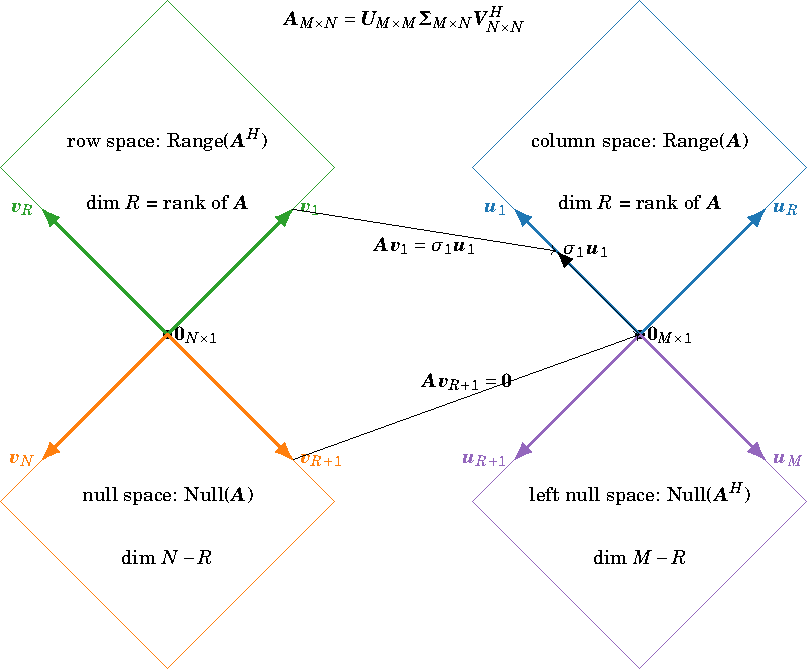
\includegraphics[width=0.5\textwidth]{four_subspaces.pdf}

\hspace{0.75cm}
right singular vectors in $\bm{V}$
\hspace{4.5cm}
left singular vectors in $\bm{U}$

\end{frame}






\begin{frame}[label=SubspacesForSketch, t]{4 Subspaces of a Matrix - Examples for Special Matrix Characteristics}

\hspace{-0.5cm}
\textcolor{C2}{row space} $\perp$ \textcolor{C1}{null space}
\hspace{0.5cm}
\textcolor{C0}{column space} $\perp$ \textcolor{C4}{left null space}

\begin{flushleft}
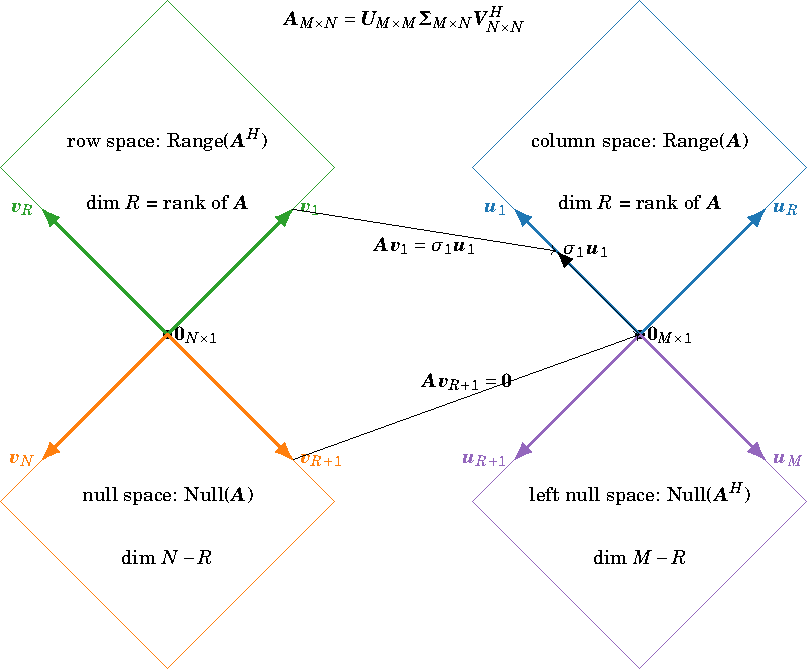
\includegraphics[width=0.5\textwidth]{four_subspaces.pdf}
\end{flushleft}

\hspace{-0.5cm}
right singular vectors in $\bm{V}$
\hspace{0.5cm}
left singular vectors in $\bm{U}$

\end{frame}

\againframe{SubspacesForSketch}
\againframe{SubspacesForSketch}
\againframe{SubspacesForSketch}

\begin{frame}{Singular Value Decomposition (SVD), full rank cases}

$\cdot$ Sum of rank-1 matrices\qquad
$\bm{A} = \bm{U} \bm{\Sigma} \bm{V}^H =  \sum\limits_{r=1}^{R} \sigma_r \quad \textcolor{C0}{\bm{u}}_r \quad \textcolor{C2}{\bm{v}}^H_r$

\hspace{4.25cm}
\textcolor{C0}{column space} $\perp$ \textcolor{C4}{left null space}
\hspace{0.75cm}
\textcolor{C2}{row space} $\perp$ \textcolor{C1}{null space}

$\cdot$ Square matrix $\bm{A}$, \quad $M$ rows $=$ $N$ columns, \quad full rank ($r=M=N$), \quad inverse $\bm{A}^\dagger = \bm{A}^{-1}$
\begin{center}
$
\def\M{1}
\def\N{1}
\def\rank{0.999999}
\drawmatrix[fill=none, height=\M, width=\N]A_\mathtt{M \times N} =
\drawmatrix[bbox style={fill=C4}, bbox height=\M, bbox width=\M, fill=C0, height=\M, width=\rank\N]U_\mathtt{M \times M}
\drawmatrix[bbox style={fill=gray!50}, bbox height=\M, bbox width=\N, fill=white, height=\rank\N, width=\rank\N]\Sigma_\mathtt{M \times N}
\drawmatrix[bbox style={fill=C1}, bbox height=\N, bbox width=\N, fill=C2, height=\N, width=\rank\N]{V}_\mathtt{N \times N}^H
$
\end{center}
$\cdot$ Flat / fat matrix $\bm{A}$, \quad $M$ rows $<$ $N$ columns, \quad full row rank ($r=M$), \quad right inverse $\bm{A}^{\dagger_r} = \bm{A}^H (\bm{A} \bm{A}^H )^{-1}$
such that $\bm{A} \bm{A}^{\dagger_r} = \bm{I}$ (i.e. projection to row space)
\begin{center}
$
\def\M{1}
\def\N{1.4}
\def\rank{0.999999}
\drawmatrix[fill=none, height=\M, width=\N]A_\mathtt{M \times N} =
\drawmatrix[bbox style={fill=C4}, bbox height=\M, bbox width=\M, fill=C0, height=\M, width=\rank\M]U_\mathtt{M \times M}
\drawmatrix[bbox style={fill=gray!50}, bbox height=\M, bbox width=\N, fill=white, height=\rank\M, width=\rank\M]\Sigma_\mathtt{M \times N}
\drawmatrix[bbox style={fill=C1}, bbox height=\N, bbox width=\N, fill=C2, height=\N, width=\rank\M]{V}_\mathtt{N \times N}^H
$
\end{center}
$\cdot$ Tall / thin matrix $\bm{A}$, \quad $M$ rows $>$ $N$ columns, \quad full column rank ($r=N$), \quad left inverse $\bm{A}^{\dagger_l} = (\bm{A}^H \bm{A})^{-1} \bm{A}^H$ such that $\bm{A}^{\dagger_l} \bm{A} = \bm{I}$ (i.e. projection to row space)
\begin{center}
$
\def\M{1.4}
\def\N{1}
\def\rank{0.999999}
\drawmatrix[fill=none, height=\M, width=\N]A_\mathtt{M \times N} =
\drawmatrix[bbox style={fill=C4}, bbox height=\M, bbox width=\M, fill=C0, height=\M, width=\rank\N]U_\mathtt{M \times M}
\drawmatrix[bbox style={fill=gray!50}, bbox height=\M, bbox width=\N, fill=white, height=\rank\N, width=\rank\N]\Sigma_\mathtt{M \times N}
\drawmatrix[bbox style={fill=C1}, bbox height=\N, bbox width=\N, fill=C2, height=\N, width=\rank\N]{V}_\mathtt{N \times N}^H
$
\end{center}
\end{frame}
%
%
%
\begin{frame}{Singular Value Decomposition (SVD), not full-rank cases}

$\cdot$ Sum of rank-1 matrices\qquad
$\bm{A} = \bm{U} \bm{\Sigma} \bm{V}^H =  \sum\limits_{r=1}^{R} \sigma_r \quad \textcolor{C0}{\bm{u}}_r \quad \textcolor{C2}{\bm{v}}^H_r$

$\cdot$ not full-rank cases need (general) pseudo-inverse $\bm{A}^\dagger = \bm{V} \Sigma^\dagger \bm{U}^H$

\hspace{4.25cm}
\textcolor{C0}{column space} $\perp$ \textcolor{C4}{left null space}
\hspace{0.75cm}
\textcolor{C2}{row space} $\perp$ \textcolor{C1}{null space}

$\cdot$ Square matrix $\bm{A}$, \quad $M$ rows $=$ $N$ columns, \quad not full-rank ($r<M=N$)
\begin{center}
$
\def\M{1}
\def\N{1}
\def\rank{0.5}
\drawmatrix[fill=none, height=\M, width=\N]A_\mathtt{M \times N} =
\drawmatrix[bbox style={fill=C4}, bbox height=\M, bbox width=\M, fill=C0, height=\M, width=\rank\N]U_\mathtt{M \times M}
\drawmatrix[bbox style={fill=gray!50}, bbox height=\M, bbox width=\N, fill=white, height=\rank\N, width=\rank\N]\Sigma_\mathtt{M \times N}
\drawmatrix[bbox style={fill=C1}, bbox height=\N, bbox width=\N, fill=C2, height=\N, width=\rank\N]{V}_\mathtt{N \times N}^H
$
\end{center}
$\cdot$ Flat / fat matrix $\bm{A}$, \quad $M$ rows $<$ $N$ columns, \quad not full-rank ($r<M$)
\begin{center}
$
\def\M{1}
\def\N{1.4}
\def\rank{0.75}
\drawmatrix[fill=none, height=\M, width=\N]A_\mathtt{M \times N} =
\drawmatrix[bbox style={fill=C4}, bbox height=\M, bbox width=\M, fill=C0, height=\M, width=\rank\M]U_\mathtt{M \times M}
\drawmatrix[bbox style={fill=gray!50}, bbox height=\M, bbox width=\N, fill=white, height=\rank\M, width=\rank\M]\Sigma_\mathtt{M \times N}
\drawmatrix[bbox style={fill=C1}, bbox height=\N, bbox width=\N, fill=C2, height=\N, width=\rank\M]{V}_\mathtt{N \times N}^H
$
\end{center}
$\cdot$ Tall / thin matrix $\bm{A}$, \quad $M$ rows $>$ $N$ columns, \quad not full-rank ($r<N$)
\begin{center}
$
\def\M{1.4}
\def\N{1}
\def\rank{0.67}
\drawmatrix[fill=none, height=\M, width=\N]A_\mathtt{M \times N} =
\drawmatrix[bbox style={fill=C4}, bbox height=\M, bbox width=\M, fill=C0, height=\M, width=\rank\N]U_\mathtt{M \times M}
\drawmatrix[bbox style={fill=gray!50}, bbox height=\M, bbox width=\N, fill=white, height=\rank\N, width=\rank\N]\Sigma_\mathtt{M \times N}
\drawmatrix[bbox style={fill=C1}, bbox height=\N, bbox width=\N, fill=C2, height=\N, width=\rank\N]{V}_\mathtt{N \times N}^H
$
\end{center}
\end{frame}

% \begin{frame}{Subspace Properties and Characteristics of Inverse Problem}
% %
% sketches of the 4 subspaces for these 4 cases help to get the essence how a matrix maps things forward and (potentially) backward
% %
% \begin{itemize}
% \item full rank, no nullspace, no left null space = square matrix = exactly solvable, typically learned in basic linear algebra course
% \item full column rank, no nullspace, potentially large left nullspace = tall/thin matrix, over determined system of equations, we need the left inverse, many practical problems, statistical model fitting, least squares error solution
% \item full row rank, potentially large nullspace, no left nullspace = flat/fat matrix, under-determined system of equations, we need the right inverse, solution in the sense of least squares magnitude for unknown vector
% \item rank deficient, potentially large nullspace, potentially large left nullspace, meaningful information of the matrix is not stored in optimum way $\rightarrow$ data-driven learning...but before doing this stuff, we should at least learn full column rank cases properly
% \end{itemize}
% %
% \end{frame}


\begin{frame}[t]{Ex04: Recap 4 Subspaces of a Matrix}

\hspace{-0.5cm}
\textcolor{C2}{row space} $\perp$ \textcolor{C1}{null space}
\hspace{0.5cm}
\textcolor{C0}{column space} $\perp$ \textcolor{C4}{left null space}
\hspace{0.5cm}
Projection:

\begin{flushleft}
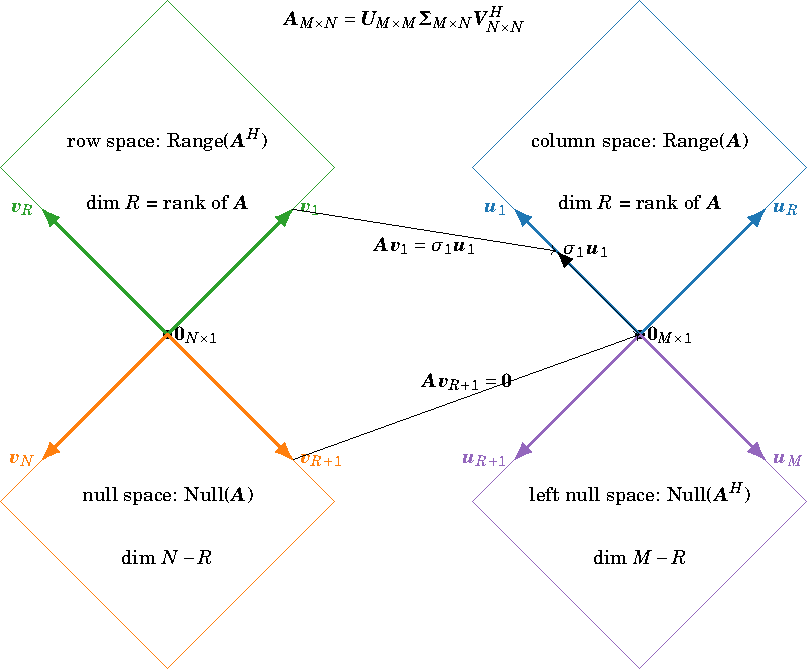
\includegraphics[width=0.5\textwidth]{four_subspaces.pdf}
\end{flushleft}

\hspace{-0.5cm}
right singular vectors in $\bm{V}$
\hspace{0.5cm}
left singular vectors in $\bm{U}$

\end{frame}




\begin{frame}[t]{Ex04: Solving an Inverse Problem == Finding Model Parameters}
feature matrix $\bm{X}$ as full column rank with rank $R=2$ (2 independent columns = 2 independent rows = 2 non-zero singular values)
$$
\bm{X} =
\begin{bmatrix}
3 & 0 \\ 0 & 8 \\ 0 & 0
\end{bmatrix}
=
\begin{bmatrix}
0 & 1 & 0 \\
1 & 0 & 0 \\
0 & 0 & 1
\end{bmatrix}
%
\begin{bmatrix}
8 & 0\\
0 & 3\\
0 & 0
\end{bmatrix}
%
\left(
\begin{bmatrix}
0 & 1\\
1 & 0
\end{bmatrix}
\right)^H=
\bm{U} \bm{\Sigma} \bm{V}^H
$$

Can we solve for the model parameter vector $\bm{\theta}$ given the feature matrix $\bm{X}$ and the output data vector $\bm{y}$?
%
If no, why? If yes, how?
$$
\bm{X} \bm{\theta} = \bm{y}
\quad \rightarrow \quad
\begin{bmatrix}
3 & 0 \\ 0 & 8 \\ 0 & 0
\end{bmatrix}
\begin{bmatrix}
\bm{\theta} \\ |
\end{bmatrix}=
\begin{bmatrix}
-3 \\ 4 \\ 2
\end{bmatrix}
$$

\end{frame}



\begin{frame}[t]{Finding Model Parameters with Calculus}
%
$$
\begin{bmatrix}
3 & 0 \\ 0 & 8 \\ 0 & 0
\end{bmatrix}
\begin{bmatrix}
\hat{\bm{\theta}} \\ |
\end{bmatrix}=
\begin{bmatrix}
-3 \\ 4 \\ 2
\end{bmatrix}
$$
%
optimization problem in least squares sense: $\min_{\text{wrt }\bm{\theta}} \lVert\bm{e}\rVert_2^2 = \min_{\text{wrt }\bm{\theta}} \lVert\bm{y} - \bm{X} \bm{\theta}\rVert_2^2$
%

recall that $\lVert\bm{y} - \bm{X} \bm{\theta}\rVert_2^2 = (\bm{y} - \bm{X} \bm{\theta})^H (\bm{y} - \bm{X} \bm{\theta})$
\begin{align*}
\lVert \bm{y} - \bm{X} \bm{\theta}\rVert_2  &= \sqrt{(-3 - 3\theta_1)^2 + (4-8\theta_2)^2 + (0-2)^2}\\
J(\theta_1, \theta_2) = \lVert\bm{y} - \bm{X} \bm{\theta}\rVert_2^2 &= (-3 - 3\theta_1)^2 + (4-8\theta_2)^2 + (0-2)^2
\end{align*}
%
$$
\nabla J(\theta_1, \theta_2) =
\begin{bmatrix}
\frac{\partial J}{\partial \theta_1}\\
\frac{\partial J}{\partial \theta_2}
\end{bmatrix}
=
\begin{bmatrix}
2 (-3) (-3 - 3\theta_1)
\\
2 (-8) (4-8\theta_2)
\end{bmatrix}
=
\begin{bmatrix}
18 (1 + \theta_1)
\\
128 (-\frac{1}{2}+\theta_2)
\end{bmatrix}
$$
%
minimum at $\nabla J(\theta_1, \theta_2) = \bm{0}$, hence
%
$$
\hat{\bm{\theta}}
=
\begin{bmatrix}
\hat{\theta_1}
\\
\hat{\theta_2}
\end{bmatrix}
=
\begin{bmatrix}
-1
\\
\frac{1}{2}
\end{bmatrix}
$$


\end{frame}














\begin{frame}[t]{Finding Model Parameters with Subspace Fundamentals}

Can we solve for the model parameter vector $\bm{\theta}$ given the feature matrix $\bm{X}$ and the output data vector $\bm{y}$?
%
If no, why? If yes, how?
$$
\begin{bmatrix}
3 & 0 \\ 0 & 8 \\ 0 & 0
\end{bmatrix}
\begin{bmatrix}
\bm{\theta} \\ |
\end{bmatrix}=
\begin{bmatrix}
-3 \\ 4 \\ 2
\end{bmatrix}
%
\qquad\qquad
\bm{X} =
\begin{bmatrix}
3 & 0 \\ 0 & 8 \\ 0 & 0
\end{bmatrix}
=
\begin{bmatrix}
0 & 1 & 0 \\
1 & 0 & 0 \\
0 & 0 & 1
\end{bmatrix}
%
\begin{bmatrix}
8 & 0\\
0 & 3\\
0 & 0
\end{bmatrix}
%
\left(
\begin{bmatrix}
0 & 1\\
1 & 0
\end{bmatrix}
\right)^H=
\bm{U} \bm{\Sigma} \bm{V}^H
$$

\begin{center}
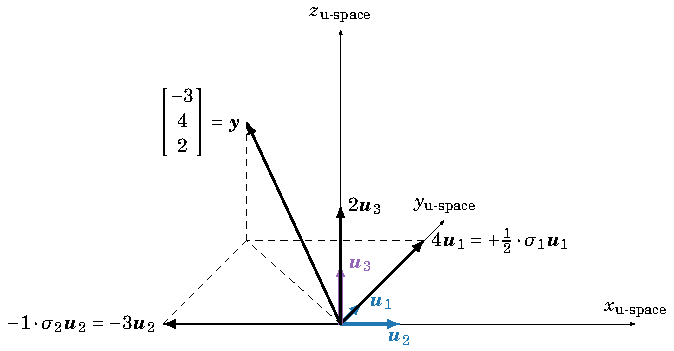
\includegraphics[width=0.7\textwidth]{least_squares_error.pdf}
\end{center}


\end{frame}







\begin{frame}[t]{Finding Model Parameters with Subspace Fundamentals / Left Inverse}
%
\begin{center}
\textcolor{C0}{column space} $\perp$ \textcolor{C4}{left null space}\\
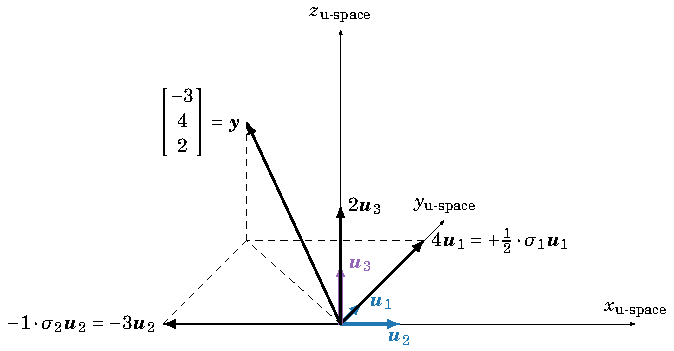
\includegraphics[width=0.5\textwidth]{least_squares_error.pdf}
\end{center}
%
$$\bm{X} \hat{\bm{\theta}} + \bm{e} = \bm{y} \qquad \rightarrow \qquad \bm{e} = \bm{y} - \bm{X} \hat{\bm{\theta}}$$
%
shortest path of $\bm{e}$ to column space means that $\bm{e}$ is orthogonal to column space

hence, $\bm{e}$ must live purely in left null space, i.e. $\bm{X}^H \bm{e} = \bm{0}$ holds, this yields
%
$$\bm{X}^H (\bm{y} - \bm{X} \hat{\bm{\theta}}) = \bm{0} \quad \rightarrow \quad \bm{X}^H \bm{y} = \bm{X}^H \bm{X} \hat{\bm{\theta}} \quad \rightarrow \quad
(\bm{X}^H \bm{X})^{-1} \bm{X}^H \bm{y} = \hat{\bm{\theta}}
$$

middle equation: normal equations, right equation: least squares error solution using left inverse $\bm{X}^{\dagger_l} = (\bm{X}^H \bm{X})^{-1} \bm{X}^H$ such that
$\bm{X}^{\dagger_l} \bm{X} = \bm{I}$


\end{frame}


\begin{frame}{Left Inverse via SVD Mindset}
we want to solve for ${\bm{\theta}}$, full column rank $\bm{X}_{M \times N}$, rank $R=N$
$$\bm{X} {\bm{\theta}} = \bm{y}$$
apply SVD:
$$\bm{U} \bm{\Sigma} \bm{V}^\mathrm{H} {\bm{\theta}} = \bm{y}$$
get the weights for U space projection:
$$\bm{U}^\mathrm{H} \bm{U} \bm{\Sigma} \bm{V}^\mathrm{H} {\bm{\theta}} = \bm{U}^\mathrm{H}\bm{y}$$
invert all singular values and set up $\bm{\Sigma}^{\dagger_l}_{N \times M} = [\mathrm{diag}(1/\sigma_i) \quad \bm{0}]$ such that
$\bm{\Sigma}^{\dagger_l}\bm{\Sigma} = \bm{I}_{N \times N}$

apply $\bm{\Sigma}^{\dagger_l}$ left:
$$\bm{\Sigma}^{\dagger_l}\bm{\Sigma} \bm{V}^\mathrm{H} {\bm{\theta}} = \bm{\Sigma}^{\dagger_l}\bm{U}^\mathrm{H}\bm{y}$$
let matrix $\bm{V}$ act on this vector, i.e. map as linear combination into row space in $\bm{V}$
$$\bm{V} \bm{V}^\mathrm{H} {\bm{\theta}} = \bm{V} \bm{\Sigma}^{\dagger_l}\bm{U}^\mathrm{H}\bm{y}
\rightarrow \text{this yields our estimator } \hat{\bm{\theta}} = \bm{V} \bm{\Sigma}^{\dagger_l}\bm{U}^\mathrm{H}\bm{y} = \bm{X}^{\dagger_l} \bm{y}$$
we might want to show that the left inverse $\bm{X}^{\dagger_l}$ can be written equivalently as
$$\bm{X}^{\dagger_l} = \bm{V} \bm{\Sigma}^{\dagger_l}\bm{U}^\mathrm{H} = (\bm{X}^\mathrm{H}\bm{X})^{-1} \bm{X}^\mathrm{H}$$
\end{frame}












\begin{frame}[t]{Left Inverse via another SVD Mindset I}

we meanwhile know that for left inverse characteristics $$\bm{X}^{\dagger_l} \bm{X} = \bm{I}$$

this is a projection matrix into the row space of $\bm{X}$, because $\bm{X}^{\dagger_l} \bm{X} \bm{\theta} = \bm{I} \bm{\theta}$

factor this with SVD

$$\bm{V} \,\,\bm{?}\,\, \bm{U}^H \bm{U} \bm{\Sigma} \bm{V}^H = \bm{I}$$

\begin{center}
$
\def\M{1.8}
\def\N{1}
\def\rank{0.999999}
\drawmatrix[bbox style={fill=C1}, bbox height=\N, bbox width=\N, fill=C2, height=\N, width=\rank\N]{V}_\mathtt{N \times N}
\drawmatrix[fill=none, height=\N, width=\M]?_\mathtt{N \times M}
\drawmatrix[bbox style={fill=C4}, bbox height=\M, bbox width=\M, fill=C0, height=\M, width=\rank\N]U^H_\mathtt{M \times M}
\drawmatrix[bbox style={fill=C4}, bbox height=\M, bbox width=\M, fill=C0, height=\M, width=\rank\N]U_\mathtt{M \times M}
\drawmatrix[bbox style={fill=gray!50}, bbox height=\M, bbox width=\N, fill=white, height=\rank\N, width=\rank\N]\Sigma_\mathtt{M \times N}
\drawmatrix[bbox style={fill=C1}, bbox height=\N, bbox width=\N, fill=C2, height=\N, width=\rank\N]{V}_\mathtt{N \times N}^H=
\drawmatrix[diag]I_\mathtt{N \times N}
$
\end{center}

\end{frame}





\begin{frame}[t]{Left Inverse via another SVD Mindset II}

we meanwhile know that for left inverse characteristics $$\bm{X}^{\dagger_l} \bm{X} = \bm{I}$$

this is a projection matrix into the row space of $\bm{X}$, because $\bm{X}^{\dagger_l} \bm{X} \bm{\theta} = \bm{I} \bm{\theta}$

factor this with SVD

$$\bm{V} \,\,\bm{?}\,\, \bm{\Sigma} \bm{V}^H = \bm{I}$$

\begin{center}
$
\def\M{1.8}
\def\N{1}
\def\rank{0.999999}
\drawmatrix[bbox style={fill=C1}, bbox height=\N, bbox width=\N, fill=C2, height=\N, width=\rank\N]{V}_\mathtt{N \times N}
\drawmatrix[fill=none, height=\N, width=\M]?_\mathtt{N \times M}
\drawmatrix[bbox style={fill=gray!50}, bbox height=\M, bbox width=\N, fill=white, height=\rank\N, width=\rank\N]\Sigma_\mathtt{M \times N}
\drawmatrix[bbox style={fill=C1}, bbox height=\N, bbox width=\N, fill=C2, height=\N, width=\rank\N]{V}_\mathtt{N \times N}^H=
\drawmatrix[diag]I_\mathtt{N \times N}
$
\end{center}

\end{frame}




\begin{frame}[t]{Left Inverse via another SVD Mindset III}

we meanwhile know that for left inverse characteristics $$\bm{X}^{\dagger_l} \bm{X} = \bm{I}$$

this is a projection matrix into the row space of $\bm{X}$, because $\bm{X}^{\dagger_l} \bm{X} \bm{\theta} = \bm{I} \bm{\theta}$

factor this with SVD

$$\bm{?}\,\, \bm{\Sigma} = \bm{I}$$

\begin{center}
$
\def\M{1.8}
\def\N{1}
\def\rank{0.999999}
\drawmatrix[fill=none, height=\N, width=\M]?_\mathtt{N \times M}
\drawmatrix[bbox style={fill=gray!50}, bbox height=\M, bbox width=\N, fill=white, height=\rank\N, width=\rank\N]\Sigma_\mathtt{M \times N}=
\drawmatrix[diag]I_\mathtt{N \times N}
$
\end{center}

\end{frame}




\begin{frame}[t]{Left Inverse via another SVD Mindset IV}

we meanwhile know that for left inverse characteristics $$\bm{X}^{\dagger_l} \bm{X} = \bm{I}$$

this is a projection matrix into the row space of $\bm{X}$, because $\bm{X}^{\dagger_l} \bm{X} \bm{\theta} = \bm{I} \bm{\theta}$

factor this with SVD

$$\bm{\Sigma}^{\dagger_l} \bm{\Sigma} = \bm{I}$$

\begin{center}
$
\def\M{1.8}
\def\N{1}
\def\rank{0.999999}
\drawmatrix[fill=none, height=\N, width=\M]{\Sigma^{\dagger_l}}_\mathtt{N \times M}
\drawmatrix[bbox style={fill=gray!50}, bbox height=\M, bbox width=\N, fill=white, height=\rank\N, width=\rank\N]\Sigma_\mathtt{M \times N}=
\drawmatrix[diag]I_\mathtt{N \times N}
$
\end{center}

\end{frame}




\begin{frame}[t]{Left Inverse via another SVD Mindset V}

$$\bm{\Sigma}^{\dagger_l} \bm{\Sigma} = \bm{I}$$

\begin{center}
$
\def\M{1.8}
\def\N{1}
\def\rank{0.999999}
\drawmatrix[fill=none, height=\N, width=\M]{\Sigma^{\dagger_l}}_\mathtt{N \times M}
\drawmatrix[bbox style={fill=gray!50}, bbox height=\M, bbox width=\N, fill=white, height=\rank\N, width=\rank\N]\Sigma_\mathtt{M \times N}=
\drawmatrix[diag]I_\mathtt{N \times N}
$
\end{center}

\begin{center}
$
\def\M{1.8}
\def\N{1}
\def\rank{0.999999}
\drawmatrix[bbox style={fill=gray!50}, bbox height=\N, bbox width=\M, fill=white, height=\rank\N, width=\rank\N]{\Sigma^H}_\mathtt{N \times M}
\drawmatrix[bbox style={fill=gray!50}, bbox height=\M, bbox width=\N, fill=white, height=\rank\N, width=\rank\N]\Sigma_\mathtt{M \times N}
=
\drawmatrix[fill=none, height=\N, width=\N]?_\mathtt{N \times N}
$
\end{center}
\end{frame}



\begin{frame}[t]{Left Inverse via another SVD Mindset VI}

$$\bm{\Sigma}^{\dagger_l} \bm{\Sigma} = \bm{I}$$

\begin{center}
$
\def\M{1.8}
\def\N{1}
\def\rank{0.999999}
\drawmatrix[fill=none, height=\N, width=\M]{\Sigma^{\dagger_l}}_\mathtt{N \times M}
\drawmatrix[bbox style={fill=gray!50}, bbox height=\M, bbox width=\N, fill=white, height=\rank\N, width=\rank\N]\Sigma_\mathtt{M \times N}=
\drawmatrix[diag]I_\mathtt{N \times N}
$
\end{center}

\begin{center}
$
\def\M{1.8}
\def\N{1}
\def\rank{0.999999}
\drawmatrix[bbox style={fill=gray!50}, bbox height=\N, bbox width=\M, fill=white, height=\rank\N, width=\rank\N]{\Sigma^H}_\mathtt{N \times M}
\drawmatrix[bbox style={fill=gray!50}, bbox height=\M, bbox width=\N, fill=white, height=\rank\N, width=\rank\N]\Sigma_\mathtt{M \times N}
=
\drawmatrix[diag]{\sigma^2}_\mathtt{N \times N}
$
\end{center}

\begin{center}
$
\def\M{1.8}
\def\N{1}
\def\rank{0.999999}
\drawmatrix[diag]{1/\sigma^2}_\mathtt{N \times N}
\drawmatrix[bbox style={fill=gray!50}, bbox height=\N, bbox width=\M, fill=white, height=\rank\N, width=\rank\N]{\Sigma^H}_\mathtt{N \times M} =
\drawmatrix[bbox style={fill=gray!50}, bbox height=\N, bbox width=\M, fill=white, height=\rank\N, width=\rank\N]{\Sigma^{\dagger_l}}_\mathtt{N \times M}
$
\end{center}

$$\bm{\Sigma}^{\dagger_l} = (\bm{\Sigma}^H \bm{\Sigma})^{-1} \bm{\Sigma}^H$$

$$\bm{X}^{\dagger_l} = \bm{V} \bm{\Sigma}^{\dagger_l} \bm{U}^H =
\bm{V} \left[(\bm{\Sigma}^H \bm{\Sigma})^{-1} \bm{\Sigma}^H\right] \bm{U}^H$$


\end{frame}



\begin{frame}{Summary for Left Inverse's SVD Mindset}
full column rank $\bm{X}_{M \times N}$, rank $R=N$

forward problem: map row space to column space (+ null space to zero vector) with $\bm{X} \bm{\theta} = \bm{y}$
$$
\bm{X}_{M \times N}
=
\bm{U}_{M \times M}\quad
\bm{\Sigma}_{M \times N}\quad
(\bm{V}_{N \times N})^\mathrm{H}=
\bm{U}
\begin{bmatrix}
\sigma_1  & 0  & 0 & 0\\
0 & \sigma_2 & 0 & 0\\
0 & 0 & \sigma_i & 0\\
0 & 0 & 0 & \sigma_R\\
0 & 0 & 0 & 0\\
0 & 0 & 0 & 0
\end{bmatrix}
\bm{V}^\mathrm{H}
$$
inverse problem: map column space to row space (+ left null space to zero vector) with left inverse $\bm{X}^{\dagger_l} \bm{y} = \bm{\theta}$
$$
\bm{X}^{\dagger_l}_{N \times M}
=
\bm{V}_{N \times N}\quad
\bm{\Sigma}^{\dagger_l}_{N \times M}\quad
(\bm{U}_{M \times M})^\mathrm{H}
=
\bm{V}
\begin{bmatrix}
\frac{\sigma_1}{\sigma_1^2} & 0 & 0 & 0 & 0 & 0\\
0 & \frac{\sigma_2}{\sigma_2^2} & 0 & 0 & 0 & 0\\
0 & 0 & \frac{\sigma_i}{\sigma_i^2} & 0 & 0 & 0\\
0 & 0 & 0 & \frac{\sigma_R}{\sigma_R^2} & 0 & 0\\
\end{bmatrix}
\bm{U}^\mathrm{H}
$$






\end{frame}





















\begin{frame}[t]{Left Inverse for Least Squares Error Solution}
$\bm{X}$ as full column rank with $R=2$ (2 independent columns = 2 independent rows = 2 non-zero singular values)
$$
\bm{X} =
\begin{bmatrix}
3 & 0 \\ 0 & 8 \\ 0 & 0
\end{bmatrix}
=
\begin{bmatrix}
0 & 1 & 0 \\
1 & 0 & 0 \\
0 & 0 & 1
\end{bmatrix}
%
\begin{bmatrix}
8 & 0\\
0 & 3\\
0 & 0
\end{bmatrix}
%
\left(
\begin{bmatrix}
0 & 1\\
1 & 0
\end{bmatrix}
\right)^H=
\bm{U} \bm{\Sigma} \bm{V}^H
$$
Find left-inverse $\bm{X}^{\dagger_l}$ of $\bm{X}$ such that $\bm{X}^{\dagger_l} \bm{X} = \bm{I}_{2 \times 2}$
%
$$
\bm{X}^{\dagger_l} =
\begin{bmatrix}
\frac{1}{3} & 0 & 0\\ 0 & \frac{1}{8} & 0
\end{bmatrix}
=
\underbrace{
\begin{bmatrix}
0 & 1\\
1 & 0
\end{bmatrix}
%
\begin{bmatrix}
\frac{1}{8} & 0 & 0\\
0 & \frac{1}{3} & 0
\end{bmatrix}
%
\left(
\begin{bmatrix}
0 & 1 & 0 \\
1 & 0 & 0 \\
0 & 0 & 1
\end{bmatrix}
\right)^H}_{\text{this is not the SVD of } \bm{X}^{\dagger_l} \text{, why?, check the SVD of } \bm{X}^{\dagger_l}}
=
\bm{V} \bm{\Sigma}^{\dagger_l} \bm{U}^H =
\bm{V} \left[(\bm{\Sigma}^H \bm{\Sigma})^{-1} \bm{\Sigma}^H\right] \bm{U}^H
$$
%
We can solve for optimum $\hat{\bm{\theta}}$ in sense of least squares error, i.e. $\lVert \bm{e} \rVert_2^2 = \lVert \bm{y} - \bm{X} \hat{\bm{\theta}} \rVert_2^2\rightarrow \text{min}$:
$$
\begin{bmatrix}
3 & 0 \\ 0 & 8 \\ 0 & 0
\end{bmatrix}
\begin{bmatrix}
\hat{\bm{\theta}} \\ |
\end{bmatrix}=
\begin{bmatrix}
-3 \\ 4 \\ 2
\end{bmatrix}
\quad
\rightarrow
\quad
\hat{\bm{\theta}} =
\bm{X}^{\dagger_l}
\begin{bmatrix}
-3 \\ 4 \\ 2
\end{bmatrix}
=
\begin{bmatrix}
-1 \\ \frac{1}{2}
\end{bmatrix}
$$



\end{frame}










\begin{frame}[t]{4 Subspaces -> 4 Projection Matrices}

pseudo-inverse maps the columns space to the row space

we can derive 4 matrices from the pseudo-inverse which project into the 4 subspaces

\hspace{0.75cm}
in $\bm{V}$: \textcolor{C2}{row space} $\perp$ \textcolor{C1}{null space}
\hspace{2cm}
in $\bm{U}$: \textcolor{C0}{column space} $\perp$ \textcolor{C4}{left null space}

\centering
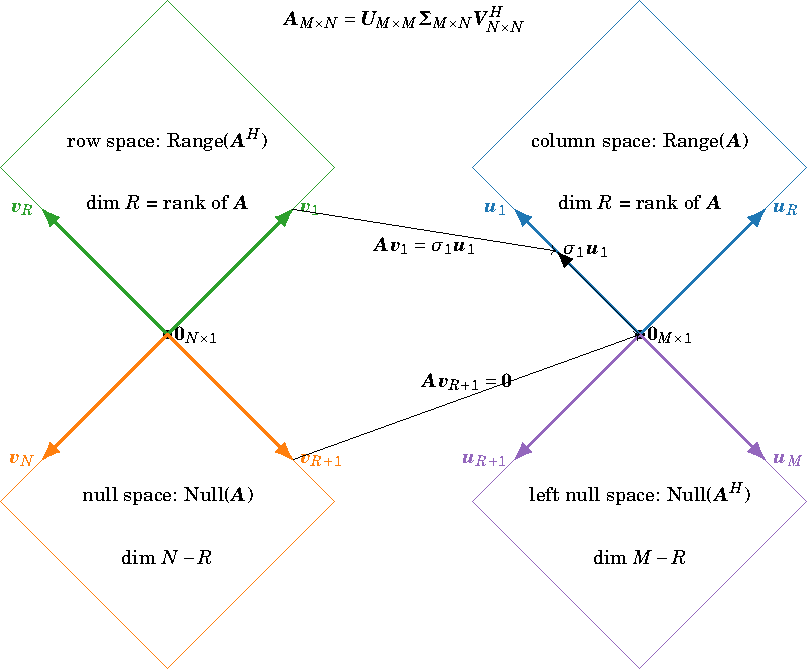
\includegraphics[width=0.5\textwidth]{four_subspaces.pdf}

\hspace{0.75cm}
right singular vectors in $\bm{V}$
\hspace{4.5cm}
left singular vectors in $\bm{U}$

\end{frame}




\begin{frame}{Projection Matrices Based on Left Inverse}
For full column rank $\bm{X}_{M \times N}$, rank $R=N$ the left inverse is
$$\bm{X}^{\dagger_l} = \bm{V} \bm{\Sigma}^{\dagger_l}\bm{U}^\mathrm{H} = (\bm{X}^\mathrm{H}\bm{X})^{-1} \bm{X}^\mathrm{H}$$
from which we can create \underline{four projection matrices} into the \underline{four subspaces}
\begin{itemize}
\item[-] into \textcolor{C2}{row space} $\bm{P}_\text{row} = \bm{X}^{\dagger_l} \bm{X} = \bm{I}_{N \times N}$ \begin{footnotesize}(i.e. the concept of a left inverse)\end{footnotesize}
\item[-] into \textcolor{C1}{null space} $\bm{P}_\text{null} = \bm{I} - \bm{P}_\text{row} = \bm{0}_{N \times N}$ \begin{footnotesize}(because no null space when full column rank)\end{footnotesize}
\item[-] into \textcolor{C0}{column space} $\bm{P}_\text{column} = (\bm{X} \bm{X}^{\dagger_l})_{M \times M}$ \begin{footnotesize}(very often called hat matrix)\end{footnotesize}
\item[-] into \textcolor{C4}{left nullspace} $\bm{P}_\text{left null} = \bm{I}_{M \times M} - \bm{P}_\text{column}$
\end{itemize}

Estimator $\hat{\bm{\theta}}$ from solving the inverse problem yields a vector $\hat{\bm{y}}$ living in the column space
$$\bm{X} \hat{\bm{\theta}} = \bm{X} (\bm{X}^{\dagger_l} \bm{y}) = \bm{P}_\text{column} \bm{y} = \hat{\bm{y}}$$
This means that there is a remaining part (typically called residual) $\bm{e}$ from measured $\bm{y}$
$$\bm{e} = \bm{y} - \hat{\bm{y}} = \bm{y} - \bm{P}_\text{column} \bm{y} = (\bm{I}_{M \times M} - \bm{P}_\text{column}) \bm{y}=
\bm{P}_\text{left null} \bm{y} = \bm{e}$$
which lives in the left null space. Due to the orthogonal subspaces, we know that $\hat{\bm{y}} \perp \bm{e}$.
\end{frame}




\begin{frame}[t]{Ex05: Matrix with Large Condition Number}
%Square matrix, full rank, thus invertible
$$
\bm{X}
=
\begin{bmatrix}
\sqrt{2} & \sqrt{2}\\
+\frac{\sqrt{2}}{100} & -\frac{\sqrt{2}}{100}
\end{bmatrix}
=
\bm{U} \bm{\Sigma} \bm{V}^H
=
\begin{bmatrix}
1 & 0\\
0 & 1
\end{bmatrix}
\begin{bmatrix}
\textcolor{C0}{2} & 0\\
0 & \textcolor{C1}{\frac{2}{100}}
\end{bmatrix}
\left(
\begin{bmatrix}
\frac{1}{\sqrt{2}} & \frac{1}{\sqrt{2}} \\
\frac{1}{\sqrt{2}} & -\frac{1}{\sqrt{2}}
\end{bmatrix}
\right)^H
$$
\pause
%
Left-inverse / here actually the Exact-inverse requires
$$\hat{\bm{\theta}} = \frac{\bm{u}_1^H \bm{y}}{\textcolor{C0}{\sigma_1}}\bm{v}_1 + \frac{\bm{u}_2^H \bm{y}}{\textcolor{C1}{\sigma_2}}\bm{v}_2$$
\pause
%
for $\bm{y}=[1,1]^T$ we get
$$\hat{\bm{\theta}} = \frac{1}{\textcolor{C0}{2}}\bm{v}_1 + \frac{1}{\textcolor{C1}{\frac{2}{100}}}\bm{v}_2 =
\frac{1}{\textcolor{C0}{2}}
\begin{bmatrix}
\frac{1}{\sqrt{2}}\\
\frac{1}{\sqrt{2}}
\end{bmatrix}
 + 50
\begin{bmatrix}
\frac{1}{\sqrt{2}}\\
\frac{1}{-\sqrt{2}}
\end{bmatrix}
\approx
\begin{bmatrix}
35.7089\\
-35.0018
\end{bmatrix}
$$
\pause
%
for $\bm{y}=[1 \pm \epsilon_1, 1 \pm \epsilon_2]^T$ we get
$$\hat{\bm{\theta}} =
\frac{1 \pm \epsilon_1}{\textcolor{C0}{2}}\bm{v}_1 +
\frac{1 \pm \epsilon_2}{\textcolor{C1}{\frac{2}{100}}}\bm{v}_2 =
\frac{1 \pm \epsilon_1}{\textcolor{C0}{2}}
\begin{bmatrix}
\frac{1}{\sqrt{2}}\\
\frac{1}{\sqrt{2}}
\end{bmatrix}
+ \textcolor{C3}{50} (1 \pm \textcolor{C3}{\epsilon_2})
\frac{}{}
\begin{bmatrix}
\frac{1}{\sqrt{2}}\\
\frac{1}{-\sqrt{2}}
\end{bmatrix}
$$




\end{frame}










\begin{frame}[t]{Ex05: Regularization of the LS-Problem}
$\cdot$ full column rank inverse problem $\rightarrow$ solve with left inverse $\bm{X}^{\dagger_l} \bm{y} = \bm{\theta}$
$$
\bm{X}^{\dagger_l}_{N \times M}
=
\bm{V}_{N \times N}\quad
\bm{\Sigma}^{\dagger_l}_{N \times M}\quad
(\bm{U}_{M \times M})^\mathrm{H}
=
\bm{V}
\begin{bmatrix}
\frac{\sigma_1}{\sigma_1^2} & 0 & 0 & 0 & 0 & 0\\
0 & \frac{\sigma_2}{\sigma_2^2} & 0 & 0 & 0 & 0\\
0 & 0 & \frac{\sigma_i}{\sigma_i^2} & 0 & 0 & 0\\
0 & 0 & 0 & \frac{\sigma_R}{\sigma_R^2} & 0 & 0
\end{bmatrix}
\bm{U}^\mathrm{H}
$$

$\cdot$ if condition number $\kappa(\bm{X}) = \frac{\sigma_\text{max}}{\sigma_\text{min}}$ is very large, regularization yields more robust solutions

$\cdot$ \textcolor{C0}{Tikhonov} regularization aka \textcolor{C0}{ridge regression} applies following modification

$$
\bm{\Sigma}^{\dagger_l} = (\bm{\Sigma}^H \bm{\Sigma})^{-1} \bm{\Sigma}^H \longrightarrow
\bm{\Sigma}^{\dagger_\text{ridge}} = (\bm{\Sigma}^H \bm{\Sigma} + \textcolor{C0}{\lambda \bm{I}})^{-1} \bm{\Sigma}^H
$$

$$
\bm{\Sigma}^{\dagger_\text{ridge}} =
\begin{bmatrix}
\frac{\sigma_1}{\sigma_1^2 + \textcolor{C0}{\lambda}} & 0 & 0 & 0 & 0 & 0\\
0 & \frac{\sigma_2}{\sigma_2^2 + \textcolor{C0}{\lambda}} & 0 & 0 & 0 & 0\\
0 & 0 & \frac{\sigma_i}{\sigma_i^2 + \textcolor{C0}{\lambda}} & 0 & 0 & 0\\
0 & 0 & 0 & \frac{\sigma_R}{\sigma_R^2 + \textcolor{C0}{\lambda}} & 0 & 0
\end{bmatrix}
$$
\end{frame}

\begin{frame}[t]{Ridge Regression as Regularization of the LS-Problem}
%\begin{center}
$
\bm{\Sigma}^{\dagger_\text{ridge}} =
\begin{bmatrix}
\frac{\sigma_1}{\sigma_1^2 + \textcolor{C0}{\lambda}} & 0 & 0 & 0 & 0 & 0\\
0 & \frac{\sigma_2}{\sigma_2^2 + \textcolor{C0}{\lambda}} & 0 & 0 & 0 & 0\\
0 & 0 & \frac{\sigma_i}{\sigma_i^2 + \textcolor{C0}{\lambda}} & 0 & 0 & 0\\
0 & 0 & 0 & \frac{\sigma_R}{\sigma_R^2 + \textcolor{C0}{\lambda}} & 0 & 0
\end{bmatrix}
$
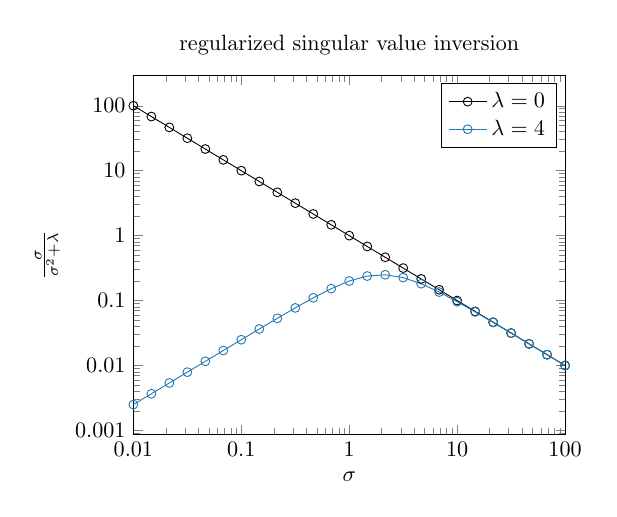
\begin{tikzpicture}[scale=0.8]
\begin{loglogaxis}
[xmin=1e-2, xmax=1e2, domain=1e-2:1e2,
log ticks with fixed point,
xlabel={$\sigma$},
ylabel={$\frac{\sigma}{\sigma^2 + \lambda}$},
title={regularized singular value inversion}]
\addplot[color=black, mark=o] {x / (x*x)};
\addlegendentry{$\lambda=0$}
\addplot[color=C0, mark=o] {x / (x*x + 4)};
\addlegendentry{$\lambda=4$}
\end{loglogaxis}
\end{tikzpicture}
%\end{center}
\end{frame}







\begin{frame}[t]{L-Curve to Find Optimum Regularization Parameter $\lambda$}
$$
\hat{\bm{\theta}}(\textcolor{C0}{\lambda}) \quad=\quad
\left[\bm{V} (\bm{\Sigma}^\mathrm{H} \bm{\Sigma} + \textcolor{C0}{\lambda}\bm{I})^{-1} \bm{\Sigma}^\mathrm{H} \bm{U}^\mathrm{H}\right] \bm{y} \quad=\quad
\left[(\bm{X}^\mathrm{H}\bm{X} + \textcolor{C0}{\lambda}\bm{I})^{-1} \bm{X}^\mathrm{H}\right] \bm{y}
$$
\begin{center}
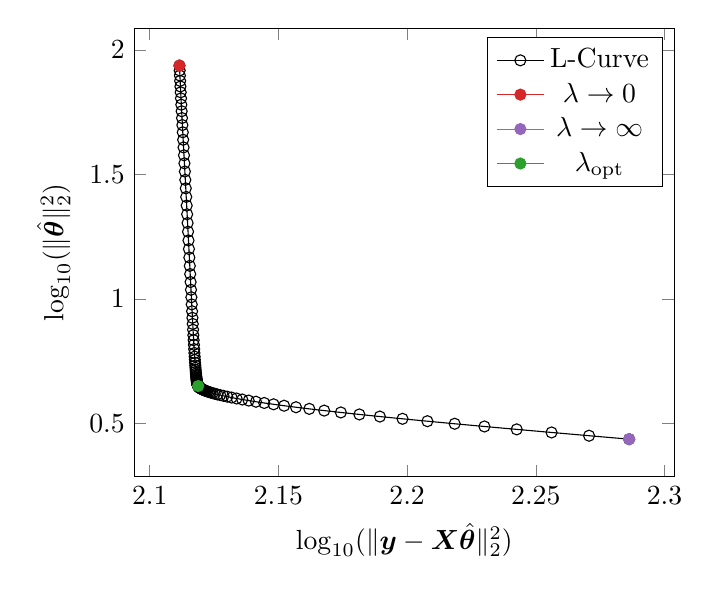
\begin{tikzpicture}[scale=1]
\begin{axis}
[
xlabel={$\log_{10}(\lVert \bm{y} - \bm{X}\hat{\bm{\theta}}\rVert_2^2)$},
ylabel={$\log_{10}(\lVert \hat{\bm{\theta}}\rVert_2^2)$}]
\addplot[mark=o, color=black]
coordinates {(2.111535073672359,1.9374862138307345)(2.1116189173400763,1.9179406901143072)(2.1117093198996537,1.8974485918662078)(2.1118064331906368,1.8759963319337574)(2.111910359738582,1.8535739649613479)(2.1120211470508305,1.830175603962491)(2.112138782658966,1.8057998415008494)(2.1122631901246884,1.7804501723459156)(2.112394226206225,1.7541354143971832)(2.112531679351133,1.7268701245749452)(2.112675269639379,1.6986750062035103)(2.1128246502497285,1.6695773040966553)(2.112979410465293,1.639611183016149)(2.1131390801738505,1.6088180843238344)(2.1133031357587573,1.5772470543949442)(2.1134710072206198,1.544955036620565)(2.113642086321722,1.5120071165358628)(2.1138157355074134,1.478476706741184)(2.1139912973332855,1.4444456548692113)(2.1141681041151705,1.410004254014596)(2.1143454875209553,1.37525113102209)(2.114522787838079,1.340292984210847)(2.1146993626767765,1.3052441390503273)(2.1148745949043666,1.270225888724319)(2.1150478996474744,1.2353655873001401)(2.115218730244241,1.2007954673176384)(2.115386583074499,1.1666511619432884)(2.115551001240152,1.1330699250899565)(2.115711577108509,1.1001885613165483)(2.1158679537665215,1.068141100418087)(2.11601982546278,1.037056277997946)(2.1161669371362017,1.007054910564738)(2.116309083145609,0.9782472784885935)(2.1164461053231896,0.9507306486073885)(2.1165778904778176,0.9245870765849667)(2.1167043674722255,0.8998816243422154)(2.1168255039920445,0.87666110870323)(2.1169413031156927,0.8549534647147454)(2.1170517997829794,0.8347677641141822)(2.117157057247913,0.8160948812415754)(2.117257163588327,0.7989087514113858)(2.1173522283321478,0.7831681263140827)(2.1174423792479082,0.7688187020534032)(2.117527759335815,0.7557954805263869)(2.1176085240455236,0.7440252242668157)(2.117684838737914,0.7334288767631709)(2.117756876400629,0.7239238413513156)(2.117824815620946,0.7154260381552079)(2.1178888388146193,0.7078516864121741)(2.117949130705606,0.7011187857530566)(2.118005877048923,0.6951482924562146)(2.1180592635871736,0.6898650042082011)(2.1181094752304657,0.6851981792042556)(2.118156695449283,0.6810819228711115)(2.118201105870427,0.6774553788469092)(2.118242886067188,0.6742627610332226)(2.1182822135364323,0.671453261473149)(2.1183192638572503,0.6689808653381029)(2.118354211028092,0.6668041001025019)(2.1183872279819753,0.6648857415608906)(2.1184184872823195,0.6631924950508753)(2.118448162005227,0.6616946663102274)(2.1184764268176903,0.6603658329371096)(2.1185034592651766,0.6591825244830672)(2.118529441286444,0.6581239167829298)(2.118554560978318,0.6571715441765998)(2.1185790146385304,0.6563090317506081)(2.1186030091207133,0.6555218485615588)(2.1186267645423507,0.6547970819385508)(2.1186505173939523,0.654123232340967)(2.1186745241061593,0.6534900278214899)(2.1186990651409325,0.6528882568688616)(2.118724449683664,0.6523096182447616)(2.1187510210250817,0.651746586354894)(2.1187791627354,0.6511922906824332)(2.11880930574847,0.6506404078438874)(2.1188419364909588,0.6500850648888835)(2.1188776062109627,0.6495207525455089)(2.118916941682254,0.6489422472035514)(2.118960657484724,0.6483445405233506)(2.1190095700887626,0.6477227756537961)(2.119064614001517,0.6470721891364337)(2.119126860266296,0.6463880576617214)(2.1191975376430543,0.6456656489271558)(2.1192780568377905,0.6449001759246437)(2.119370038191856,0.6440867540559502)(2.1194753432882476,0.6432203605404804)(2.1195961109805195,0.6422957956393021)(2.119734798400172,0.6413076452737028)(2.1198942275491164,0.6402502446661995)(2.120077638133322,0.63911764267742)(2.1202887473397256,0.6379035665542551)(2.1205318172976866,0.636601386843793)(2.120811730994491,0.635204082264455)(2.1211340774261433,0.6337042043610798)(2.1215052467528444,0.6320938418050998)(2.1219325361842487,0.6303645842350503)(2.1224242672317533,0.628507485567048)(2.122989914820136,0.6265130267401864)(2.1236402485326384,0.6243710778985797)(2.124387485952922,0.622070860050626)(2.1252454576423543,0.6196009062874555)(2.126229782727388,0.6169490226869792)(2.127358053343277,0.6141022490778995)(2.128650025260821,0.6110468198898391)(2.1301278108879216,0.6077681253716871)(2.131816069468935,0.6042506735205079)(2.1337421876938722,0.6004780531279676)(2.1359364420852347,0.5964328984200181)(2.138432132486612,0.5920968558382564)(2.1412656738028524,0.5874505535872641)(2.144476630950979,0.5824735746505099)(2.148107679944085,0.5771444340567427)(2.152204476381007,0.571440561257629)(2.1568154116529623,0.5653382885535984)(2.1619912372646763,0.5588128465759031)(2.1677845392020596,0.551838367895746)(2.1742490476635825,0.5443878998824194)(2.181438773054784,0.5364334279677112)(2.189406967138293,0.5279459104888987)(2.1982049186248642,0.5188953262726451)(2.2078806049594526,0.5092507360820187)(2.2184772358913527,0.4989803589736009)(2.230031738502925,0.48805166449639775)(2.2425732462333383,0.476431481504676)(2.2561216643783273,0.4640861241494426)(2.2706863898872727,0.4509815353558515)(2.2862652626236226,0.4370834477858121)};
\addlegendentry{L-Curve}
%
\addplot[color=C3, mark=*, mark options={fill=C3}]
coordinates {(2.111535073672359,1.9374862138307345)};
\addlegendentry{$\lambda \rightarrow 0$}
%
\addplot[color=C4, mark=*, mark options={fill=C4}]
coordinates {(2.2862652626236226,0.4370834477858121)};
\addlegendentry{$\lambda \rightarrow \infty$}
%
\addplot[color=C2, mark=*, mark options={fill=C2}]
coordinates {(2.11880930574847,0.6506404078438874)};
\addlegendentry{$\lambda_\text{opt}$}
%
\end{axis}
\end{tikzpicture}
\end{center}
\end{frame}


















\begin{frame}[t]{Linear Regression}
Both optimization problems,

$\cdot$ the Least Squares Error Problem with Tikhonov Regularization (aka Ridge Regression)
$$
\min_{\text{wrt }\bm{\theta}} J(\bm{\theta}) \quad\text{with cost function}\quad
J(\bm{\theta}) =
\lVert\bm{y} - \bm{X} \bm{\theta}\rVert_2^2 + \textcolor{C0}{\lambda} \lVert \bm{\theta} \rVert_2^2
$$

$\cdot$ and the plain Least Squares Error Problem (i.e. for $\textcolor{C0}{\lambda}=0$)
$$
\min_{\text{wrt }\bm{\theta}} J(\bm{\theta}) \quad\text{with cost function}\quad
J(\bm{\theta}) =  \lVert\bm{y} - \bm{X} \bm{\theta}\rVert_2^2
$$

have the closed form solution using the (regularized) left inverse of $\bm{X} = \bm{U}\bm{\Sigma}\bm{V}^H$:
$$
\hat{\bm{\theta}} \quad=\quad
\left[\bm{V} (\bm{\Sigma}^\mathrm{H} \bm{\Sigma} + \textcolor{C0}{\lambda \bm{I})}^{-1} \bm{\Sigma}^\mathrm{H} \bm{U}^\mathrm{H}\right] \bm{y} \quad=\quad
\left[(\bm{X}^\mathrm{H}\bm{X} + \textcolor{C0}{\lambda \bm{I}})^{-1} \bm{X}^\mathrm{H}\right] \bm{y}
$$

Such a model has $N$ \underline{model parameters} $\bm{\theta} = [\theta_1, \theta_2 \dots \theta_N]^T$ and one \underline{hyper parameter} $\textcolor{C0}{\lambda}$ to be learned from the data $\bm{y}_{M \times 1}$ and the feature matrix $\bm{X}_{M \times N}$ with full column rank $R=N$.

\end{frame}




\begin{frame}[t]{Ex06: Audio Toy Example for Linear Regression and SVD}
\begin{center}
$
\def\L{0.5}
\def\F{1}
\def\N{3}
\def\rank{0.999999}
\drawmatrix[fill=none, height=\N, width=0]{y}_\mathtt{N \times 1} =
\drawmatrix[fill=none, height=\N, width=\F]{X}_\mathtt{N \times F}
\drawmatrix[fill=none, height=\F, width=0]\theta_\mathtt{F \times 1}+
\drawmatrix[fill=none, height=\N, width=0]{\nu}_\mathtt{N \times 1}
=
\drawmatrix[bbox style={fill=C4}, bbox height=\N, bbox width=\N, fill=C0, height=\N, width=\rank\F]U_\mathtt{N \times N}
\drawmatrix[bbox style={fill=gray!50}, bbox height=\N, bbox width=\F, fill=white, height=\rank\F, width=\rank\F]\Sigma_\mathtt{N \times F}
\drawmatrix[bbox style={fill=C1}, bbox height=\F, bbox width=\F, fill=C2, height=\F, width=\rank\F]{V}_\mathtt{F \times F}^H
\drawmatrix[fill=none, height=\F, width=0]\theta_\mathtt{F \times 1}+
\drawmatrix[fill=none, height=\N, width=0]{\nu}_\mathtt{N \times 1}
$
\end{center}
\end{frame}



\begin{frame}{Ex06: Audio Toy Example for Linear Regression and SVD}
Consider the following linear combinations
$$\bm{X} \bm{\theta} + \bm{\nu} = \bm{y}$$
where $\bm{\theta}=[\theta_1, \theta_2, \theta_3, ..., \theta_{F}]^\mathrm{T}$ are typical variables for the model parameter vector.
%
\begin{itemize}
\item $\bm{X}_{N \times F}$ matrix with $N$ audio samples for each column, $f$-th column represents the $f$-th audiotrack / feature
\item $\bm{\theta}_{F \times 1}$ column vector of scalar values that represent a dedicated gain for each audiotrack
\item $\bm{\nu}_{N \times 1}$ column vector that represents an $N$-sample long noise signal added to the mixdown $\bm{X} \bm{\theta}$
\item $\bm{y}_{N \times 1}$ audio signal with $N$ samples as a result of the linear model's linear combination plus noise
\end{itemize}
%
Let us assume that a) we know $\bm{X}$ (i.e. the individual audio tracks) and $\bm{y}$ (i.e. the noise-corrupted final mixdown), b) that we do not know the noise $\bm{n}$ and c) that we want to estimate the 'real world' mixing gains $\bm{\theta}$
\end{frame}



\section{Section II: Feature Design}

\begin{frame}[t]{Ex07: Audio Features}
no slides so far
\end{frame}


\begin{frame}[t]{Ex08: Principal Component Analysis (PCA)}

PCA is typically applied on mean-free data

$\cdot$ for an $N \times F$ full-column rank matrix $\bm{X}$ we ensure that each column is mean-free by
$$\bm{X}_{N \times F} \leftarrow \bm{X}_{N \times F} - \frac{1}{N} \bm{1}_{N \times N} \bm{X}_{N \times F}$$

$\cdot$ for an $F \times N$ full-row rank matrix $\bm{X}$ we ensure that each row is mean-free by
$$\bm{X}_{F \times N} \leftarrow \bm{X}_{F \times N} - \frac{1}{N} \bm{X}_{F \times N} \bm{1}_{N \times N}$$

PCA is often additionally performed on unit-variance preprocessed data, cf. function zscore()

this then yields a total variance of $$\mathrm{trace}(\mathrm{cov}(\mathrm{zscore}(\bm{X})))= F$$

which the PCA spreads over the principal component (PC) scores

\end{frame}



\begin{frame}[t]{Ex08: Principal Component Analysis (PCA) via SVD}

$\cdot$ for $\bm{X}_c \in\mathbb{R}$, $\bm{X}_c = \bm{X}_r^\mathrm{T}$, $\bm{F}_c = \bm{F}_r^\mathrm{T}$, SVD matrices $\bm{U} \bm{\Sigma} \bm{V}^\mathrm{T}$ for $\bm{X}_c$

$\cdot$ PC scores are ortho\underline{gonal} and variance-sorted, PC loadings are ortho\underline{normal}

\vspace{0.5em}
\begin{minipage}[t]{0.49\textwidth}
full-column rank, mean-free columns
\begin{center}
$
\def\F{0.5}
\def\N{2}
\drawmatrix[fill=none, height=\N, width=\F]{X_{c}}_\mathtt{N \times F}
=
\drawmatrix[fill=C0, height=\N, width=\F]{F_{c}}_\mathtt{N \times F}
\drawmatrix[fill=C2, height=\F, width=\F]{L}_\mathtt{F \times F}^\mathrm{T}
$
\end{center}
\end{minipage}
%
\begin{minipage}[t]{0.49\textwidth}
full-row rank, mean-free rows
\begin{center}
$
\def\F{0.5}
\def\N{2}
\drawmatrix[fill=none, height=\F, width=\N]{X_{r}}_\mathtt{F \times N}
=
\drawmatrix[fill=C0, height=\F, width=\F]{L}_\mathtt{F \times F}
\drawmatrix[fill=C2, height=\F, width=\N]{F_{r}}_\mathtt{F \times N}
$
\end{center}
\end{minipage}

\begin{minipage}[t]{0.49\textwidth}

Mapping

$\bm{X}_c= \bm{U} \bm{\Sigma} \bm{V}^\mathrm{T} = \bm{F}_c \bm{L}^\mathrm{T}$

$\bm{F}_c = \bm{X}_c \bm{L} = \bm{X}_c \bm{V} = \bm{U} \bm{\Sigma}$

PC scores $\bm{F}_c =
\begin{bmatrix}
| & | & | & |\\
\bm{f}_1 & \bm{f}_2 & : & \bm{f}_F\\
| & | & | & |\\
\end{bmatrix}
= \bm{U} \bm{\Sigma}$

PC loadings $\bm{L} = \bm{V}$


\end{minipage}
%
\begin{minipage}[t]{0.49\textwidth}

Mapping

$\bm{X}_r = \bm{V} \bm{\Sigma} \bm{U}^\mathrm{T} = \bm{L} \bm{F}_r$

$\bm{F}_r = \bm{L}^\mathrm{T} \bm{X}_r = \bm{V}^\mathrm{T} \bm{X}_r = \bm{\Sigma} \bm{U}^\mathrm{T}$

PC scores $\bm{F}_r =
\begin{bmatrix}
- \bm{f}_1 -\\
- \bm{f}_2 -\\
- : -\\
- \bm{f}_F -
\end{bmatrix}
=
\bm{\Sigma} \bm{U}^\mathrm{T}$

PC loadings $\bm{L} = \bm{V} $



\end{minipage}

\end{frame}







\begin{frame}[t]{Ex08: Principal Component Analysis (PCA) via Covariance}

$\cdot$ for $\bm{X}_c \in\mathbb{R}$, $\bm{X}_c = \bm{X}_r^\mathrm{T}$, $\bm{F}_c = \bm{F}_r^\mathrm{T}$, SVD matrices $\bm{U} \bm{\Sigma} \bm{V}^\mathrm{T}$ for $\bm{X}_c$

$\cdot$ PC scores are ortho\underline{gonal} and variance-sorted, PC loadings are ortho\underline{normal}

\vspace{0.5em}
\begin{minipage}[t]{0.49\textwidth}
full-column rank, mean-free columns
\begin{center}
$
\def\F{0.5}
\def\N{2}
\drawmatrix[fill=none, height=\N, width=\F]{X_{c}}_\mathtt{N \times F}
=
\drawmatrix[fill=C0, height=\N, width=\F]{F_{c}}_\mathtt{N \times F}
\drawmatrix[fill=C2, height=\F, width=\F]{L}_\mathtt{F \times F}^\mathrm{T}
$
\end{center}
\end{minipage}
%
\begin{minipage}[t]{0.49\textwidth}
full-row rank, mean-free rows
\begin{center}
$
\def\F{0.5}
\def\N{2}
\drawmatrix[fill=none, height=\F, width=\N]{X_{r}}_\mathtt{F \times N}
=
\drawmatrix[fill=C0, height=\F, width=\F]{L}_\mathtt{F \times F}
\drawmatrix[fill=C2, height=\F, width=\N]{F_{r}}_\mathtt{F \times N}
$
\end{center}
\end{minipage}

\vspace{0.5em}

\begin{minipage}[t]{0.49\textwidth}
covariance matrix $\bm{C}_X = \frac{1}{N-1}\bm{X}_c^\mathrm{T}\bm{X}_c$

diagonalization (with SVD) $\bm{C}_X = \bm{V} \bm{\Lambda} \bm{V}^\mathrm{T}$

PC scores $\bm{F}_c = \bm{X}_c \bm{V}$

PC loadings $\bm{L} = \bm{V}$

\end{minipage}
%
\begin{minipage}[t]{0.49\textwidth}
covariance matrix $\bm{C}_X = \frac{1}{N-1}\bm{X}_r\bm{X}_r^\mathrm{T}$

diagonalization (with SVD) $\bm{C}_X = \bm{V} \bm{\Lambda} \bm{V}^\mathrm{T}$

PC scores $\bm{F}_r = \bm{V}^\mathrm{T} \bm{X}_r$

PC loadings $\bm{L} = \bm{V}$

\end{minipage}

\vspace{0.5em}

%\small
$\cdot$ an SVD-based diagonalization inherently sorts the eigenvalues in $\bm{\Lambda}$, making the orthogonal PC scores \underline{variance-sorted} (i.e. covariance matrix of $\bm{F}$ is a sorted diagonal matrix)

$\cdot$ $\bm{F} / \bm{L}$ might exhibit reflections compared to $\bm{F} / \bm{L}$ from SVD-based approach

$\cdot$ SVD / covariance approaches are consistent by itself as calculation of $\bm{F}$ and $\bm{L}$ is linked

\end{frame}



\begin{frame}[t]{Ex08: Principal Component Analysis (PCA) Feature Representation}

$\cdot$ for $\bm{X}_c \in\mathbb{R}$, $\bm{X}_c = \bm{X}_r^\mathrm{T}$, $\bm{F}_c = \bm{F}_r^\mathrm{T}$, SVD matrices $\bm{U} \bm{\Sigma} \bm{V}^\mathrm{T}$ for $\bm{X}_c$

\begin{minipage}[t]{0.49\textwidth}
full-column rank, mean-free columns

$\bm{X}_{c,N \times F}$

PC scores $\bm{F}_c = \bm{X}_c \bm{V}$

PC loadings $\bm{L} = \bm{V}$

\end{minipage}
%
\begin{minipage}[t]{0.49\textwidth}
full-row rank, mean-free rows

$\bm{X}_{r,F \times N}$

PC scores $\bm{F}_r = \bm{V}^\mathrm{T} \bm{X}_r$

PC loadings $\bm{L} = \bm{V}$

\end{minipage}

\vspace{1em}

Reduced PC loading matrix
$\bm{V}_K =
\begin{bmatrix}
| & | & |\\
\bm{v}_1 & : & \bm{v}_{K \leq F}\\
| & | & |\\
\end{bmatrix}
$
allows for the following techniques

\vspace{1em}

$\cdot$ Low-Rank Approximation / Truncated SVD (yields a matrix with lower rank $K$)

\begin{minipage}[t]{0.49\textwidth}

$\tilde{\bm{X}}_{c,N \times F} = (\bm{X}_c \bm{V}_K) \bm{V}_K^\mathrm{T} = \sum_{i=1}^{K} \sigma_i \bm{u}_i \bm{v}_i^\mathrm{T}$

\end{minipage}
%
\begin{minipage}[t]{0.49\textwidth}

$\tilde{\bm{X}}_{r,F \times N} = \bm{V}_K (\bm{V}_K^\mathrm{T} \bm{X}_r) = \sum_{i=1}^{K} \sigma_i \bm{v}_i \bm{u}_i^\mathrm{T}$

\end{minipage}

\vspace{1em}

$\cdot$ Linear Dimensionality Reduction (yields a matrix with smaller dimension $K$)

\begin{minipage}[t]{0.49\textwidth}
$\tilde{\bm{X}}_{c,N \times K} = \bm{X}_c \bm{V}_K =
\begin{bmatrix}
| & | & |\\
\bm{f}_1 & : & \bm{f}_{K}\\
| & | & |\\
\end{bmatrix}
$

i.e. take only first $K$ columns of $\bm{F}_c$
\end{minipage}
%
\begin{minipage}[t]{0.49\textwidth}
$\tilde{\bm{X}}_{r,K \times N} = \bm{V}_K^\mathrm{T} \bm{X}_r
=
\begin{bmatrix}
- \bm{f}_1 -\\
- : -\\
- \bm{f}_K -
\end{bmatrix}
$

i.e. take only first $K$ rows of $\bm{F}_r$
\end{minipage}

\end{frame}






\begin{frame}[t]{Ex08: Principal Component Analysis (PCA) 2D-Data Example}
\begin{minipage}[t]{0.49\textwidth}
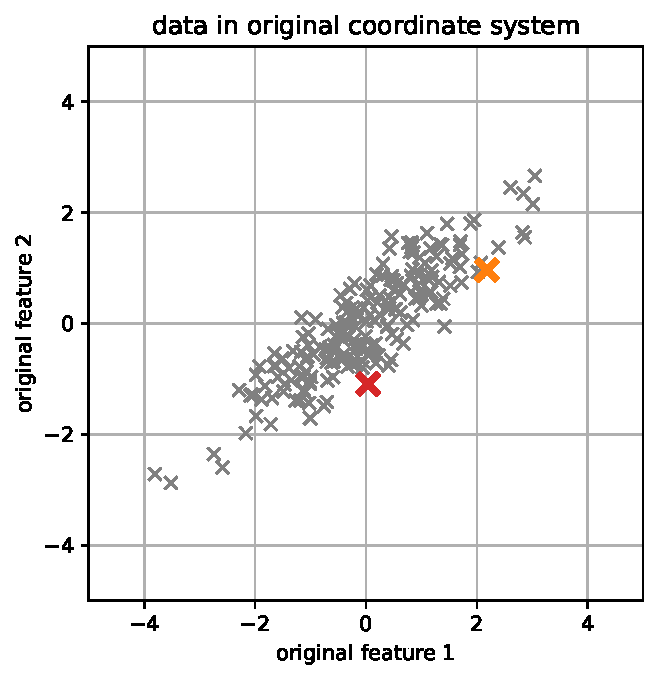
\includegraphics[width=\textwidth]{pca_2d_original_data.pdf}
\end{minipage}
%
\begin{minipage}[t]{0.49\textwidth}
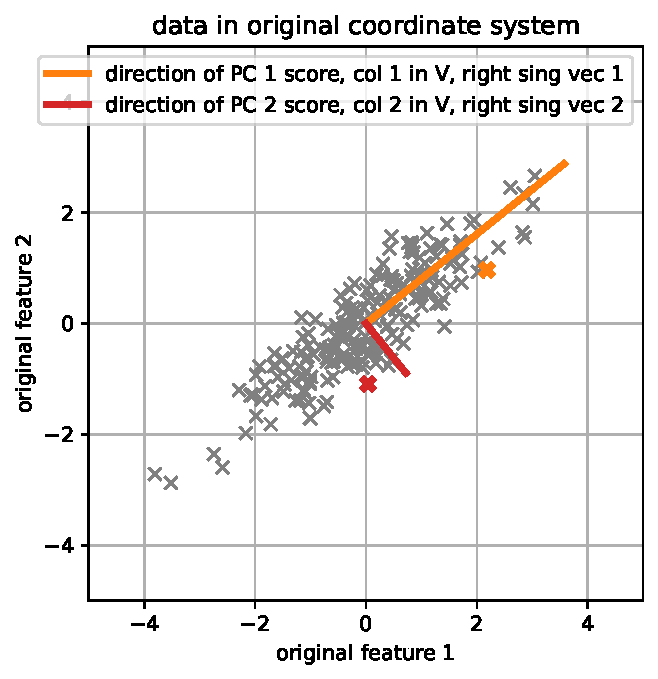
\includegraphics[width=\textwidth]{pca_2d_original_data_with_pcdir.pdf}
\end{minipage}
\end{frame}
%%
\begin{frame}[t]{Ex08: Principal Component Analysis (PCA) 2D-Data Example}
\begin{minipage}[t]{0.49\textwidth}
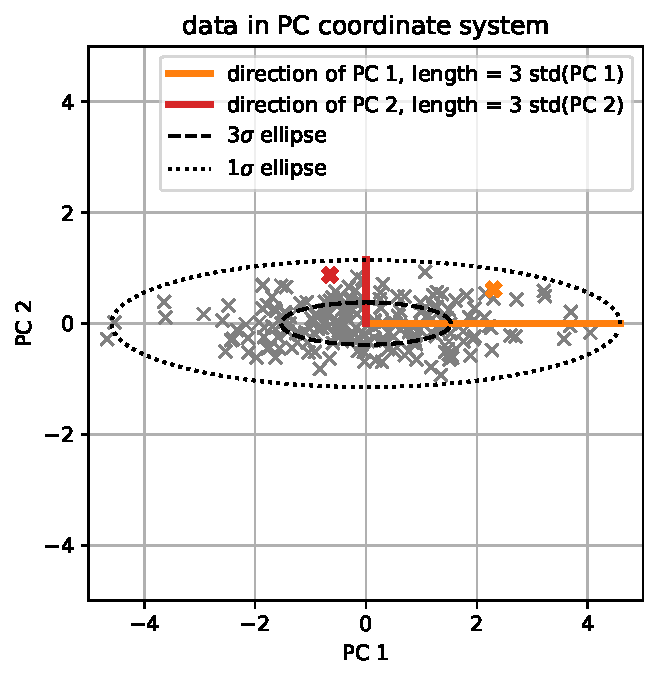
\includegraphics[width=\textwidth]{pca_2d_pc_data.pdf}
\end{minipage}
%
\begin{minipage}[t]{0.49\textwidth}
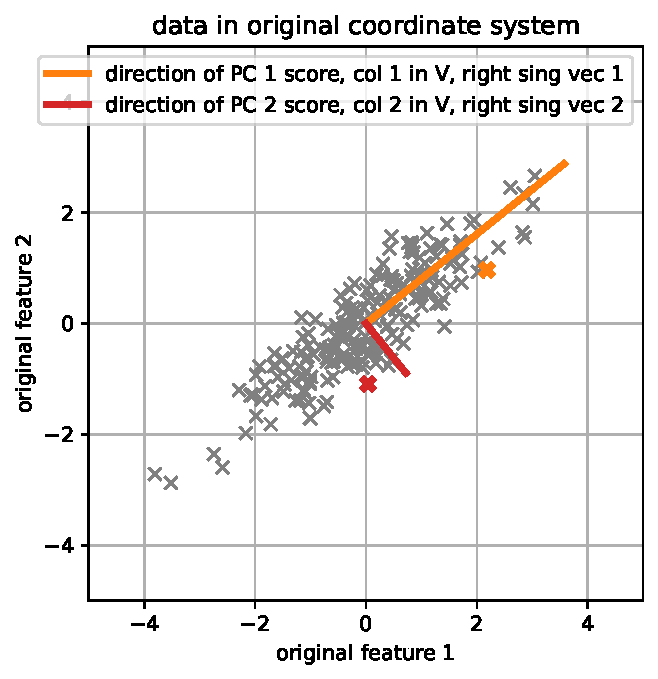
\includegraphics[width=\textwidth]{pca_2d_original_data_with_pcdir.pdf}
\end{minipage}
\end{frame}
%%
\begin{frame}[t]{Ex08: Principal Component Analysis (PCA) 2D-Data Example}
\begin{minipage}[t]{0.49\textwidth}
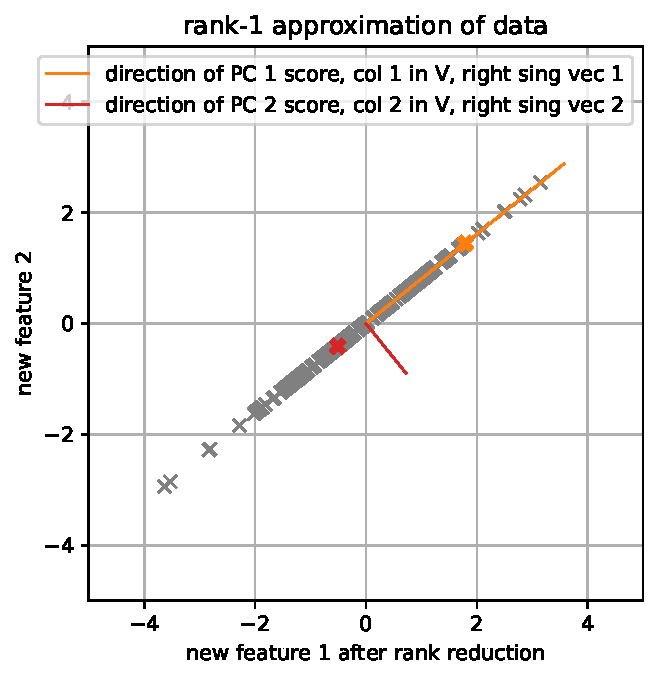
\includegraphics[width=\textwidth]{pca_2d_truncated_svd.pdf}
\end{minipage}
%
\begin{minipage}[t]{0.49\textwidth}
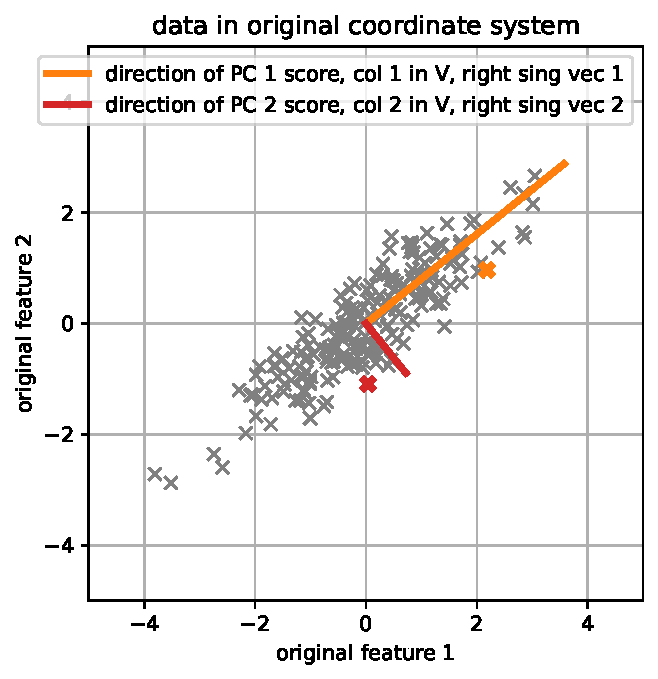
\includegraphics[width=\textwidth]{pca_2d_original_data_with_pcdir.pdf}
\end{minipage}
\end{frame}
%%
\begin{frame}[t]{Ex08: Principal Component Analysis (PCA) 2D-Data Example}
\begin{minipage}[t]{0.49\textwidth}
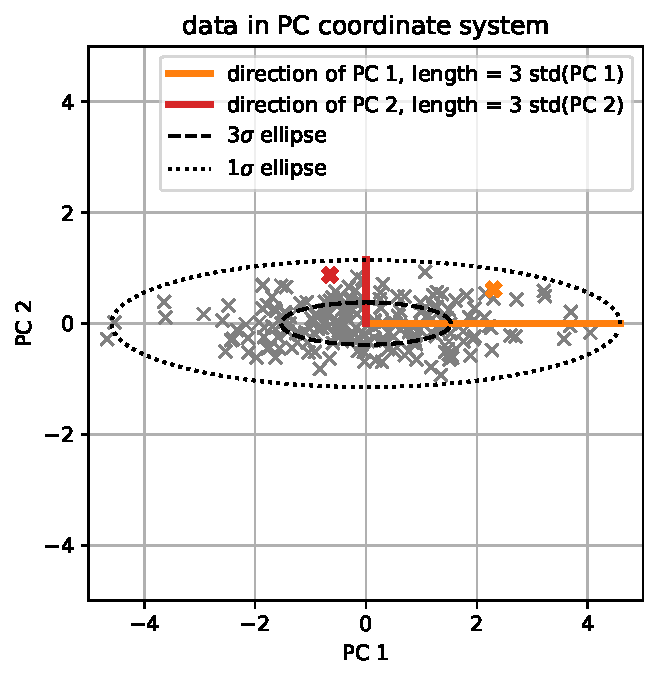
\includegraphics[width=\textwidth]{pca_2d_pc_data.pdf}
\end{minipage}
%
\begin{minipage}[t]{0.49\textwidth}
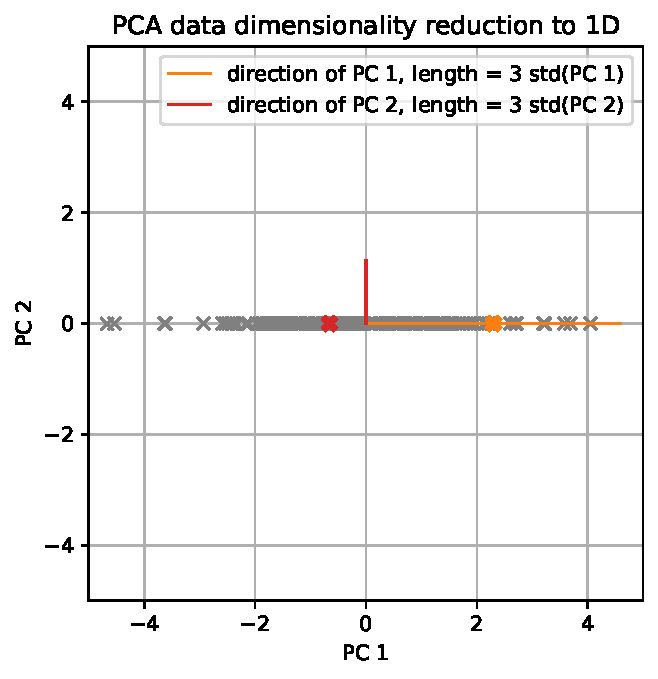
\includegraphics[width=\textwidth]{pca_2d_dim_red.pdf}
\end{minipage}
\end{frame}







\begin{frame}[t]{Ex08: Principal Component Analysis (PCA) 3D-Data Example}
\begin{minipage}[t]{0.49\textwidth}
original data cloud in 3D space

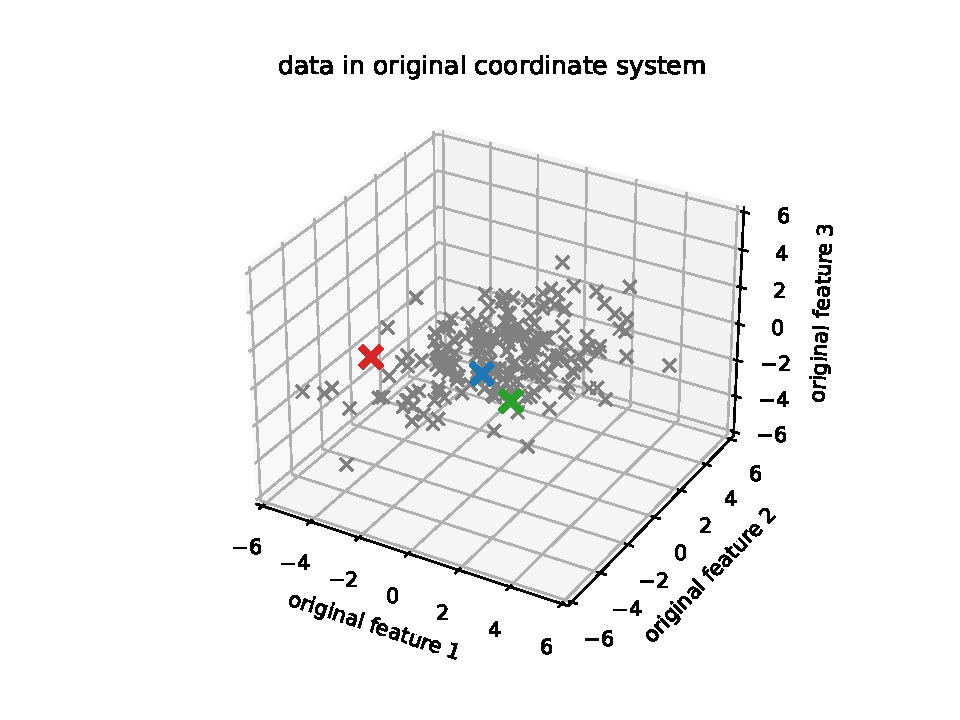
\includegraphics[width=\textwidth]{pca_3d_original_data.pdf}
\end{minipage}
%
\begin{minipage}[t]{0.49\textwidth}
original data cloud in 3D space

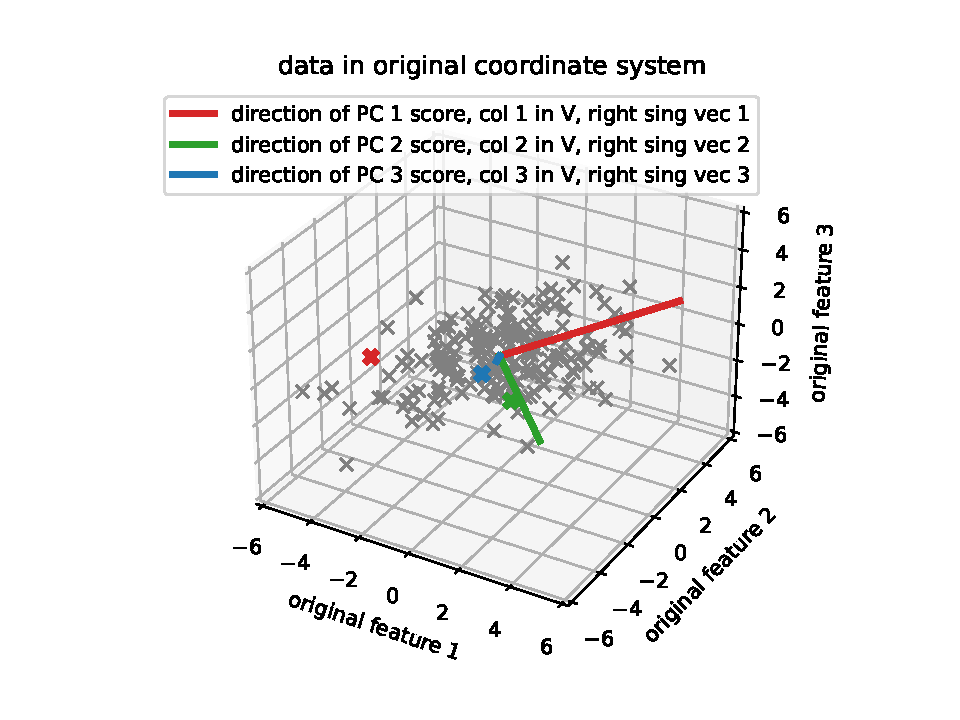
\includegraphics[width=\textwidth]{pca_3d_original_data_with_pcdir.pdf}
\end{minipage}
\end{frame}
%%
\begin{frame}[t]{Ex08: Principal Component Analysis (PCA) 3D-Data Example}
\begin{minipage}[t]{0.49\textwidth}
PC data cloud in 3D  space

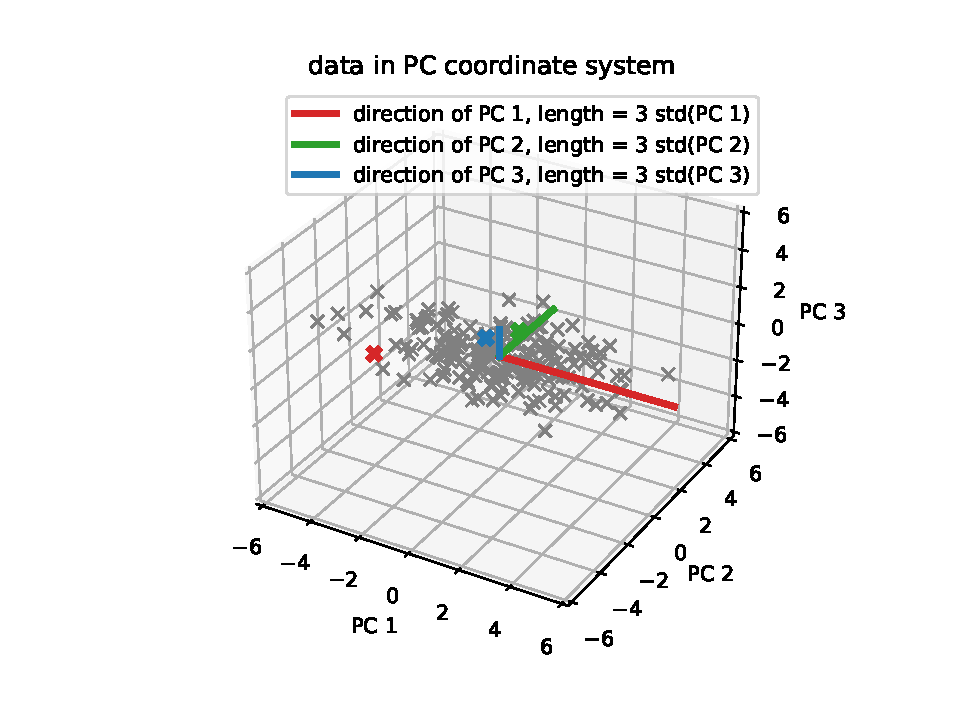
\includegraphics[width=\textwidth]{pca_3d_pc_data.pdf}
\end{minipage}
%
\begin{minipage}[t]{0.49\textwidth}
original data cloud in 3D space

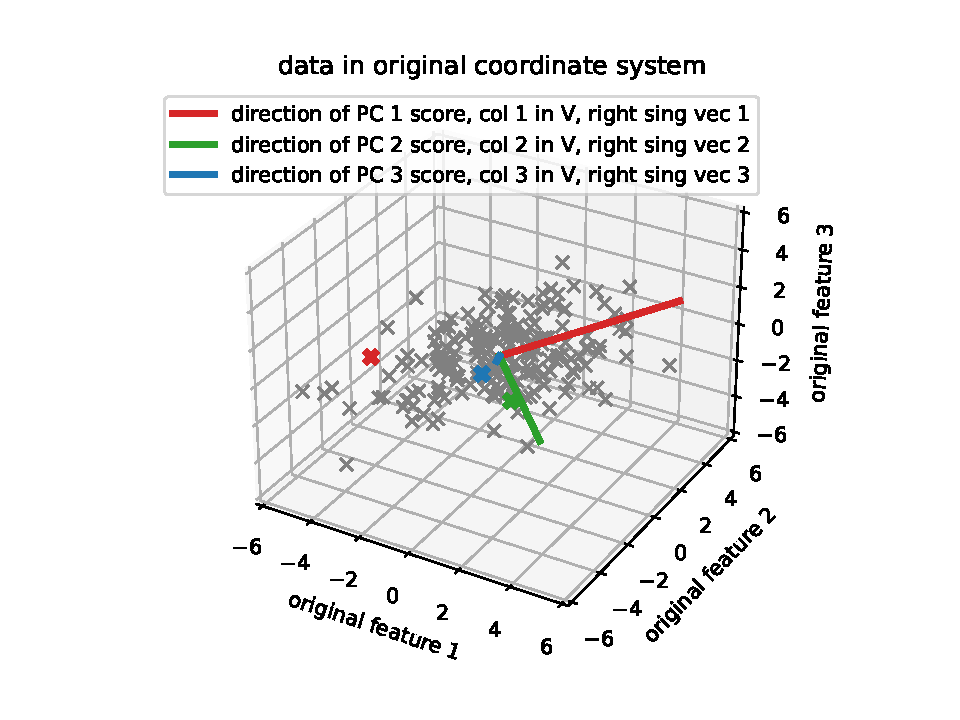
\includegraphics[width=\textwidth]{pca_3d_original_data_with_pcdir.pdf}
\end{minipage}
\end{frame}
%%
\begin{frame}[t]{Ex08: Principal Component Analysis (PCA) 3D-Data Example}
\begin{minipage}[t]{0.49\textwidth}
data \underline{plane} in 3D space

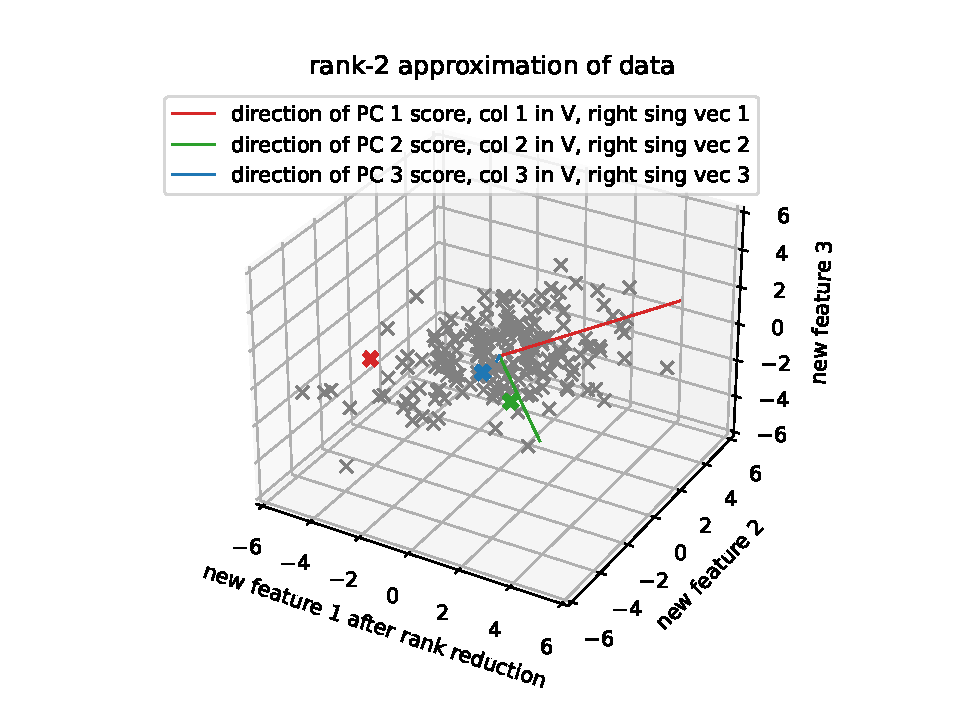
\includegraphics[width=\textwidth]{pca_3d_truncated_svd.pdf}
\end{minipage}
%
\begin{minipage}[t]{0.49\textwidth}
data cloud in 3D space

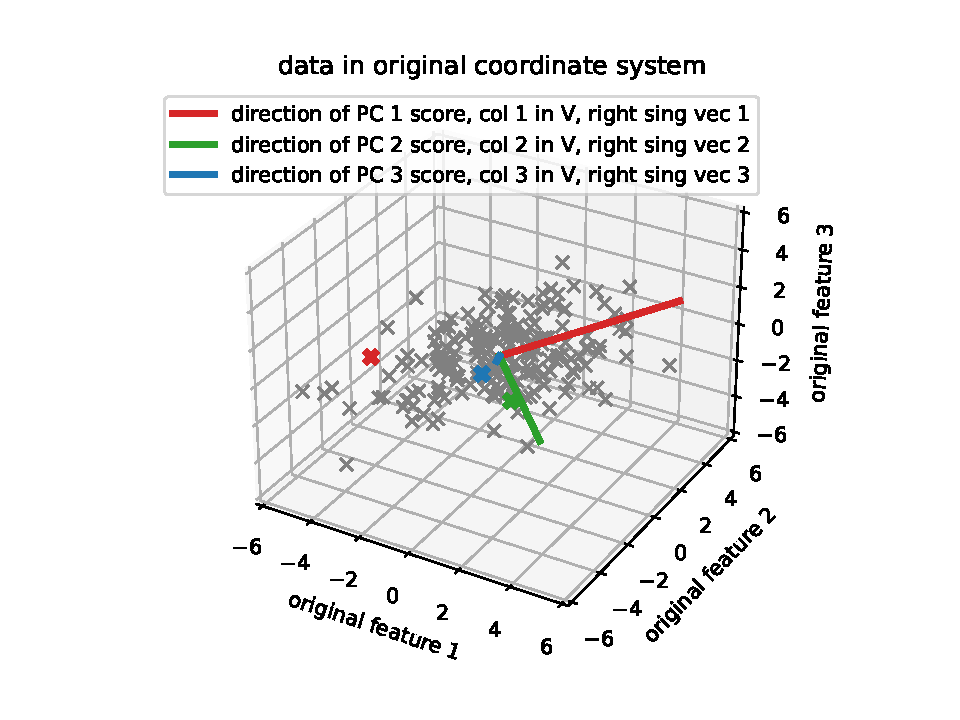
\includegraphics[width=\textwidth]{pca_3d_original_data_with_pcdir.pdf}
\end{minipage}
\end{frame}
%%
\begin{frame}[t]{Ex08: Principal Component Analysis (PCA) 3D-Data Example}
\begin{minipage}[t]{0.49\textwidth}
data cloud in 3D space

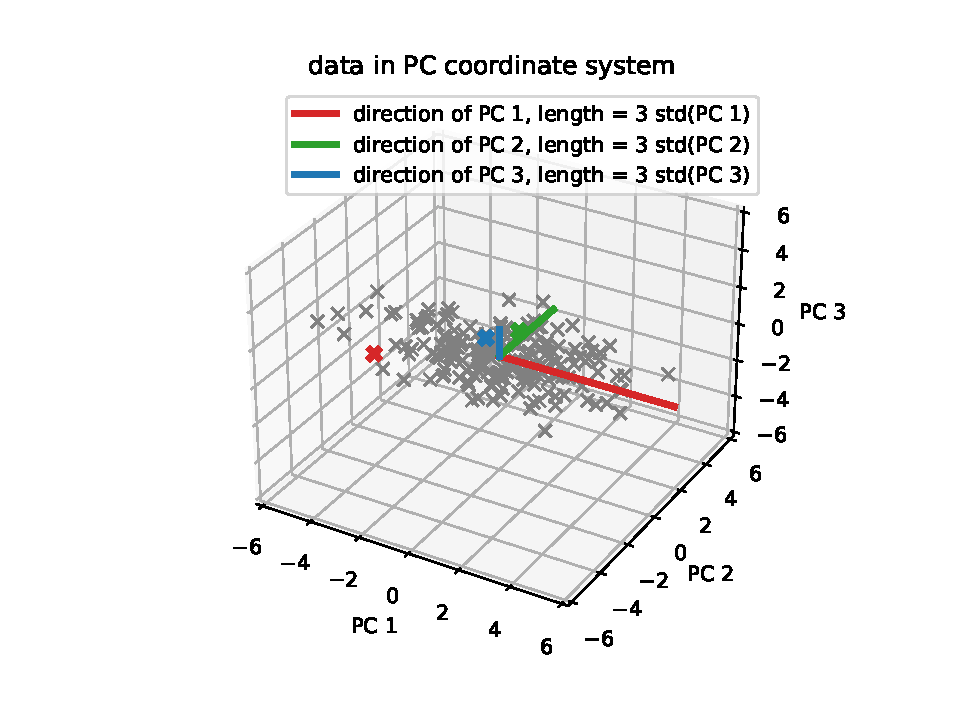
\includegraphics[width=\textwidth]{pca_3d_pc_data.pdf}
\end{minipage}
%
\begin{minipage}[t]{0.49\textwidth}
data \underline{plane} in 2D space (PC3 not used)

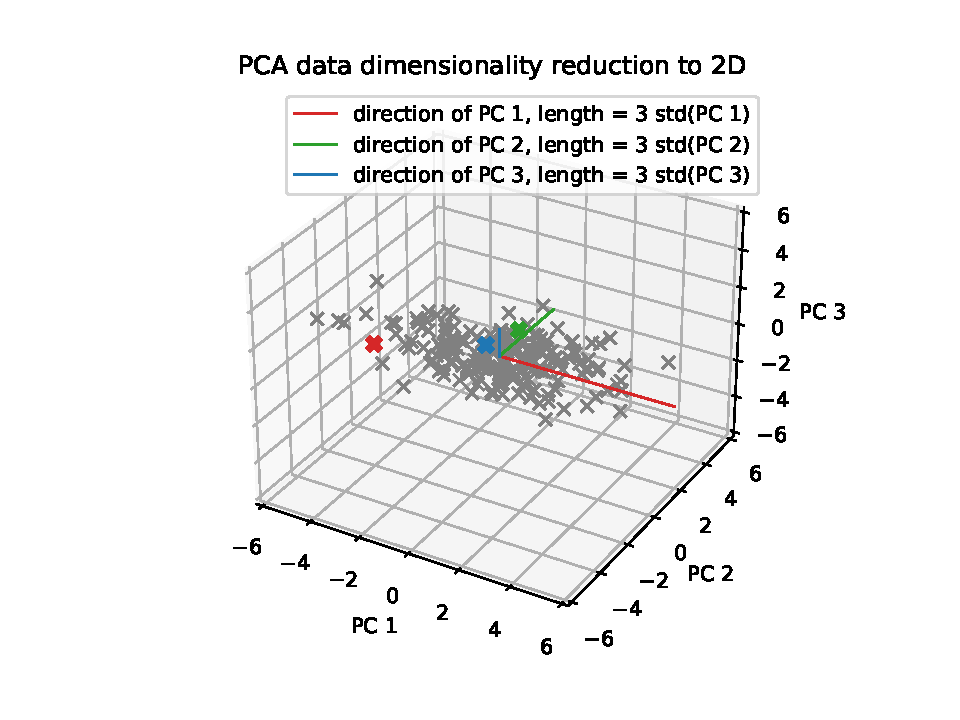
\includegraphics[width=\textwidth]{pca_3d_dim_red.pdf}
\end{minipage}
\end{frame}




\section{Section III: Train Models}
\begin{frame}[t]{Ex 09: Bias-Variance Trade Off}
no slides so far
\end{frame}


\begin{frame}[t]{Ex 10: Gradient Descent}
no slides so far
\end{frame}


\end{comment}


\section{Section IV: Model Architectures}
\begin{frame}[t]{Output Layer for Regression Model}

$\cdot$ Output layer exhibits $l=1 \dots L$ perceptrons

$\cdot$ Activation function $\sigma(\cdot)$ for $l\text{-th}$ perceptron: \underline{linear}

$$\sigma(z_l) = z_l$$

$\cdot$ Derivative

$$\frac{\partial \sigma(z_l)}{\partial z_l} = 1$$

\end{frame}



\begin{frame}[t]{Output Layer for Binary Classification Model}

$\cdot$ Output layer exhibits two perceptrons with shared input weights, hence acting on same $z$

$\cdot$ Activation functions $\sigma(\cdot)_{1,2}$ for the two perceptrons: \underline{sigmoid} / complementary sigmoid

$$\sigma_1(z) = \frac{1}{1+\e^{-z}} = \frac{\e^{z}}{\e^{z}+1} \qquad\qquad \sigma_2(z) = 1-\sigma_1(z) = \frac{1}{1 + \e^{z}} = \frac{\e^{-z}}{\e^{-z}+1}$$

\begin{center}
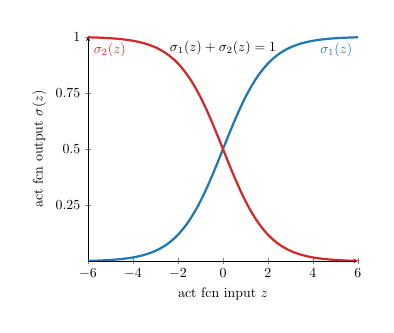
\begin{tikzpicture}[scale=0.5]
\begin{axis}[
    axis lines=left,
    xmin = -6,
    xmax = 6,
    ymax = 1,
    ytick = {0,0.25,0.5,0.75,1},
    ylabel={act fcn output $\sigma(z)$},
    xlabel={act fcn input $z$},
    ]
    \addplot [domain=-6:6,samples=128, ultra thick, C0] {exp(x)/(exp(x)+1)}
        node [pos=1, below left] {$\sigma_1(z)$};
    \addplot [domain=-6:6,samples=128, ultra thick, C3] {exp(-x)/(exp(-x)+1)}
        node [pos=0, below right] {$\sigma_2(z)$};
    \node at (0,0.95) {$\sigma_1(z)+\sigma_2(z)=1$};
\end{axis}
\end{tikzpicture}
\end{center}

$\cdot$ Derivatives

$$\frac{\partial \sigma_1(z)}{\partial z} = \frac{\e^{z}}{(\e^{z}+1)^2} = \sigma_1(z) \cdot (1-\sigma_1(z)) \qquad\qquad \frac{\partial \sigma_2(z)}{\partial z} = - \frac{\partial \sigma_1(z)}{\partial z} $$

\end{frame}



\begin{frame}[t]{Output Layer for Binary Classification Model}

$\cdot$ Output layer exhibits a single perceptron

$\cdot$ Activation function $\sigma(\cdot)$ for this single output perceptron: \underline{sigmoid}

$$\sigma(z) = \frac{1}{1+\e^{-z}} = \frac{\e^{z}}{\e^{z}+1}$$

\begin{center}
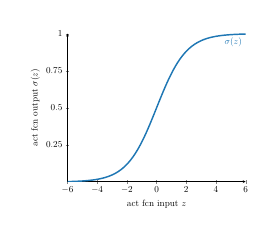
\begin{tikzpicture}[scale=0.33]
\begin{axis}[
    axis lines=left,
    xmin = -6,
    xmax = 6,
    ymax = 1,
    ytick = {0,0.25,0.5,0.75,1},
    xlabel={act fcn input $z$},
    ylabel={act fcn output $\sigma(z)$},
    ]
    \addplot [domain=-6:6,samples=128, ultra thick, C0] {exp(x)/(exp(x)+1)}
        node [pos=1, below left] {$\sigma(z)$};
\end{axis}
\end{tikzpicture}
\end{center}

$\cdot$ Derivative

$$\frac{\partial \sigma(z)}{\partial z} = \frac{\e^{z}}{(\e^{z}+1)^2} = \sigma(z) \cdot (1-\sigma(z))$$

$\cdot$ Well known as \underline{binary logistic regression} for a model with the output layer only, but no other (non-linear, hidden) layers $\rightarrow$ cf. textbooks on generalized linear models (GLMs)

\end{frame}



\begin{frame}[t]{Output Layer for Multiclass Classification Model}

$\cdot$ Output layer exhibits $l=1 \dots L$ perceptrons for $L$ classes

$\cdot$ Activation function $\sigma(\cdot)$ for $l\text{-th}$ perceptron: \underline{softmax}

$$\sigma(z_l) = \frac{\e^{z_l}}{\sum\limits_{l'=1}^{L} \e^{z_{l'}}} \qquad \text{hence, }\sum\limits_{l=1}^{L} \sigma(z_l) = 1$$

$\cdot$ Derivatives to set up the Jacobian matrix

$$\frac{\partial \sigma(z_l)}{\partial z_l} = \frac{\e^{z_l}}{\left(\sum\limits_{l'=1}^{L} \e^{z_{l'}}\right)^2} \cdot \left(\sum\limits_{l'=1, l' \neq l}^{L} \e^{z_{l'}}\right)=
\frac{\e^{z_l}}{\left(\sum\limits_{l'=1}^{L} \e^{z_{l'}}\right)} \cdot
\frac{\left(\sum\limits_{l'=1, l' \neq l}^{L} \e^{z_{l'}}\right)}{\left(\sum\limits_{l'=1}^{L} \e^{z_{l'}}\right)}=
\sigma(z_l) \cdot(1-\sigma(z_l))
$$

$$\frac{\partial \sigma(z_l)}{\partial z_j} = - \sigma(z_l) \cdot \sigma(z_j)\qquad l \neq j$$

$\cdot$ Well known as \underline{multinomial logistic regression} for a model with the output layer only, but no other (non-linear, hidden) layers $\rightarrow$ cf. textbooks on generalized linear models (GLMs)


\end{frame}


\begin{frame}[t]{Typical Loss Functions Used In Numerical Optimization}

Loss is about comparing train/val/test data $\bm{y}, y$ against model prediction data $\hat{\bm{y}}, \hat{y}$

$\cdot$ \textcolor{C0}{Regression} with least squares for predicted data sample $\hat{y}_l = \sigma_\text{\textcolor{C0}{linear}}(z_l)$; $\bm{y}\in\mathbb{R}, \hat{\bm{y}}\in\mathbb{R}$

$$\mathcal{L}(\bm{y}, \hat{\bm{y}}) = \sum\limits_{l=1}^{L} (y_l-\hat{y}_l)^2$$

$\cdot$ \textcolor{C0}{Binary classification} for predicted data sample $\hat{y} = \sigma_\text{\textcolor{C0}{sigmoid}}(z)$; $y \in \{0,1\}, 0 \leq \hat{y} \leq 1$

$$\mathcal{L}(y, \hat{y}) = -\left[y \log_\e(\hat{y}) + (1-y)\log_\e(1-\hat{y})\right]$$

$\cdot$ \textcolor{C0}{Multiclass classification} for predicted data sample $\hat{y}_l = \sigma_\text{\textcolor{C0}{softmax}}(z_l)$; $y_l \in \{0,1\}, 0 \leq \hat{y}_l \leq 1$

note: $L$ mutually exclusive classes

$$\mathcal{L}(\bm{y}, \hat{\bm{y}}) = - \left[\sum\limits_{l=1}^{L} y_l \log_\e(\hat{y}_l)\right]$$

Empirical risk for $N$ data samples
$$\mathcal{R} = \frac{1}{N} \sum\limits_{n=1}^{N} \mathcal{L}(\bm{y}_n, \hat{\bm{y}}_n)$$


\end{frame}




\begin{frame}[t]{Ex11: Linear Model for XOR (...is not working)}

XOR mapping well known as
\begin{align*}
\bm{X} =
\begin{bmatrix}
0 & 0\\
0 & 1\\
1 & 0\\
1 & 1
\end{bmatrix}\qquad
\bm{y} =
\begin{bmatrix}
0\\
1\\
1\\
0
\end{bmatrix}
\end{align*}
Simple linear model with least squares error solution
$$\bm{X} \bm{\theta} = \bm{y} \rightarrow \hat{\bm{\theta}} = (\bm{X}^\mathrm{T} \bm{X})^{-1} \bm{X}^\mathrm{T} \bm{y}
=
\frac{1}{3}\cdot
\begin{bmatrix}
1\\
1
\end{bmatrix}
$$
is not a convincing solution, because the model prediction
\begin{align*}
\bm{X} \hat{\bm{\theta}} =
\frac{1}{3}
\begin{bmatrix}
0\\
0\\
1\\
1
\end{bmatrix}
+
\frac{1}{3}
\begin{bmatrix}
0\\
1\\
0\\
1
\end{bmatrix}
=
\frac{1}{3}\cdot
\begin{bmatrix}
0\\
1\\
1\\
2
\end{bmatrix}
=\hat{\bm{y}}
\end{align*}
does not yield XOR. This is because $\bm{y}$ is not in the column space of $\bm{X}$ and
the resulting column space solution $\hat{\bm{y}}$
is useless for the intended application

\end{frame}






\begin{frame}[t]{Try Another Linear Model for XOR (...is not working either)}

Feature matrix with additional typical \underline{intercept} represented by the \underline{first column} in $\bm{X}$
\begin{align*}
\bm{X} =
\begin{bmatrix}
1 & 0 & 0\\
1 & 0 & 1\\
1 & 1 & 0\\
1 & 1 & 1
\end{bmatrix}\qquad
\bm{y} =
\begin{bmatrix}
0\\
1\\
1\\
0
\end{bmatrix}
\end{align*}
...but XOR-result $\bm{y}$ is again not in the column space of $\bm{X}$


Least squares error solution
$$\hat{\bm{\theta}} = (\bm{X}^\mathrm{T} \bm{X})^{-1} \bm{X}^\mathrm{T} \bm{y}
=
\frac{1}{2}\cdot
\begin{bmatrix}
1\\
0\\
0
\end{bmatrix}
$$
Prediction
\begin{align*}
\bm{X} \hat{\bm{\theta}} =
\frac{1}{2}
\begin{bmatrix}
1\\
1\\
1\\
1
\end{bmatrix}
+
0
\begin{bmatrix}
0\\
0\\
1\\
1
\end{bmatrix}
+
0
\begin{bmatrix}
0\\
1\\
0\\
1
\end{bmatrix}
=
\frac{1}{2}\cdot
\begin{bmatrix}
1\\
1\\
1\\
1
\end{bmatrix}
=\hat{\bm{y}} \neq \bm{y}
\end{align*}
\end{frame}







\begin{frame}[t]{Non-Linear Model for XOR}
%
\begin{center}
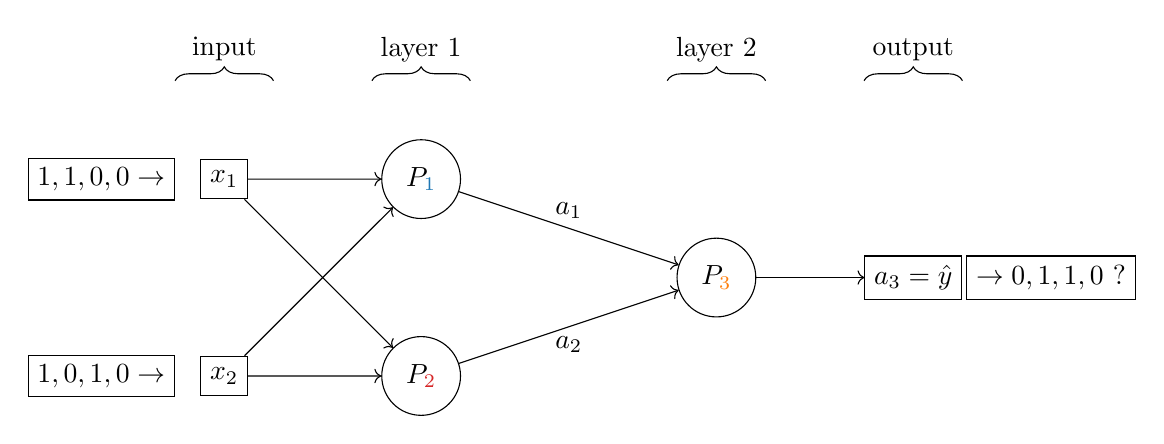
\begin{tikzpicture}[scale=1.25]
\tikzstyle{iol}=[draw,shape=rectangle,minimum size=0.5cm]
\tikzstyle{hl}=[draw,shape=circle,minimum size=1cm]

\node[iol](x0d) at (-1.25,+1){$1,1,0,0\rightarrow$};
\node[iol](x1d) at (-1.25,-1){$1,0,1,0\rightarrow$};
%
\node[iol](x0) at (0,+1){$x_1$};
\node[iol](x1) at (0,-1){$x_2$};
\node[hl](l1p1) at (2,+1){$P_{\textcolor{C0}{1}}$};
\node[hl](l1p2) at (2,-1){$P_{\textcolor{C3}{2}}$};
\node[hl](l2p1) at (5,0){$P_{\textcolor{C1}{3}}$};
\node[iol](y) at (7,0){$a_3=\hat{y}$};
%
\node[iol](yd) at (8.4,+0){$\rightarrow 0,1,1,0 \,\,?$};
%
\draw[->] (x0) -- (l1p1);
\draw[->] (x0) -- (l1p2);
\draw[->] (x1) -- (l1p1);
\draw[->] (x1) -- (l1p2);
\draw[->] (l1p1) -- (l2p1)node[midway, above]{$a_1$};
\draw[->] (l1p2) -- (l2p1)node[midway, below]{$a_2$};
\draw[->] (l2p1) -- (y);
%
\draw [decorate,decoration={brace,amplitude=5pt}] (-0.5,2) -- (0.5,2) node [black,midway,yshift=0.4cm]{input};
\draw [decorate,decoration={brace,amplitude=5pt}] (1.5,2) -- (2.5,2) node [black,midway,yshift=0.4cm]{layer 1};
\draw [decorate,decoration={brace,amplitude=5pt}] (4.5,2) -- (5.5,2) node [black,midway,yshift=0.4cm]{layer 2};
\draw [decorate,decoration={brace,amplitude=5pt}] (6.5,2) -- (7.5,2) node [black,midway,yshift=0.4cm]{output};
\end{tikzpicture}
\end{center}
%
\end{frame}





\begin{frame}[t]{Non-Linear Model for XOR}
%
\begin{center}
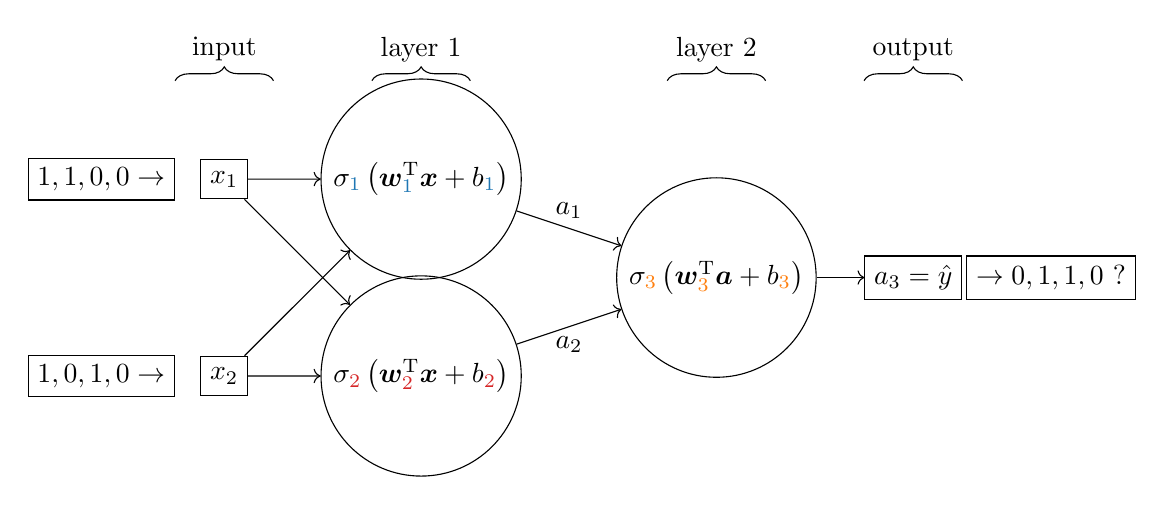
\begin{tikzpicture}[scale=1.25]
\tikzstyle{iol}=[draw,shape=rectangle,minimum size=0.5cm]
\tikzstyle{hl}=[draw,shape=circle,minimum size=2cm]

\node[iol](x0d) at (-1.25,+1){$1,1,0,0\rightarrow$};
\node[iol](x1d) at (-1.25,-1){$1,0,1,0\rightarrow$};
%
\node[iol](x0) at (0,+1){$x_1$};
\node[iol](x1) at (0,-1){$x_2$};
\node[hl](l1p1) at (2,+1){$\sigma_{\textcolor{C0}{1}}\left({\bm{w}_{\textcolor{C0}{1}}^\mathrm{T}\bm{x} + b_{\textcolor{C0}{1}}}\right)$};
\node[hl](l1p2) at (2,-1){$\sigma_{\textcolor{C3}{2}}\left({\bm{w}_{\textcolor{C3}{2}}^\mathrm{T}\bm{x} + b_{\textcolor{C3}{2}}}\right)$};
\node[hl](l2p1) at (5,0){$\sigma_{\textcolor{C1}{3}}\left({\bm{w}_{\textcolor{C1}{3}}^\mathrm{T}\bm{a} + b_{\textcolor{C1}{3}}}\right)$};
\node[iol](y) at (7,0){$a_3=\hat{y}$};
%
\node[iol](yd) at (8.4,+0){$\rightarrow 0,1,1,0 \,\,?$};
%
\draw[->] (x0) -- (l1p1);
\draw[->] (x0) -- (l1p2);
\draw[->] (x1) -- (l1p1);
\draw[->] (x1) -- (l1p2);
\draw[->] (l1p1) -- (l2p1)node[midway, above]{$a_1$};
\draw[->] (l1p2) -- (l2p1)node[midway, below]{$a_2$};
\draw[->] (l2p1) -- (y);
%
\draw [decorate,decoration={brace,amplitude=5pt}] (-0.5,2) -- (0.5,2) node [black,midway,yshift=0.4cm]{input};
\draw [decorate,decoration={brace,amplitude=5pt}] (1.5,2) -- (2.5,2) node [black,midway,yshift=0.4cm]{layer 1};
\draw [decorate,decoration={brace,amplitude=5pt}] (4.5,2) -- (5.5,2) node [black,midway,yshift=0.4cm]{layer 2};
\draw [decorate,decoration={brace,amplitude=5pt}] (6.5,2) -- (7.5,2) node [black,midway,yshift=0.4cm]{output};
\end{tikzpicture}
\end{center}
%
\end{frame}




\begin{frame}[t]{Non-Linear Model for XOR}

$\cdot$ weight matrix and bias vector to represent perceptron \textcolor{C0}{1} and \textcolor{C3}{2}
$$
\bm{W}_\text{layer 1} =
\begin{bmatrix}
w_{1\textcolor{C0}{1}} & w_{1\textcolor{C3}{2}}\\
w_{2\textcolor{C0}{1}} & w_{2\textcolor{C3}{2}}
\end{bmatrix}
\qquad
\bm{b}_\text{layer 1}
=
\begin{bmatrix}
b_{\textcolor{C0}{1}}\\
b_{\textcolor{C3}{2}}
\end{bmatrix}
$$

$\cdot$ weight vector and bias scalar to represent perceptron \textcolor{C1}{3}
$$
\bm{W}_\text{layer 2} =
\begin{bmatrix}
w_{1\textcolor{C1}{3}}\\
w_{2\textcolor{C1}{3}}
\end{bmatrix}
\qquad
\bm{b}_\text{layer 2}=[b_{\textcolor{C1}{3}}]
$$

$\cdot$ model prediction for $\bm{x} = [x_1, x_2]^\mathrm{T}$

\begin{align*}
\bm{a} =
\begin{bmatrix}
a_1\\
a_2
\end{bmatrix}=
\mathrm{max}\left\{\bm{0},\,\,\,\bm{W}_\text{layer 1}^\mathrm{T} \bm{x} + \bm{b}_\text{layer 1}\right\}
&\qquad\text{with ReLU activation}\,\,\,
\sigma_{1,2}(\bm{z}) = \mathrm{max}\left\{\bm{0}, \bm{z}\right\}
\\
a_3 = \hat{y} = \bm{W}_\text{layer 2}^\mathrm{T} \bm{a} + \bm{b}_\text{layer 2}
&\qquad\text{with linear activation}\,\,\,
\sigma_{3}(\bm{z}) = \bm{z}
\end{align*}
$\cdot$ model prediction in one line
\begin{align*}
a_3 = \hat{y} = \bm{W}_\text{layer 2}^\mathrm{T}
\mathrm{max}\left\{\bm{0},\,\,\,\bm{W}_\text{layer 1}^\mathrm{T} \bm{x} + \bm{b}_\text{layer 1}\right\}
+ \bm{b}_\text{layer 2}
\end{align*}


\end{frame}



\begin{frame}[t]{Non-Linear Model for XOR}

$\cdot$ solution known from book Goodfellow et al. (2016): Deep Learning. MIT Press, Ch. 6.1

$\cdot$ weight matrix and bias vector to represent perceptron \textcolor{C0}{1} and \textcolor{C3}{2}
$$
\bm{W}_\text{layer 1} =
\begin{bmatrix}
w_{1\textcolor{C0}{1}}=1 & w_{1\textcolor{C3}{2}}=1\\
w_{2\textcolor{C0}{1}}=1 & w_{2\textcolor{C3}{2}}=1
\end{bmatrix}
\qquad
\bm{b}_\text{layer 1}
=
\begin{bmatrix}
b_{\textcolor{C0}{1}} = 0\\
b_{\textcolor{C3}{2}} = -1
\end{bmatrix}
$$

$\cdot$ weight vector and bias scalar to represent perceptron \textcolor{C1}{3}
$$
\bm{W}_\text{layer 2} =
\begin{bmatrix}
w_{1\textcolor{C1}{3}} = 1\\
w_{2\textcolor{C1}{3}} = -2
\end{bmatrix}
\qquad
\bm{b}_\text{layer 2}=[b_{\textcolor{C1}{3}} = 0]
$$

$\cdot$ predict for $\bm{x} = [1, 0]^\mathrm{T}$ where true XOR-result is $y = 1$

\begin{align*}
\bm{a} =
\begin{bmatrix}
1\\
0
\end{bmatrix}=
\mathrm{max}\left\{
\begin{bmatrix}
0\\
0
\end{bmatrix}
,\,\,\,
\begin{bmatrix}
1&1\\
1&1
\end{bmatrix}
^\mathrm{T}
\begin{bmatrix}
1\\
0
\end{bmatrix}
+
\begin{bmatrix}
0\\
-1
\end{bmatrix}
\right\}
&\qquad\text{with ReLU activation}\,\,\,
\sigma_{1,2}(\bm{z}) = \mathrm{max}\left\{\bm{0}, \bm{z}\right\}
\\
a_3 = \hat{y} = \begin{bmatrix}
1\\
-2
\end{bmatrix}^\mathrm{T}
\begin{bmatrix}
1\\
0
\end{bmatrix}
+ 0 = 1
&\qquad\text{with linear activation}\,\,\,
\sigma_{3}(\bm{z}) = (\bm{z})
\end{align*}

$\cdot$ predict the other three cases...to make sure everything is fine

\end{frame}

\begin{frame}[t]{Non-Linear Model for XOR}
The model prediction output $\hat{y}$ is a function of the input data sample and the 9 model parameters (6 weights, 3 bias terms)
$$
\hat{y}\left(\bm{x},\bm{W}_\text{layer 1}, \bm{b}_\text{layer 1}
\bm{W}_\text{layer 2}, \bm{b}_\text{layer 2}\right)
=
\bm{W}_\text{layer 2}^\mathrm{T}
\mathrm{max}\left\{\bm{0},\,\,\,\bm{W}_\text{layer 1}^\mathrm{T} \bm{x} + \bm{b}_\text{layer 1}\right\}
+ \bm{b}_\text{layer 2}
$$
Hence, definition of an appropriate loss function is required
$$
\mathcal{L}\left(y,\quad\hat{y}\left(\bm{x}_n, \bm{W}_\text{layer 1}, \bm{b}_\text{layer 1}
\bm{W}_\text{layer 2}, \bm{b}_\text{layer 2}\right)\right)
$$

The above solution was found with the mean squared error (MSE) empirical risk function
$$\mathcal{R} = \frac{1}{4}\sum_{n=1}^4 \mathcal{L}_n(y, \hat{y}) = \frac{1}{4}\sum_{n=1}^4 (y_n-\hat{y}_n)^2 = \frac{1}{4}\lVert\bm{y} - \hat{\bm{y}}\rVert_2^2$$
to be minimized by $\operatorname*{argmin}_{\bm{W}_\text{layer 1}, \bm{b}_\text{layer 1}
\bm{W}_\text{layer 2}, \bm{b}_\text{layer 2}} \mathcal{R}$.

Why is it tricky to solve this MSE risk numerically by gradient descent?

What could be another model architecture and/or loss function for the given problem?

% https://medium.com/@lucaspereira0612/solving-xor-with-a-single-perceptron-34539f395182
% https://towardsdatascience.com/perceptrons-logical-functions-and-the-xor-problem-37ca5025790a

%9 model parameters (7 non-zero model parameters) vs. 8+4 data samples

\end{frame}





\begin{frame}{Modeling Non-Linearity with Bias and Activation Function}
%
\begin{flushright}
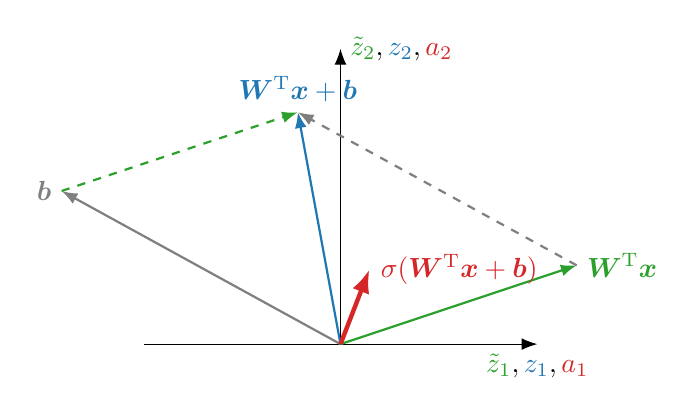
\begin{tikzpicture}
  %sig_out = [exp(-1), 0.95]
  %sig_in = log(sig_out./(1-sig_out))
  %wx = [3 1]
  %bias = sig_in - wx
  %wx + bias
  %sigmoid(wx + bias) == sig_out
  %function zo = sigmoid(zi)
  %    zo = exp(zi) ./ (1+exp(zi));
  %end
\coordinate (wx) at (3,1);
\coordinate (bias) at (-3.54132485461292, 1.94443897916644);
\coordinate (wxbias) at ($(wx)+(bias)$); % must match the point:
%\coordinate (sigmoid_in) at (-0.541324854612918,2.94443897916644);
\coordinate (sigmoid_out) at (0.367879441171442,0.95);
%
\draw[-{Latex[length=2mm]}] (-2.5,0) -- (2.5,0)node[below]{$\textcolor{C2}{\tilde{z}_1}, \textcolor{C0}{z_1}, \textcolor{C3}{a_1}$};
\draw[-{Latex[length=2mm]}] (0,0) -- (0,3.75)node[right]{$\textcolor{C2}{\tilde{z}_2}, \textcolor{C0}{z_2}, \textcolor{C3}{a_2}$};
%
\draw[-{Latex[length=2mm]}, thick, C2] (0,0) -- (wx)node[below, right]{$\bm{W}^\mathrm{T} \bm{x}$};
\draw[-{Latex[length=2mm]}, thick, dashed, C7] (wx) -- (wxbias);
\draw[-{Latex[length=2mm]}, thick, C7] (0,0) -- (bias)node[above, left]{$\bm{b}$};
\draw[-{Latex[length=2mm]}, thick, dashed, C2] (bias) -- (wxbias);
\draw[-{Latex[length=2mm]}, thick, C0] (0,0) -- (wxbias)node[left, above]{$\bm{W}^\mathrm{T} \bm{x}+\bm{b}$};
\draw[-{Latex[length=3mm]}, ultra thick, C3] (0,0) -- (sigmoid_out)node[above, right]{$\sigma(\bm{W}^\mathrm{T} \bm{x}+\bm{b})$};
\end{tikzpicture}
\end{flushright}
\end{frame}


\begin{frame}[t]{Ex12: Binary Classification / Binary Logistic Regression}

\begin{center}
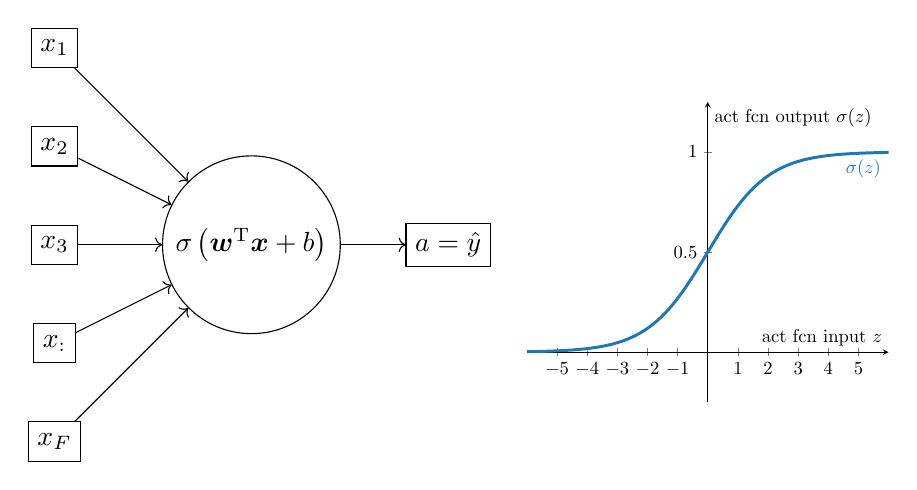
\begin{tikzpicture} %[scale=1.25]
%
\begin{scope}[scale=1.25]
\tikzstyle{iol}=[draw,shape=rectangle,minimum size=0.5cm]
\tikzstyle{hl}=[draw,shape=circle,minimum size=2cm]
%
\node[iol](x1) at (0,+2){$x_1$};
\node[iol](x2) at (0,+1){$x_2$};
\node[iol](x3) at (0,0){$x_3$};
\node[iol](xf) at (0,-1){$x_:$};
\node[iol](xF) at (0,-2){$x_F$};

\node[hl](l1p1) at (2,0){$\sigma\left(\bm{w}^\mathrm{T}\bm{x} + b\right)$};
\node[iol](y) at (4,0){$a=\hat{y}$};
%
\draw[->] (x1) -- (l1p1);
\draw[->] (x2) -- (l1p1);
\draw[->] (x3) -- (l1p1);
\draw[->] (xf) -- (l1p1);
\draw[->] (xF) -- (l1p1);
\draw[->] (l1p1) -- (y);
%
\end{scope}
%
\begin{scope}[shift={(6,-2)}, scale=0.67]
\begin{axis}[
    axis lines=middle,
    xmin = -6,
    xmax = 6,
    ymin = -0.25,
    ymax = 1.25,
    xtick = {-5,...,5},
    ytick = {0,0.5,1},
    xlabel={act fcn input $z$},
    ylabel={act fcn output $\sigma(z)$},
    ]
    \addplot [domain=-6:6,samples=128, ultra thick, C0] {exp(x)/(exp(x)+1)}
        node [pos=1, below left] {$\sigma(z)$};
\end{axis}
\end{scope}
\end{tikzpicture}
\end{center}

$\cdot$ Activation function $\sigma(\cdot)$ for this single output perceptron: \underline{sigmoid}

$$\hat{y} = \sigma(z) = \frac{1}{1+\e^{-z}} = \frac{\e^{z}}{\e^{z}+1}\qquad\qquad
\frac{\partial \sigma(z)}{\partial z} = \frac{\e^{z}}{(\e^{z}+1)^2} = \sigma(z) \cdot (1-\sigma(z))
$$

\end{frame}


\begin{frame}[t]{Loss Function For Binary Logistic Regression / Binary Cross Entropy}

$\cdot$ Loss function for $y\in\{0,1\}$ and predicted output $\textcolor{C0}{\hat{y}} \in\mathbb{R},\,\,\,0 \leq \textcolor{C0}{\hat{y}} \leq 1$ / empirical risk

$$\mathcal{L}_n(y, \textcolor{C0}{\hat{y}}) = -\left[y_n \log_\e(\textcolor{C0}{\hat{y}_n}) + (1-y_n) \log_\e(1-\textcolor{C0}{\hat{y}_n})\right]
\qquad\quad
\mathcal{R} = \frac{1}{N} \sum\limits_{n=1}^N \mathcal{L}_n(y, \textcolor{C0}{\hat{y}})
$$


\begin{center}
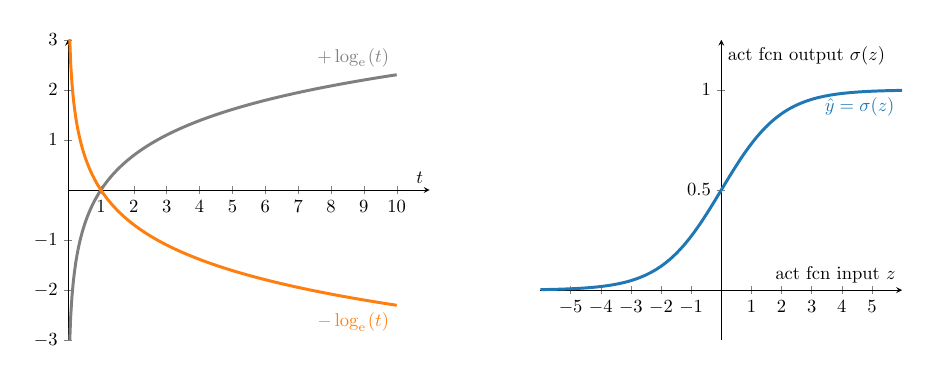
\begin{tikzpicture} %[scale=1.25]
%
\begin{scope}[shift={(0,0)}, scale=0.67]
\begin{axis}[
    axis lines=middle,
    xmin = 0,
    xmax = 11,
    ymin = -3,
    ymax = 3,
    xtick = {0,...,10},
    ytick = {-3,...,3},
    xlabel={$t$},
    ylabel={},
    ]
    \addplot [domain=0:10,samples=256, ultra thick, C7] {ln(x))}
        node [pos=1, above left] {$+\log_\e(t)$};
    \addplot [domain=0:10,samples=256, ultra thick, C1] {-ln(x))}
            node [pos=1, below left] {$-\log_\e(t)$};
\end{axis}
\end{scope}
%
\begin{scope}[shift={(6,0)}, scale=0.67]
\begin{axis}[
    axis lines=middle,
    xmin = -6,
    xmax = 6,
    ymin = -0.25,
    ymax = 1.25,
    xtick = {-5,...,5},
    ytick = {0,0.5,1},
    xlabel={act fcn input $z$},
    ylabel={act fcn output $\sigma(z)$},
    ]
    \addplot [domain=-6:6,samples=128, ultra thick, C0] {exp(x)/(exp(x)+1)}
        node [pos=1, below left] {$\hat{y} = \sigma(z)$};
\end{axis}
\end{scope}
\end{tikzpicture}
\end{center}

\begin{minipage}[t]{0.49\textwidth}
$\mathcal{L}_n(y=0, \hat{y})
=
\textcolor{C1}{-}\left[\textcolor{C1}{\log_\e}(1-\textcolor{C0}{\hat{y}_n})\right]
$

$\textcolor{C0}{\hat{y}_n} \approx 0 \rightarrow \,?$

$\textcolor{C0}{\hat{y}_n} \approx 1 \rightarrow \,?$
\end{minipage}
\begin{minipage}[t]{0.49\textwidth}
$\mathcal{L}_n(y=1, \hat{y})
=
\textcolor{C1}{-}\left[\textcolor{C1}{\log_\e}(\textcolor{C0}{\hat{y}_n})\right]
$

$\textcolor{C0}{\hat{y}_n} \approx 0 \rightarrow \,?$

$\textcolor{C0}{\hat{y}_n} \approx 1 \rightarrow \,?$
\end{minipage}

\end{frame}





\begin{frame}{Model Training / Solve Minimization Problem by Gradient Descent}

\begin{align*}
\operatorname*{argmin}_{\bm{w}, b} \mathcal{R} =
&\operatorname*{argmin}_{\bm{w}, b} \frac{1}{N} \sum\limits_{n=1}^N -\left[y_n \log_\e(\textcolor{C0}{\hat{y}_n}) + (1-y_n) \log_\e(1-\textcolor{C0}{\hat{y}_n})\right]=\\
&\operatorname*{argmin}_{\bm{w}, b} \frac{1}{N} \sum\limits_{n=1}^N -\left[y_n \log_\e(\textcolor{C0}{\sigma\left(\bm{w}^\mathrm{T}\bm{x}_n + b\right)}) + (1-y_n) \log_\e(1-\textcolor{C0}{\sigma\left(\bm{w}^\mathrm{T}\bm{x}_n + b\right)})\right]
\end{align*}

%$\cdot$ solve by (full-batch $N$ data samples) gradient descent (GD):

$\cdot$ randomly init weights $\bm{w}, b$ to be used as actual state

1. prediction $\textcolor{C0}{\sigma\left(\bm{w}^\mathrm{T}\bm{x}_n + b\right)}$ (and store intermediate results for back prop)

2. calc empiral risk $\mathcal{R} = J(\bm{w}, b)$ (and store intermediate results for back prop)

3. evaluate gradient
$$\left[
\frac{\partial J}{\partial w_1}\bigg|_{w_1=w_{1,\text{act}}},
\dots,
\frac{\partial J}{\partial w_F}\bigg|_{w_F=w_{F,\text{act}}},
\frac{\partial J}{\partial b  }\bigg|_{b  =b_{  \text{act}}}\right]^\mathrm{T}$$

4. gradient descent (GD) update rule with learning rate / step size $\gamma$
$$w_{:,\text{new act}} = w_{:,\text{act}} - \gamma \frac{\partial J}{\partial w_:}\bigg|_{w_:=w_{:,\text{act}}}
\qquad
b_{\text{new act}} = b_{\text{act}} - \gamma \frac{\partial J}{\partial b}\bigg|_{b=b_{\text{act}}}$$

$\cdot$ repeat steps 1 to 4 until a given stop criterion is fullfilled
\end{frame}

\begin{frame}[t]{First Derivative of Loss / Empirical Risk}

Loss / empirical risk
$$\mathcal{L}_n(y, \textcolor{C0}{\hat{y}}) = -\left[y_n \log_\e(\textcolor{C0}{\hat{y}_n}) + (1-y_n) \log_\e(1-\textcolor{C0}{\hat{y}_n})\right]
\qquad\quad
J(\bm{w},b) = \frac{1}{N} \sum\limits_{n=1}^N \mathcal{L}_n(y, \textcolor{C0}{\hat{y}})
$$
%
First derivative of empirical risk vs. loss
$$
\frac{\partial J(\bm{w},b)}{\partial \bm{w}\cdots\partial b} =
\frac{\partial \left(\frac{1}{N} \sum\limits_{n=1}^N \mathcal{L}_n(y, \textcolor{C0}{\hat{y}})\right)}{\partial \bm{w}\cdots\partial b}=
\frac{1}{N} \sum\limits_{n=1}^N \frac{\partial \mathcal{L}_n(y, \textcolor{C0}{\hat{y}})}{\partial \bm{w}\cdots\partial b}
$$
%
We need to analytically know these derivatives as we will use them in GD
$$
\frac{\partial \mathcal{L}_n(y, \textcolor{C0}{\hat{y}})}{\partial \bm{w}\cdots\partial b} =
-\frac{\partial
\left[y_n \log_\e(\textcolor{C0}{\sigma\left(\bm{w}^\mathrm{T}\bm{x}_n + b\right)}) + (1-y_n) \log_\e(1-\textcolor{C0}{\sigma\left(\bm{w}^\mathrm{T}\bm{x}_n + b\right)})\right]
}{\partial \bm{w}\cdots\partial b}
$$


\end{frame}



\begin{frame}[t]{First Derivative of Loss}

Recap that we use the sigmoid activation for binary classification
$$\textcolor{C0}{\hat{y}} = \sigma(z) = \frac{1}{1+\e^{-z}} = \frac{\e^{z}}{\e^{z}+1}\qquad\qquad
\frac{\partial \sigma(z)}{\partial z} = \frac{\e^{z}}{(\e^{z}+1)^2} = \sigma(z) \cdot (1-\sigma(z))
$$
%
Check for $w_1$
\begin{align*}
&z = \zeta(w_1) = \bm{w}^\mathrm{T}\bm{x} + b\\
&\textcolor{C0}{\hat{y}} = \sigma(z) = \sigma(\zeta(w_1)) = \sigma\left(\bm{w}^\mathrm{T}\bm{x} + b\right)
\end{align*}
%
$$
\frac{\partial \mathcal{L}(y, \textcolor{C0}{\hat{y}})}{\partial w_1} =
\frac{\partial \mathcal{L}}{\partial \textcolor{C0}{\hat{y}}} \cdot
\frac{\partial \textcolor{C0}{\hat{y}}}{\partial z} \cdot
\frac{\partial z}{\partial w_1}
\qquad\qquad
\frac{\partial \mathcal{L}(y, \textcolor{C0}{\hat{y}})}{\partial w_1} =
\frac{\partial \mathcal{L}}{\partial \sigma(\zeta(w_1))} \cdot
\frac{\partial \sigma(\zeta(w_1))}{\partial \zeta(w_1)} \cdot
\frac{\partial \zeta(w_1)}{\partial w_1}
$$
%
For GD we need
$$
\frac{\partial \mathcal{L}(y, \textcolor{C0}{\hat{y}})}{\partial w_1}\bigg|_{w_{1,\text{act}}} =
\frac{\partial \mathcal{L}}{\partial \textcolor{C0}{\hat{y}}}\bigg|_{\hat{y}(w_{1,\text{act}})} \cdot
\frac{\partial \textcolor{C0}{\hat{y}}}{\partial z}\bigg|_{z(w_{1,\text{act}})} \cdot
\frac{\partial z}{\partial w_1}\bigg|_{w_{1,\text{act}}}
$$
%
Hence, analytical expressions
$$
\frac{\partial \mathcal{L}}{\partial \textcolor{C0}{\hat{y}}} = -\left[\frac{y}{\textcolor{C0}{\hat{y}}}+(-1)\frac{1-y}{1-\textcolor{C0}{\hat{y}}}\right]
\qquad\qquad
\frac{\partial \textcolor{C0}{\hat{y}}}{\partial z} = \textcolor{C0}{\hat{y}} (1-\textcolor{C0}{\hat{y}})
\qquad\qquad
\frac{\partial z}{\partial w_1} = x_1
$$

\end{frame}







\begin{frame}[t]{All Partial Derivatives for Loss and Empirical Risk}

For GD we need all partial derivatives, i.e. w.r.t $w_1 \dots w_F$ and $b$
\begin{align*}
&\frac{\partial \mathcal{L}(y, \textcolor{C0}{\hat{y}})}{\partial w_:}\bigg|_{w_{:,\text{act}}} =
\frac{\partial \mathcal{L}}{\partial \textcolor{C0}{\hat{y}}}\bigg|_{\hat{y}(w_{:,\text{act}})} \cdot
\frac{\partial \textcolor{C0}{\hat{y}}}{\partial z}\bigg|_{z(w_{:,\text{act}})} \cdot
\frac{\partial z}{\partial w_:}\bigg|_{w_{:,\text{act}}}\\
&\frac{\partial \mathcal{L}(y, \textcolor{C0}{\hat{y}})}{\partial b}\bigg|_{b_{\text{act}}} =
\frac{\partial \mathcal{L}}{\partial \textcolor{C0}{\hat{y}}}\bigg|_{\hat{y}(b_{\text{act}})} \cdot
\frac{\partial \textcolor{C0}{\hat{y}}}{\partial z}\bigg|_{z(b_{\text{act}})} \cdot
\frac{\partial z}{\partial b}\bigg|_{b_{\text{act}}}
\end{align*}
%
Analytical expressions
\begin{align*}
\text{for}\quad w_: \quad &\frac{\partial \mathcal{L}}{\partial \textcolor{C0}{\hat{y}}} = -\left[\frac{y}{\textcolor{C0}{\hat{y}}}+(-1)\frac{1-y}{1-\textcolor{C0}{\hat{y}}}\right]
\qquad\qquad
\frac{\partial \textcolor{C0}{\hat{y}}}{\partial z} = \textcolor{C0}{\hat{y}} (1-\textcolor{C0}{\hat{y}})
\qquad\qquad
\frac{\partial z}{\partial w_:} = x_:\\
\text{for}\quad b \quad &\frac{\partial \mathcal{L}}{\partial \textcolor{C0}{\hat{y}}} = -\left[\frac{y}{\textcolor{C0}{\hat{y}}}+(-1)\frac{1-y}{1-\textcolor{C0}{\hat{y}}}\right]
\qquad\qquad
\frac{\partial \textcolor{C0}{\hat{y}}}{\partial z} = \textcolor{C0}{\hat{y}} (1-\textcolor{C0}{\hat{y}})
\qquad\qquad
\frac{\partial z}{\partial b} = 1
\end{align*}
%
For GD we not only use the loss of one data sample, but rather need the empirical risk
\begin{align*}
\frac{\partial J}{\partial w_:}\bigg|_{w_{:,\text{act}}} = \frac{1}{N} \sum\limits_{n=1}^N \frac{\partial \mathcal{L}_n(y, \textcolor{C0}{\hat{y}})}{\partial w_:}\bigg|_{w_{:,\text{act}}}
\qquad\qquad
\frac{\partial J}{\partial b}\bigg|_{b_{\text{act}}} = \frac{1}{N} \sum\limits_{n=1}^N\frac{\partial \mathcal{L}_n(y, \textcolor{C0}{\hat{y}})}{\partial b}\bigg|_{b_{\text{act}}}
\end{align*}

\end{frame}








\begin{frame}{Binary Classification: Numerical Example for GD Update}

\begin{minipage}[]{0.39\textwidth}
%
\begin{align*}
&\textcolor{C0}{\hat{y}} = \sigma(z) = \frac{1}{1+\e^{-z}}
\\
&\frac{\partial \mathcal{L}}{\partial \textcolor{C0}{\hat{y}}} = -\left[\frac{y}{\textcolor{C0}{\hat{y}}}+(-1)\frac{1-y}{1-\textcolor{C0}{\hat{y}}}\right]
\\
&\frac{\partial \textcolor{C0}{\hat{y}}}{\partial z} = \textcolor{C0}{\hat{y}} (1-\textcolor{C0}{\hat{y}})
\\
&\frac{\partial z}{\partial w_:} = x_:\qquad \frac{\partial z}{\partial b} = 1
\end{align*}
%
actual state:
\begin{align*}
&\bm{x} =
\begin{bmatrix}
x_1\\x_2\\x_3
\end{bmatrix}
=
\begin{bmatrix}
1\\2\\3
\end{bmatrix}
\quad
y=0\\
&\bm{w}_\text{act} =
\begin{bmatrix}
w_1\\w_2\\w_3
\end{bmatrix}
=
\begin{bmatrix}
1\\\frac{1}{2}\\\frac{1}{3}
\end{bmatrix}
\quad
b_\text{act}=1
\end{align*}
%
\end{minipage}
%
\begin{minipage}[t]{0.59\textwidth}
%
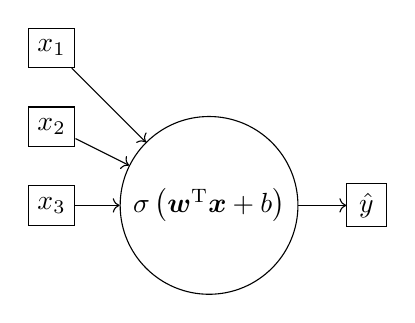
\begin{tikzpicture}[scale=1]
%
\tikzstyle{iol}=[draw,shape=rectangle,minimum size=0.5cm]
\tikzstyle{hl}=[draw,shape=circle,minimum size=2cm]
%
\node[iol](x1) at (0,+2){$x_1$};
\node[iol](x2) at (0,+1){$x_2$};
\node[iol](x3) at (0,0){$x_3$};
%
\node[hl](l1p1) at (2,0){$\sigma\left(\bm{w}^\mathrm{T}\bm{x} + b\right)$};
\node[iol](y) at (4,0){$\hat{y}$};
%
\draw[->] (x1) -- (l1p1);
\draw[->] (x2) -- (l1p1);
\draw[->] (x3) -- (l1p1);
\draw[->] (l1p1) -- (y);
\end{tikzpicture}
%

for new state / for GD update: ?
%
\pause
% clear all; clc; format long g
% % actual state
% x = [1; 2; 3];      y = 0;
% w = [1/1;1/2; 1/3]; b = 1;
% % predict / forward prop
% z = w.'*x + b; yh = 1 / (1+exp(-z));
% % partial derivatives
% dLdyh = - y/yh + (1-y)/(1-yh);
% dyhdz = yh * (1-yh);
% dzdw1 = x(1);
% dzdw2 = x(2);
% dzdw3 = x(3);
% dzdb = 1;
% % chain rule / back prop
% dLdw1 = dLdyh * dyhdz * dzdw1;
% dLdw2 = dLdyh * dyhdz * dzdw2;
% dLdw3 = dLdyh * dyhdz * dzdw3;
% dLdb = dLdyh * dyhdz * dzdb;
% % round to meaningful format for slides
% prec = 7;
% round(dLdyh,prec)
% round(dyhdz,prec)
% round(dLdw1,prec)
% round(dLdw2,prec)
% round(dLdw3,prec)
% round(dLdb,prec)
\begin{align*}
&\frac{\partial \mathcal{L}}{\partial \textcolor{C0}{\hat{y}}}\bigg|_{\hat{y}(w_{:,\text{act}}, b_{\text{act}})} = 55.59815\quad
\frac{\partial \textcolor{C0}{\hat{y}}}{\partial z}\bigg|_{z(w_{:,\text{act}}, b_{\text{act}})}= 0.0176627\\
&\frac{\partial \mathcal{L}}{\partial w_1}\bigg|_{w_{1,\text{act}}} = 0.9820138\quad
\frac{\partial \mathcal{L}}{\partial w_2}\bigg|_{w_{2,\text{act}}} = 1.9640276\\
&\frac{\partial \mathcal{L}}{\partial w_3}\bigg|_{w_{3,\text{act}}} = 2.9460414\quad
\frac{\partial \mathcal{L}}{\partial b}\bigg|_{b_{\text{act}}} = 0.9820138
\end{align*}


\end{minipage}
%
\end{frame}




\begin{frame}{Binary Classification with Hidden Layer Model}
%
\vspace{-0.75cm}
\begin{center}
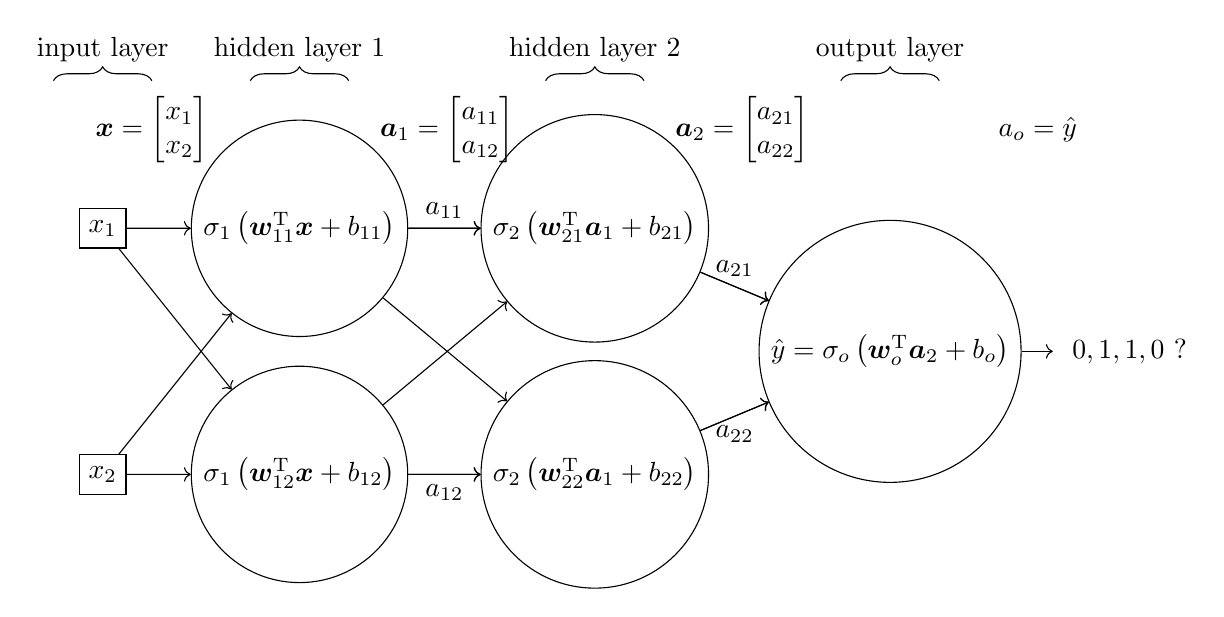
\begin{tikzpicture}[scale=1.25]
\tikzstyle{iol}=[draw,shape=rectangle,minimum size=0.5cm]
\tikzstyle{hl}=[draw,shape=circle,minimum size=2cm]
%
\node[iol](x0) at (0,+1.25){$x_1$};
\node[iol](x1) at (0,-1.25){$x_2$};
\node[hl](l1p1) at (2,+1.25){$\sigma_{1}\left(\bm{w}_{11}^\mathrm{T} \bm{x} + b_{11}\right)$};
\node[hl](l1p2) at (2,-1.25){$\sigma_{1}\left(\bm{w}_{12}^\mathrm{T} \bm{x} + b_{12}\right)$};
\node[hl](l2p1) at (5,+1.25){$\sigma_{2}\left(\bm{w}_{21}^\mathrm{T} \bm{a}_{1} + b_{21}\right)$};
\node[hl](l2p2) at (5,-1.25){$\sigma_{2}\left(\bm{w}_{22}^\mathrm{T} \bm{a}_{1} + b_{22}\right)$};
\node[hl](lop1) at (8,0){$\hat{y} = \sigma_{o}\left({\bm{w}_{o}^\mathrm{T}\bm{a}_{2} + b_{o}}\right)$};
\node[](y) at (9.75,0){};
%
\draw[->] (x0) -- (l1p1);
\draw[->] (x0) -- (l1p2);
\draw[->] (x1) -- (l1p1);
\draw[->] (x1) -- (l1p2);
%
\draw[->] (l1p1) -- (l2p1);
\draw[->] (l1p1) -- (l2p2);
\draw[->] (l1p2) -- (l2p1);
\draw[->] (l1p2) -- (l2p2);
%
\draw[->] (l2p1) -- (lop1);
\draw[->] (l2p2) -- (lop1);
%
\draw[->] (l1p1) -- (l2p1)node[midway, above]{$a_{11}$};
\draw[->] (l1p2) -- (l2p2)node[midway, below]{$a_{12}$};
%
\draw[->] (l2p1) -- (lop1)node[midway, above]{$a_{21}$};
\draw[->] (l2p2) -- (lop1)node[midway, below]{$a_{22}$};
%
\draw[->] (lop1) -- (y)node[right]{$0,1,1,0 \,\,?$};
%
\draw [decorate,decoration={brace,amplitude=5pt}] (-0.5,2.75) -- (0.5,2.75) node [black,midway,yshift=0.4cm]{input layer};
\draw [decorate,decoration={brace,amplitude=5pt}] (1.5,2.75) -- (2.5,2.75) node [black,midway,yshift=0.4cm]{hidden layer 1};
\draw [decorate,decoration={brace,amplitude=5pt}] (4.5,2.75) -- (5.5,2.75) node [black,midway,yshift=0.4cm]{hidden layer 2};
\draw [decorate,decoration={brace,amplitude=5pt}] (7.5,2.75) -- (8.5,2.75) node [black,midway,yshift=0.4cm]{output layer};
%
\node[](a1) at (0.5,2.25){$
\bm{x} =
\begin{bmatrix}
x_{1}\\x_{2}
\end{bmatrix}
$};
%
\node[](a1) at (3.5,2.25){$
\bm{a}_1 =
\begin{bmatrix}
a_{11}\\a_{12}
\end{bmatrix}
$};
%
\node[](a2) at (6.5,2.25){$
\bm{a}_2 =
\begin{bmatrix}
a_{21}\\a_{22}
\end{bmatrix}
$};
%
\node[](ao) at (9.5,2.25){$a_o = \hat{y}$};
\end{tikzpicture}
\end{center}
% cf. Aggarwal NN and DL, Springer, 2018, pg. 114
% cf. Drori Science of DL, Cambridge, 2023, ch. 2.8
$$
\text{e.g.}\quad
\frac{\partial \mathcal{L}}{\partial w_{11,x_1}}
=
\frac{\partial z_{11}}{\partial w_{11,x_1}}\cdot
\frac{\partial a_{11}}{\partial z_{11}}\cdot
\frac{\partial z_{21}}{\partial a_{11}}\cdot
\frac{\partial a_{21}}{\partial z_{21}}\cdot
\frac{\partial z_o}{\partial a_{21}}\cdot
\frac{\partial a_o}{\partial z_o}\cdot
\frac{\partial \mathcal{L}}{\partial a_o}
\quad\text{if $a_:$ are independent of each other}
$$
\end{frame}



\begin{frame}[t]{Confusion Matrix for Binary Classification}
%
\begin{center}
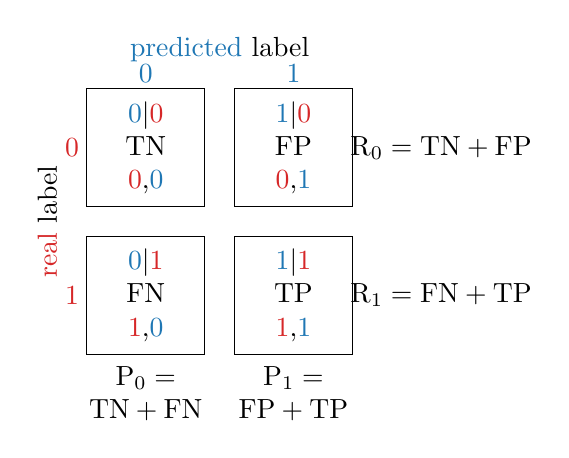
\begin{tikzpicture}[scale=1.25]
\tikzstyle{mtxi}=[draw, shape=rectangle,minimum size=1.5cm]
\tikzstyle{mtxo}=[draw=none, shape=rectangle,minimum size=0.5cm]
\node[mtxi, align=center](tn) at (-0.75,+0.75){$\textcolor{C0}{0} | \textcolor{C3}{0}$\\TN\\\textcolor{C3}{0},\textcolor{C0}{0}};
\node[mtxi, align=center](fp) at (+0.75,+0.75){$\textcolor{C0}{1} | \textcolor{C3}{0}$\\FP\\\textcolor{C3}{0},\textcolor{C0}{1}};
\node[mtxi, align=center](fn) at (-0.75,-0.75){$\textcolor{C0}{0} | \textcolor{C3}{1}$\\FN\\\textcolor{C3}{1},\textcolor{C0}{0}};
\node[mtxi, align=center](tp) at (+0.75,-0.75){$\textcolor{C0}{1} | \textcolor{C3}{1}$\\TP\\\textcolor{C3}{1},\textcolor{C0}{1}};
%
\node[mtxo, align=center](realtrue) at (-1.5,+0.75){$\textcolor{C3}{0}$};
\node[mtxo, align=center](realfalse) at (-1.5,-0.75){$\textcolor{C3}{1}$};
\node[mtxo, align=center](predtrue) at (-0.75,+1.5){$\textcolor{C0}{0}$};
\node[mtxo, align=center](predfalse) at (+0.75,1.5){$\textcolor{C0}{1}$};
%
\node[mtxo, align=center, rotate=90](reallbl) at (-1.75,0){\textcolor{C3}{real} label};
\node[mtxo, align=center](predlbl) at (0,1.75){\textcolor{C0}{predicted} label};
%
\node[mtxo, align=left](realfalse) at (2.25,+0.75){$\text{R}_0 = \text{TN}+\text{FP}$};
\node[mtxo, align=left](realtrue) at (2.25,-0.75){$\text{R}_1 = \text{FN}+\text{TP}$};
%
\node[mtxo, align=center](predfalse) at (-0.75,-1.75){$\text{P}_0 =$\\$\text{TN}+\text{FN}$};
\node[mtxo, align=center](predtrue) at (+0.75,-1.75){$\text{P}_1 =$\\$\text{FP}+\text{TP}$};
%
\end{tikzpicture}
\end{center}
%
\begin{align*}
&\text{ACC}=\frac{\text{TN}+\text{TP}}{\text{R}_0+\text{R}_1}
\qquad
\text{TNR}=\frac{\text{TN}}{\text{R}_0}
\qquad
\text{TPR}=\frac{\text{TP}}{\text{R}_1}
\\
&\text{ACC}=\frac{\text{TN}+\text{TP}}{\text{P}_0+\text{P}_1}
\qquad
\text{NPV}=\frac{\text{TN}}{\text{P}_0}
\qquad
\text{PPV}=\frac{\text{TP}}{\text{P}_1}
\end{align*}
%

\end{frame}



\begin{frame}[t]{Binary Classification Metrics}
%
$\cdot$ TNR = specificity / selectivity, NPV = ?, TPR = sensitivity / recall, PPV = precision

$\cdot$ metric based on TNR and TPR

$\cdot$ metric based on TNR and NPV and/or TPR and PPV

$\cdot$ TPR vs. PPV extrem cases
\begin{align*}
&\text{TPR}=\frac{TP}{R_1}=\frac{TP}{TP+FN}
&\text{PPV}=\frac{TP}{P_1}=\frac{TP}{TP+FP}\\
&\text{TPR}\approx 0: FN \gg TP,\,\,\, TP \approx 0
&\text{PPV}\approx 0: FP \gg TP,\,\,\, TP \approx 0\\
&\text{TPR}\approx 1: TP \gg FN,\,\,\, FN \approx 0
&\text{PPV}\approx 1: TP \gg FP,\,\,\, FP \approx 0\\
\end{align*}
%
$\cdot$ $\text{TPR}\approx 1$ and $\text{PPV}\approx 0$: few FN but many FP (e.g. overestimation of infections)

$\cdot$ $\text{TPR}\approx 0$ and $\text{PPV}\approx 1$: few FP but many FN (e.g. we think we are safe, but are not)

$\cdot$ a potentially meaningful(?!) combination
$$
\left(\frac{\frac{1}{\text{TPR}} + \frac{1}{\text{PPV}}}{2}\right)^{-1}
=
2 \cdot \frac{\text{TPR}\cdot\text{PPV}}{\text{TPR}+\text{PPV}}
=
2 \cdot \frac{\text{recall}\cdot\text{precision}}{\text{recall}+\text{precision}}
=F_1\,\,\,\text{score}
$$

\end{frame}
















% \section{Ex04: Audio Example, Linear Regression, SVD}
% \begin{frame}{Ex04: SVD Factorization of Multitrack Audio}
% Objectives: understanding the essence of SVD vs. utilizing SVD on real data
% %we can listen to audio or view images, so we should bring memorizable examples that feature these senses
%
% \begin{itemize}
% \item given a $M \times N$ matrix $\bm{X}$ with full column rank $r=N$ containing $M$ audio samples on $N$ channels, this might be a studio recording of a song, e.g. 1st channel is bassdrum, 2nd is bass guitar, $N$-th channel is a synth line
% \item perform an economy size SVD on this multitrack audio data (a normal SVD would need way too much RAM to store left nullspace in $\bm{U}$)
% $$\bm{X} = \bm{U} \bm{S} \bm{V}^\mathrm{H}$$
% \item we can listen to and plot the weighted left singular vectors that span the column space
% $$\mathbf{H}_{M \times r} =  \mathbf{U}_{M \times r} \mathbf{S}_{r \times r}$$
% \item we could analyze polarity / level of the mixing weights $\mathbf{V}^\mathrm{H} \mathbf{g}$ of the mixdown
% $$\mathbf{y} = \mathbf{X}\mathbf{g} = \mathbf{H} \cdot \mathbf{V}^\mathrm{H} \mathbf{g}$$
% \item we could listen to the mixdown using the best rank $q<=r$ approximation
% $$\mathbf{y} =\bm{U} \bm{S}_q \bm{V}^\mathrm{H}\mathbf{g}$$
% \end{itemize}
%
% \end{frame}
%
% \section{Ex05: Audio Example}
% \begin{frame}{Ex05: Audio Example}
% Objectives
% %\begin{itemize}
% %\end{itemize}
% \end{frame}
%
%
%
% \section{Section xxx: TBD}
%
% \begin{frame}{Audio Toy Example for Music Genre Classification}
% TBD...
% \end{frame}


% \section{Ex0x: Topic}
% \begin{frame}{Ex0x: Topic}
% Objectives
% \begin{itemize}
% \item
% \end{itemize}
% \end{frame}



%\appendix


%
%
%
















% \section{Appendix}
% \begin{frame}{}
%   $$\im^2=-1, f(x)=x^2$$
%   \begin{figure}
%   \captionsetup{width=.75\linewidth}
%   %\includegraphics[width=\tw\textwidth]{}
%   \caption{.}
%   \label{fig:}
%   \end{figure}
% \end{frame}





\section{Copyright}
\begin{frame}{Copyright}
\begin{itemize}
\item these slides are provided as \href{https://en.wikipedia.org/wiki/Open_educational_resources}{Open Educational Resources} hosted at \href{https://github.com/spatialaudio/data-driven-audio-signal-processing-exercise}{github URL}
\item feel free to use them for your own purposes
\item the text is licensed under \href{https://creativecommons.org/licenses/by/4.0/}{Creative Commons Attribution 4.0}
\item the code snippets of the IPython examples are licensed under the \href{https://opensource.org/licenses/MIT}{MIT license}
\item please attribute the work as follows: Frank Schultz, Data Driven Audio Signal Processing - A Tutorial Featuring Computational Examples, University of Rostock,  ideally with relevant file(s), \href{https://github.com/spatialaudio/data-driven-audio-signal-processing-exercise}{https://github.com/spatialaudio/data-driven-audio-signal-processing-exercise}, commit number and/or version tag, year.
\end{itemize}

\end{frame}
%
\end{document}
